\documentclass[krantz2]{krantz}\usepackage{knitr}%,ChapterTOCs

%\usepackage[utf8]{inputenc}
\usepackage{color}

\usepackage{polyglossia}
\setdefaultlanguage[variant = british, ordinalmonthday = false]{english}

%\usepackage{gitinfo2} % remember to setup Git hooks

\usepackage{hologo}

\usepackage{csquotes}

\usepackage{graphicx}
\DeclareGraphicsExtensions{.jpg,.pdf,.png}

\usepackage{animate}

%\usepackage{microtype}
\usepackage[style=authoryear-comp,giveninits,sortcites,maxcitenames=2,%
    mincitenames=1,maxbibnames=10,minbibnames=10,backref,uniquename=mininit,%
    uniquelist=minyear,sortgiveninits=true,backend=biber]{biblatex}%,refsection=chapter

\newcommand{\href}[2]{\emph{#2} (\url{#1})}

%\usepackage[unicode,hyperindex,bookmarks,pdfview=FitB,%backref,
%            pdftitle={Learn R ...as you learnt your mother tongue},%
%            pdfkeywords={R, statistics, data analysis, plotting},%
%            pdfsubject={R},%
%            pdfauthor={Pedro J. Aphalo}%
%            ]{hyperref}

%\hypersetup{colorlinks,breaklinks,
%             urlcolor=blue,
%             linkcolor=blue,
%             citecolor=blue,
%             filecolor=blue,
%             menucolor=blue}

\usepackage{framed}

\usepackage{abbrev}
\usepackage{usingr}

\usepackage{imakeidx}

% this is to reduce spacing above and below verbatim, which is used by knitr
% to show returned values
\usepackage{etoolbox}
\makeatletter
\preto{\@verbatim}{\topsep=-5pt \partopsep=-4pt \itemsep=-2pt}
\makeatother

%%% Adjust graphic design

% New float "example" and corresponding "list of examples"
%\DeclareNewTOC[type=example,types=examples,float,counterwithin=chapter]{loe}
%\DeclareNewTOC[name=Box,listname=List of Text Boxes, type=example,types=examples,float,counterwithin=chapter,%
%]{lotxb}

% changing the style of float captions
%\addtokomafont{caption}{\sffamily\small}
%\setkomafont{captionlabel}{\sffamily\bfseries}
%\setcapindent{0em}

% finetuning tocs
%\makeatletter
%\renewcommand*\l@figure{\@dottedtocline{1}{0em}{2.6em}}
%\renewcommand*\l@table{\@dottedtocline{1}{0em}{2.6em}}
%\renewcommand*\l@example{\@dottedtocline{1}{0em}{2.3em}}
%\renewcommand{\@pnumwidth}{2.66em}
%\makeatother
%
%% add pdf bookmarks to tocs
%\makeatletter
%\BeforeTOCHead{%
%  \cleardoublepage
%    \edef\@tempa{%
%      \noexpand\pdfbookmark[0]{\list@fname}{\@currext}%
%    }\@tempa
%}

\setcounter{topnumber}{3}
\setcounter{bottomnumber}{3}
\setcounter{totalnumber}{4}
\renewcommand{\topfraction}{0.90}
\renewcommand{\bottomfraction}{0.90}
\renewcommand{\textfraction}{0.10}
\renewcommand{\floatpagefraction}{0.70}
\renewcommand{\dbltopfraction}{0.90}
\renewcommand{\dblfloatpagefraction}{0.70}

\addbibresource{rbooks.bib}
\addbibresource{references.bib}

\makeindex
\IfFileExists{upquote.sty}{\usepackage{upquote}}{}
\begin{document}

% customize chapter format:
%\KOMAoption{headings}{twolinechapter}
%\renewcommand*\chapterformat{\thechapter\autodot\hspace{1em}}

% customize dictum format:
%\setkomafont{dictumtext}{\itshape\small}
%\setkomafont{dictumauthor}{\normalfont}
%\renewcommand*\dictumwidth{0.7\linewidth}
%\renewcommand*\dictumauthorformat[1]{--- #1}
%\renewcommand*\dictumrule{}

%\extratitle{\vspace*{2\baselineskip}%
%             {\Huge\textsf{\textbf{Learn R}\\ \textsl{\huge\ldots as you learnt your mother tongue}}}}

\title{\Huge{\fontseries{ub}\sffamily Learn R\\{\Large\ldots as you learnt your mother tongue}}}

%\subtitle{Git hash: \gitAbbrevHash; Git date: \gitAuthorIsoDate}

\author{Pedro J. Aphalo}

\date{Helsinki, \today}

%\publishers{Draft, 95\% done\\Available through \href{https://leanpub.com/learnr}{Leanpub}}

%\uppertitleback{\copyright\ 2001--2017 by Pedro J. Aphalo\\
%Licensed under one of the \href{http://creativecommons.org/licenses/}{Creative Commons licenses} as indicated, or when not explicitly indicated, under the \href{http://creativecommons.org/licenses/by-sa/4.0/}{CC BY-SA 4.0 license}.}
%
%\lowertitleback{Typeset with \href{http://www.latex-project.org/}{\hologo{XeLaTeX}}\ in Lucida Bright and \textsf{Lucida Sans} using the KOMA-Script book class.\\
%The manuscript was written using \href{http://www.r-project.org/}{R} with package knitr. The manuscript was edited in \href{http://www.winedt.com/}{WinEdt} and \href{http://www.rstudio.com/}{RStudio}.
%The source files for the whole book are available at \url{https://bitbucket.org/aphalo/using-r}.}

%\frontmatter

% knitr setup















% \thispagestyle{empty}
% \titleLL
% \clearpage

\frontmatter

\maketitle

%\begin{titlingpage}
%  \maketitle
%\titleLL
%\end{titlingpage}

\setcounter{page}{7} %previous pages will be reserved for frontmatter to be added in later.
\tableofcontents
%\chapter*{Foreword}
I am delighted to introduce the first book on Multimedia Data Mining.  When I came to know about this book project undertaken by two of the most active young researchers in the field, I was pleased that this book is coming in early stage of a field that will need it more than most fields do.  In most emerging research fields, a book can play a significant role in bringing some maturity to the field.  Research fields advance through research papers.  In research papers, however, only a limited perspective could be provided about the field, its application potential, and the techniques required and already developed in the field.  A book gives such a chance.  I liked the idea that there will be a book that will try to unify the field by bringing in disparate topics already available in several papers that are not easy to find and understand.  I was supportive of this book project even before I had seen any material on it.  The project was a brilliant and a bold idea by two active researchers.  Now that I have it on my screen, it appears to be even a better idea.  

Multimedia started gaining recognition in 1990s as a field.  Processing, storage, communication, and capture and display technologies had advanced enough that researchers and technologists started building approaches to combine information in multiple types of signals such as audio, images, video, and  text.  Multimedia computing and communication techniques recognize correlated information in multiple sources as well as insufficiency of information in any individual source.    By properly selecting sources to provide complementary information, such systems aspire, much like human perception system, to create a holistic picture of a situation using only partial information from separate sources.

Data mining is a direct outgrowth of progress in data storage and processing speeds.  When it became possible to store large volume of data and run different statistical computations to explore all possible and even unlikely correlations among data, the field of data mining was born.  Data mining allowed people to hypothesize relationships among data entities and explore support for those.  This field has been put to applications in many diverse domains and keeps getting more applications.  In fact many new fields are direct outgrowth of data mining and it is likely to become a powerful computational tool.\vadjust{\vfill\pagebreak}



\chapter*{Preface}

\begin{VF}
``Suppose that you want to teach the `cat' concept to a very young child. Do you explain that a cat is a relatively small, primarily carnivorous mammal with retractible claws, a distinctive sonic output, etc.? I'll bet not. You probably show the kid a lot of different cats, saying `kitty' each time, until it gets the idea. To put it more generally, generalizations are best made by abstraction from experience.''

\VA{R. P. Boas}{Can we make mathematics intelligible?}
\end{VF}

%\dictum[R. P. Boas (1981) Can we make mathematics intelligible?, \emph{American Mathematical Monthly} \textbf{88:} 727-731.]{"Suppose that you want to teach the `cat' concept to a very young child. Do you explain that a cat is a relatively small, primarily carnivorous mammal with retractible claws, a distinctive sonic output, etc.? I'll bet not. You probably show the kid a lot of different cats, saying `kitty' each time, until it gets the idea. To put it more generally, generalizations are best made by abstraction from experience."}


% Such pauses are not a miss use of our time. To learn a natural language we need to interact with other speakers, we need feedback. In the case of R, we can get feedback both from the outcomes from our utterances to the computer, and from other \Rlang users.}
\noindent
This book covers different aspects of the use of the \Rlang language. Chapters \ref{chap:R:introduction} to \ref{chap:R:functions} describe the \Rlang language itself. Later chapters describe extensions to the \Rlang language available through contributed \emph{packages}, the \emph{grammar of data} and the \emph{grammar of graphics}. In this book, explanations are concise but contain pointers to additional sources of information, so as to encourage the development of a routine of independent exploration. This is not an arbitrary decision, this is the normal \emph{modus operandi} of most of us who use \Rlang regularly for a variety of different problems. Some have called approaches like the one used here, ``learning the hard way'', but I would call it ``learning to be independent''.

I do not discuss in this book statistics or data analysis methods, I describe \Rlang as a language for data manipulation and display. The idea is for you to learn the \Rlang language in a way comparable to how children learn a language: they work-out what the rules are, simply by listening to people speak and trying to utter what they want to tell their parents. Of course, small children receive some guidance, but are not taught a prescriptive set of rules like when learning a second language at school. Instead of listening, you will read code and instead of speaking you will try to execute \Rlang  code statements on a computer---i.e. you will try your hand at using \Rlang to tell a computer what you want it to compute. I do provide explanations and guidance, but the idea of this book is for you to use the numerous examples to find-out by yourself the overall patterns and coding philosophy behind the \Rlang language. Instead of parents being the sound board for your first utterances in \Rlang, the computer will play this role. You will \emph{play} by modifying the examples, see how the computer responds, does \Rlang understand you or not? Using actively a language is the most efficient way of learning it. By using it, I mean actually reading, writing and running scripts or programs (copying and pasting, or typing ready-made examples from books or the internet does not qualify as using a language).

What is a language? A language is a system of communication. \Rlang as a language allows us to communicate with other members of the \Rlang community, and with computers. As most languages in active use, \Rlang evolves. New ``words'' and new ``constructs'' are incorporated into the language, and some earlier frequently used ones are relegated to the fringes of the corpus. I describe current usage and ``modisms'' of the \Rlang language in a way accessible to a readership unfamiliar with computer science but with some background in data analysis as used in Biology, Engineering, or Humanities.

When teaching I tend to lean towards challenging students rather than telling an over-simplified story. There are two reasons for this. First, I prefer as a student, and I learn best myself if the going is not too easy. Second, if I would hide the tricky bits of the \Rlang language, it would make readers' life much more difficult later on. You, will not remember all the details, nobody could. However, you most likely will remember in which situations you need to be careful or should check the details. So, I will expose you not only the usual cases, but also to several exceptions and counterintuitive features of the language. Reading this book will be about exploring a new world, this book aims to be a travel guide, but neither a traveler's account, nor a cookbook of \Rlang recipes.

Keep in mind that it is impossible to remember everything about \Rlang! The \Rlang language in a broad sense is vast because its capabilities can be expanded with independently developed packages. Learning to use \Rlang consists in learning the basics plus developing the skill of finding your way in \Rlang and its documentation.  In 2017 the number packages available in the Comprehensive \Rlang Archive Network (CRAN) broke the 10\,000 barrier. CRAN is the most important, but not only, public repository for \Rlang packages. How good a command of the \Rlang language and packages a user needs depends on the type activities to be carried out. This book attempts to train you in the use of the \Rlang language itself and of popular \Rlang language extensions for data manipulation and graphical display. Given the availability of numerous books on statistical analysis with \Rlang, in the present book I will cover only the bare minimum of this subject. The same is true for package development in \Rlang. This book seats in-between, aiming at teaching programming in-the-small: the use of \Rlang to automate the drudgery of data manipulation from raw data, through data exploration to the production of publication quality illustrations.

As with all ``rich'' languages there are many different ways of doing things in \Rlang, and there is in almost all cases no one-size-fits-all solution to a problem. There is always a compromise involved, usually between time spent by the user and processing time required in the computer. Many of the packages that are most popular nowadays did not exist when I started using \Rlang, and many of these packages make new approaches available. One could write many different \Rlang books with a given aim using substantially different ways of achieving the same results. In this book, I limit myself to packages that are currently popular and/or that I consider elegantly designed. I have in particular tried to limit myself to packages with similar design philosophies, especially in relation to their interfaces. What is elegant design, and in particular what is a friendly user interface depends strongly on each user's preferences and previous experience. Consequently, the contents of the book are strongly biased by my own preferences. I have tried to write examples in ways that execute fast without compromising readability. I encourage readers to take this book as a starting point for exploring the very many packages, styles and approaches which I have not described.

I will appreciate suggestions for further examples, notification of errors and unclear sections. Many of the examples here have been collected from diverse sources over many years and because of this not all sources are acknowledged. If you recognize any example as yours or someone else's please let me know so that I can add a proper acknowledgement. I warmly thank the students that over the years have asked the questions and posed the problems that have helped me write this text and correct the mistakes and voids of previous versions. I have also received help on on-line forums and in person from numerous people, learnt from archived e-mail list messages, blog posts, books, articles, tutorials, webinars, and by struggling to solve some new problems on my own. In many ways this text owes much more to people who are not authors than to myself. However, as I am the one who has written this version and decided what to include and exclude, as author, I take full responsibility for any errors and inaccuracies.

I have been using \Rlang since around 1998 or 1999, but I am still constantly learning new things about \Rlang itself and \Rlang packages. With time it has replaced in my work as a researcher and teacher several other pieces of software: \pgrmname{SPSS}, \pgrmname{Systat}, \pgrmname{Origin}, \pgrmname{Excel}, and it has become a central piece of the tool set I use for producing lecture slides, notes, books and even web pages. This is to say that it is the most useful piece of software and programming language I have ever learnt to use. Of course, in time it will be replaced by something better, but at the moment it is a key language to learn for anybody with a need to analyse and display data.

Why the title ``\emph{Learn R \ldots as you learnt your mother tongue}''? On one hand, because this book is based on exploration and practice. On the other hand, because you will be exposed to current usage and not spared the quirks of the language. When we use our mother tongue in everyday life we do not think about grammar rules or sentence structure, except for the trickier or unfamiliar situations. My aim is for this book to help you grow to use \Rlang in this same way.

\begin{framed}
\noindent\large%
\textbf{I encourage you to approach R, like a child approaches his or hers mother tongue when learning to speak:} Do not struggle, just play! If going gets difficult and frustrating, take a break! If you get a new insight, take a break to enjoy the victory!
\end{framed}

\newpage

\begin{framed}
\noindent
\textbf{Icons used to mark different content.} Throughout the book text boxes marked with icons present different types of information. First of all, we have \emph{playground} boxes indicated with \playicon\ which contain open-ended exercises---ideas and pieces of \Rlang code to play with at the \Rlang console. A few of these will require more time to grasp, and are indicated with \advplayicon. Boxes providing general information, usually not directly related to \Rlang as a language, are indicated with \infoicon. Some boxes highlighted with \ilAttention\ give important bits of information that must be remembered when using \Rlang---i.e.\ explain some unusual feature of the language. Finally, some boxes indicated by \ilAdvanced\ give in depth explanations, that may require you to spend time thinking, which en general can be skipped on first reading, but to which you should return at a later, and peaceful, time with a cup of coffee or tea.
\end{framed}
\newpage

%\newpage
%\begin{infobox}
%\noindent
%\textbf{Status as of 2016-11-23.} I have updated the manuscript to track package updates since the previous version uploaded six months ago, and added several examples of the new functionality added to packages \ggpmisc, \ggrepel, and \ggplot. I have written new sections on packages \viridis, \pkgname{gganimate}, \pkgname{ggstance}, \pkgname{ggbiplot}, \pkgname{ggforce}, \pkgname{ggtern} and \pkgname{ggalt}. Some of these sections are to be expanded, and additional sections are planned for other recently released packages.
%
%With respect to the chapter \textit{Storing and manipulating data with R} I have put it on hold, except for the introduction, until I can see a soon to be published book covering the same subject. Hadley Wickham has named the set of tools developed by him and his collaborators as \textit{tidyverse} to be described in the book titled \textit{R for Data Science} by Grolemund and Wickham (O'Reilly).
%
%An important update to \ggplot was released last week, and it includes changes to the behavior of some existing functions, specially faceting has become extensible through other packages. Several of the new facilities are described in the updated text and code included in this book and this pdf has been generated with up-to-date version of \ggplot and packages as available today from CRAN, except for \pkgname{ggtern} which was downloaded from Bitbucket minutes ago.
%
%The present update adds about 100 pages to the previous versions. I expect to upload a new update to this manuscript in one or two months time.
%
%\textbf{Status as of 2017-01-17.} Added ``playground'' exercises to the chapter describing \ggplot, and converted some of the examples earlier part of the main text into these playground items. Added icons to help readers quickly distinguish playground sections (\textcolor{blue}{\noticestd{"0055}}), information sections (\textcolor{blue}{\modpicts{"003D}}), warnings about things one needs to be specially aware of (\colorbox{yellow}{\typicons{"E136}}) and boxes with more advanced content that may require longer time/more effort to grasp (\typicons{"E04E}). Added to the sections \code{scales} and examples in the \ggplot chapter details about the use of colors in \Rlang and \ggplot2. Removed some redundant examples, and updated the section on \code{plotmath}. Added terms to the alphabetical index. Increased line-spacing to avoid uneven spacing with inline code bits.
%
%\textbf{Status as of 2017-02-09.} Wrote section on ggplot2 themes, and on using system- and Google fonts in ggpplots with the help of package \pkgname{showtext}. Expanded section on \ggplot's \code{annotation}, and revised some sections in the ``R scripts and Programming'' chapter. Started writing the data chapter. Wrote draft on writing and reading text files. Several other smaller edits to text and a few new examples.
%
%\textbf{Status as of 2017-02-14.} Wrote sections on reading and writing MS-Excel files, files from statistical programs such as SPSS, SyStat, etc., and NetCDF files. Also wrote sections on using URLs to directly read data, and on reading HTML and XML files directly, as well on using JSON to retrieve measured/logged data from IoT (internet of things) and similar intelligent physical sensors, micro-controller boards and sensor hubs with network access.
%
%\textbf{Status as of 2017-03-25.} Revised and expanded the chapter on plotting maps, adding a section on the manipulation and plotting of image data. Revised and expanded the chapter on extensions to \pkgname{ggplot2}, so that there are no longer empty sections. Wrote short chapter ``If and when \Rlang needs help''. Revised and expanded the ``Introduction'' chapter. Added index entries, and additional citations to literature.
%
%\textbf{Status as of 2017-04-04.} Revised and expanded the chapter on using \Rpgrm as a calculator. Revised and expanded the ``Scripts'' chapter. Minor edits to ``Functions'' chapter. Continued writing chapter on data, writing a section on \Rlang native apply functions and added preliminary text for a pipes and tees section. Write intro to `tidyverse' and grammar of data manipulation. Added index entries, and a few additional citations to the literature. Spell checking.
%
%\textbf{Status as of 2017-04-08.} Completed writing first draft of chapter on data, writing all the previously missing sections on the ``grammar of data manipulation''. Wrote two extended examples in the same chapter. Add table listing several extensions to \pkgname{ggplot2} not described in the book.
%
%\textbf{Status as of 2017-04-13.} Revised all chapters correcting some spelling mistakes, adding some explanatory text and indexing all functions and operators used. Thoroughly revised the Introduction chapter and the Preface. Expanded section on bar plots (now bar and column plots). Revised section on tile plots. Expanded section on factors in chapter 2, adding examples of reordering of factor labels, and making clearer the difference between the labels of the levels and the levels themselves.
%
%\textbf{Status as of 2017-04-29.} Tested with R 3.4.0. Package \pkgname{gganimate} needs to be installed from Github as the updated version is not yet in CRAN. Function \code{gg\_animate()} has been renamed \code{gganimate().}
%
%\textbf{Status as of 2017-05-14.} Submitted package \pkgname{learnrbook} to CRAN. Revised code in the book
%to use this new package. Small fixes after more testing. Added examples of plotting and labeling based on fits with \code{method = "nls"}, including use of the new \code{ggpmisc::stat\_fit\_tidy()}.
%
%\textbf{Status as of 2017-06-11.} Added sections on R-code bench marking and profiling for performance optimization. Added also an example of explicit compilation of a function defined in the R language. Added section on functions \code{assign()}, \code{get()} and \code{mget()}.
%
%\textbf{Status as of 2017-08-12.} Various edits to all chapters. Expanded section on \pkgname{ggpmisc} to include the new functionality added in version 0.2.15.9002: \code{geom\_table} and \code{stat\_fit\_tb}. Added section on package \pkgname{ggbeeswarm}. Added sections on packages \pkgname{magick} and on using \pgrmname{ImageJ} from \Rpgrm. Improved indexing and cross references.
%
%\textbf{Status as of 2017-10-25.} Edited the chapter on using R as a calculator, adding examples on insertion and deletion of members of lists and vectors, and also of use of \code{gl()} and \code{reorder()}. Edited sections on scale limits and added new section on coordinate limits to explain more thoroughly their differences and uses in chapter on plotting with \pkgname{ggplot2}. Added a section on package \pkgname{ggsignif} to the chapter on extensions to \pkgname{ggplot2}. Expanded section on \pkgname{ggpmisc} in the same chapter describing new functionality added in version 0.2.16.
%\pkgname{ggplo2} $>=$ 2.2.1.9000 is required by the current development version of \pkgname{ggpmisc}.
%
%\textbf{Status as of 2017-10-30.}  Add section on using pipes with \code{ggplot()} and layers.
%\end{infobox} 
\listoffigures
\listoftables
%%%\twocolumn
\chapter*{Contributors}

\begin{multicols}{2}
\contributor{Michael Aftosmis}{NASA Ames Research Center}{Moffett Field, California}

\contributor{Pratul K. Agarwal}{Oak Ridge National Laboratory}{Oak Ridge, Tennessee}

\contributor{Sadaf R. Alam}{Oak Ridge National Laboratory}{Oak Ridge, Tennessee}

\contributor{Gabrielle Allen}{Louisiana State University}{Baton Rouge, Louisiana}

\contributor{Martin Sandve Aln{\ae}s}{Simula Research Laboratory and University of Oslo, Norway}{Norway}

\contributor{Steven F. Ashby} {Lawrence Livermore National Laboratory}{Livermore, California}

\contributor{David A. Bader} {Georgia Institute of Technology}{Atlanta, Georgia}

\contributor{Benjamin Bergen} {Los Alamos National Laboratory}{Los Alamos, New Mexico}

\contributor{Jonathan W. Berry} {Sandia National Laboratories}{Albuquerque, New Mexico}

\contributor{Martin Berzins}{University of Utah}{Salt Lake City, Utah}

\contributor{Abhinav Bhatele}{University of Illinois}{Urbana-Champaign, Illinois}

\contributor{Christian Bischof} {RWTH Aachen University}{Germany}

\contributor{Rupak Biswas} {NASA Ames Research Center}{Moffett Field, California}\vspace*{5pt}

\contributor{Eric Bohm} {University of Illinois}{Urbana-Champaign, Illinois}\vspace*{5pt}

\contributor{James Bordner} {University of California, San Diego}{San Diego, California}\vspace*{5pt}

\contributor{George Bosilca} {University of Tennessee}{Knoxville, Tennessee}\vspace*{5pt}

\contributor{Greg L. Bryan} {Columbia University}{New York, New York}\vspace*{5pt}

\contributor{Marian Bubak} {AGH University of Science and Technology}{
Krak{\'o}w, Poland}\vspace*{5pt}

\contributor{Andrew Canning}{Lawrence Berkeley National
Laboratory}{Berkeley, California}

\contributor{Jonathan Carter} {Lawrence Berkeley National
Laboratory}{Berkeley, California}

\contributor{Zizhong Chen} {Jacksonville State University}{Jacksonville,
Alabama}

\contributor{Joseph R. Crobak} {Rutgers, The State University of New
Jersey}{Piscataway, New Jersey}

\contributor{Roxana E. Diaconescu} {Yahoo! Inc.}{Burbank, California}

\contributor{Peter Diener}
{Louisiana State University}{Baton Rouge, Louisiana}

\contributor{Jack J. Dongarra} {University of Tennessee, Knoxville, 
Oak Ridge National Laboratory, and}{University of Manchester}

\contributor{John B. Drake} {Oak Ridge National Laboratory}{Oak Ridge,
Tennessee}

\contributor{Kelvin K. Droegemeier} {University of Oklahoma}{Norman,
Oklahoma}

\contributor{St{\'e}phane Ethier} {Princeton University}{Princeton, New
Jersey}

\contributor{Christoph Freundl}
{Friedrich--Alexander--Universit{\"a}t}{Erlangen, Germany}

\contributor{Karl F{\"u}rlinger} {University of Tennessee}{Knoxville,
Tennessee}

\contributor{Al Geist} {Oak Ridge National Laboratory}{Oak Ridge,
Tennessee}

\contributor{Michael Gerndt} {Technische Universit{\"a}t
M{\"u}nchen}{Munich, Germany}

\contributor{Tom Goodale}
{Louisiana State University}{Baton Rouge, Louisiana}

\contributor{Tobias Gradl}
{Friedrich--Alexander--Universit{\"a}t}{Erlangen, Germany}

\contributor{William D. Gropp} {Argonne National Laboratory}{Argonne,
Illinois}

\contributor{Robert Harkness} {University of California, San
Diego}{San Diego, California}

\contributor{Albert Hartono} {Ohio State University}{Columbus, Ohio}

\contributor{Thomas C. Henderson} {University of Utah}{Salt Lake City,
Utah}

\contributor{Bruce A. Hendrickson} {Sandia National
Laboratories}{Albuquerque, New Mexico}

\contributor{Alfons G. Hoekstra} {University of Amsterdam}{Amsterdam,
The Netherlands}

\contributor{Philip W. Jones} {Los Alamos National Laboratory}{Los
Alamos, New Mexico}

\contributor{Laxmikant Kal{\'e}} {University of
Illinois}{Urbana-Champaign, Illinois}

\contributor{Shoaib Kamil} {Lawrence Berkeley National
Laboratory}{Berkeley, California}

\contributor{Cetin Kiris} {NASA Ames Research Center}{Moffett Field,
California}

\contributor{Uwe K{\"u}ster} {University of Stuttgart}{Stuttgart,
Germany}

\contributor{Julien Langou} {University of Colorado}{Denver, Colorado}

\contributor{Hans Petter Langtangen}
{Simula Research Laboratory and}{University of Oslo, Norway}

\contributor{Michael Lijewski} {Lawrence Berkeley National
Laboratory}{Berkeley, California}

\contributor{Anders Logg}
{Simula Research Laboratory and}{University of Oslo, Norway}

\contributor{Justin Luitjens} {University of Utah}{Salt Lake City, Utah}

\contributor{Kamesh Madduri} {Georgia Institute of Technology}{Atlanta,
Georgia}

\contributor{Kent-Andre Mardal}
{Simula Research Laboratory and}{University of Oslo, Norway}

\contributor{Satoshi Matsuoka} {Tokyo Institute of Technology}{Tokyo,
Japan}

\contributor{John M. May} {Lawrence Livermore National
Laboratory}{Livermore, California}

\contributor{Celso L. Mendes} {University of Illinois}{Urbana-Champaign,
Illinois}

\contributor{Dieter an Mey} {RWTH Aachen University}{Germany}

\contributor{Tetsu Narumi} {Keio University}{Japan}

\contributor{Michael L. Norman} {University of California, San
Diego}{San Diego, California}

\contributor{Boyana Norris} {Argonne National Laboratory}{Argonne,
Illinois}

\contributor{Yousuke Ohno} {Institute of Physical and Chemical Research
(RIKEN)}{Kanagawa, Japan}

\contributor{Leonid Oliker} {Lawrence Berkeley National
Laboratory}{Berkeley, California}

\contributor{Brian O'Shea} {Los Alamos National Laboratory}{Los Alamos,
New Mexico}

\contributor{Christian D. Ott}
{University of Arizona}{Tucson, Arizona}

\contributor{James C. Phillips} {University of
Illinois}{Urbana-Champaign, Illinois}

\contributor{Simon Portegies Zwart} {University of
Amsterdam,}{Amsterdam, The Netherlands}

\contributor{Thomas Radke}
{Albert-Einstein-Institut}{Golm, Germany}

\contributor{Michael Resch} {University of Stuttgart}{Stuttgart,
Germany}

\contributor{Daniel Reynolds} {University of California, San Diego}{San
Diego, California}

\contributor{Ulrich R{\"u}de}
{Friedrich--Alexander--Universit{\"a}t}{Erlangen, Germany}

\contributor{Samuel Sarholz}
{RWTH Aachen University}{Germany}

\contributor{Erik Schnetter}
{Louisiana State University}{Baton Rouge, Louisiana}

\contributor{Klaus Schulten} {University of Illinois}{Urbana-Champaign,
Illinois}

\contributor{Edward Seidel}
{Louisiana State University}{Baton Rouge, Louisiana}

\contributor{John Shalf} {Lawrence Berkeley National
Laboratory}{Berkeley, California}

\contributor{Bo-Wen Shen} {NASA Goddard Space Flight Center}{Greenbelt,
Maryland}

\contributor{Ola Skavhaug}
{Simula Research Laboratory and}{University of Oslo, Norway}

\contributor{Peter M.A. Sloot} {University of Amsterdam}{Amsterdam, The
Netherlands}

\contributor{Erich Strohmaier} {Lawrence Berkeley National
Laboratory}{Berkeley, California}

\contributor{Makoto Taiji} {Institute of Physical and Chemical Research
(RIKEN)}{Kanagawa, Japan}

\contributor{Christian Terboven}
{RWTH Aachen University,}{Germany}

\contributor{Mariana Vertenstein} {National Center for Atmospheric
Research}{Boulder, Colorado}

\contributor{Rick Wagner} {University of California, San Diego}{San
Diego, California}

\contributor{Daniel Weber} {University of Oklahoma}{Norman, Oklahoma}

\contributor{James B. White, III} {Oak Ridge National Laboratory}{Oak
Ridge, Tennessee}

\contributor{Terry Wilmarth} {University of Illinois}{Urbana-Champaign,
Illinois}

\end{multicols}
%\chapter*{Symbols}
\begin{symbollist}{000000}
\symbolentry{$\alpha$}{To solve the generator maintenance scheduling, in the  past, several mathematical techniques have  been applied.}
\symbolentry{$\sigma^2$}{These include integer programming, integer linear programming, dynamic programming, branch and bound etc.}
\symbolentry{$\sum$}{Several heuristic search algorithms have also been developed. In recent years expert systems,}
\symbolentry{$abc$}{fuzzy approaches, simulated annealing and genetic algorithms have also been tested.}
\symbolentry{$\theta\sqrt{abc}$}{This paper presents a survey of the literature}
\symbolentry{$\zeta$}{ over the past fifteen years in the generator}
\symbolentry{$\partial$}{maintenance scheduling. The objective is to}
\symbolentry{sdf}{present a clear picture of the available recent literature}
\symbolentry{ewq}{of the problem, the constraints and the other aspects of}
\symbolentry{bvcn}{the generator maintenance schedule.}
\end{symbollist}

\mainmatter




% !Rnw root = using-r.main.Rnw



\chapter{Introduction}\label{chap:R:introduction}

\begin{VF}
The creative adult is the child who has survived.

\VA{Ursula K. le Guin}{}
\end{VF}

%\dictum[Ursula K. le Guin]{The creative adult is the child who has survived.}\vskip2ex

\section{R}

\subsection{What is R?}

Most people think of \Rpgrm as a computer program. \Rpgrm is indeed a computer program---a piece of software---, but it is also a computer language, implemented in the \Rpgrm program. Does this make a difference? Yes, until recently we had only one mainstream implementation of \Rlang, the program \Rpgrm. In the last couple of years another implementation has started to gain popularity, \pgrmname{Microsoft R}, which is directly based on the \Rpgrm from \textit{The R Project for Statistical Computing}. These two very similar implementations are not the only ones available, but others are not in widespread use. In other words, the \Rlang language can be used not only in the \Rpgrm program, and is feasible that other implementations will be developed in the future.

Being \Rpgrm essentially a command line application, it can be used on what nowadays are frugal computing resources, equivalent to a personal computer of a couple of decades ago. \Rpgrm can run even on the Raspberry Pi\index{Raspberry Pi}, a micro-controller board with the processing power of a modest smartphone. At the other end of the spectrum on really powerful servers, \Rpgrm can be used for the analysis of big data sets with millions of observations. How powerful a computer you will need will depend on the size of the data sets you want to analyze, and on how patient you are, and on your ability to write `good' code.

One could think of \Rlang, as a dialect of an earlier language, called \Slang. \Slang evolved into \Splang. \Slang and \Splang are commercial programs, and variations in the language appeared only between versions. \Rlang started as a poor man's home-brewed implementation of \Slang, for use in teaching. Initially \Rpgrm, the program, implemented a subset of the \Slang language. The \Rpgrm program evolved until only relatively few differences between \Slang and \Rlang remained, and these differences are intentional---thought of as significant improvements. As \Rlang overtook \Splang in popularity, some of the new features in \Rlang made their way back into \Splang. \Rpgrm being free and open-source is sometimes called \pgrmname{Gnu S}.

What makes \Rlang different from \pgrmname{SPSS}, \pgrmname{SAS}, etc., is that \Slang was designed as a computer programming language. This may look unimportant for someone not actually needing or willing to write software for data analysis. However, in reality it makes a huge difference because \Rlang is easily extensible. By this we mean that new functionality can be easily added, and shared, and this new functionality is to the user indistinguishable from that built-in into \Rlang. It other words, instead of having to switch between different pieces of software to do different types of analyses or plots, one can usually find an \Rlang package that will provide the tools to do the job within \Rlang. For those routinely doing similar analyses the ability to write a short program, sometimes just a handful of lines of code, will allow automation of routine analyses. For those willing to spend time programming, they have to door open to building the tools they need if these do not already exist.

However, the most import advantage of using a language like \Rlang is that it makes it easy to do data analyses in a way that ensures that they can be exactly repeated. In other words, the biggest advantage of using \Rlang, as a language, is not in communicating with the computer, but in communicating to other people what has been done, in a way that is unambiguous. Of course, other people may want to run the same commands in another computer, but still it means that a translation from a set of instructions to the computer into text readable to humans---say the materials and methods section of a paper---and back is avoided together with the ambiguities usually creeping in.

\subsection{R as a language}
\index{R as a language}
\Rlang is a computer language designed for data analysis and data visualization, however, in contrast to some other scripting languages, it is from the point of view of computer programming a complete language---it is not missing any important feature. In other words no basic operations or data types are lacking.

As mentioned above, \Rlang started as a free and open-source implementation of the \Slang language \autocite{Becker1984,Becker1988}. We will describe the features of the \Rlang language on later chapters. Here I mention, for those with programming experience, that it does have some features that makes it different from other frequently used programming languages. For example, \Rlang does not have the strict type checks of \langname{Pascal} or  \Cpplang. It also has operators that can take vectors and matrices as operands allowing  more concise program statements for such operations than other languages. Writing programs, specially reliable and fast code, requires familiarity with some of these idiosyncracies of the R language. For those using R interactively, or writing short scripts, these idiosyncratic features also make life a lot easier by saving typing.

\begin{explainbox}
Some languages have been standardised, and their grammar has been formally defined. \Rlang, in contrast is not standardized, and there is no formal grammar definition. So, the \Rlang language is defined by the behaviour of the \Rpgrm program.
\end{explainbox}

\subsection{R as a computer program}
\index{R as a computer program}
The \Rpgrm program itself is open-source, the source code is available for anybody to inspect, modify and use. A small fraction of users will directly contribute improvements to the \Rpgrm program itself, but it is possible, and those contributions are important in making \Rpgrm reliable. The executable, the \Rpgrm program we actually use, can be built for different operating systems and computer hardware. The members of the \Rpgrm developing team make an important effort to keep the results obtained from calculations done on all the different builds and computer architectures as consistent as possible. The aim is to ensure that computations return consistent results not only across updates to \Rpgrm but also across different operating systems like \osname{Linux}, \osname{Unix} (including \osname{OS X}), and \osname{MS-Windows}, and computer hardware.

\begin{figure}
  \centering
  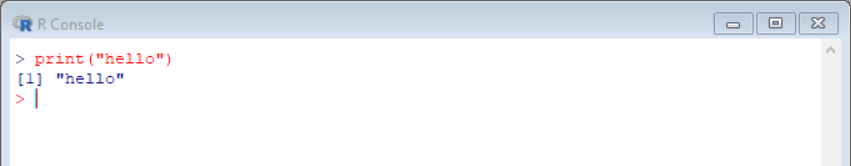
\includegraphics[width=0.85\textwidth]{figures/R-console-r}
  \caption[The R console]{The \Rpgrm console where the user can type textual commands one by one. Here the user has typed \code{print("Hello")} and \textit{entered} it by ending the line of text by pressing the ``enter'' key. The result of running the command is displayed below the command. The character at the head of the input line, a ``$>$'' in this case, is called the command prompt, signalling where a command can be typed in. Commands entered by the user are displayed in red, while results returned by R are displayed in blue.}\label{fig:intro:console}
\end{figure}

The \Rpgrm program does not have a graphical user interface (GUI), or menus from which to start different types of analyses. Instead, the user types the commands at the \Rpgrm console (Figure \ref{fig:intro:console}). The commands can be also saved into a text file, line by line, and such the file, called a `script' can substitute repeated typing of the same sequence of commands. When we work at the console typing in commands one by one, we say that we use R interactively. When we run script we may say that we run a ``batch job''.

The two approaches described above are part of the \Rpgrm program by itself. However, it is common to use a second program as a front-end or middle man ``in-between'' the user and the \Rpgrm program. Such a program allows more flexibility and has multiple features that makes entering commands or writing scripts easier---in other words makes it easier for the user to interact with \Rpgrm. Computations are still done by exactly the same \Rpgrm program. The simplest option is to use a text editor like \pgrmname{Emacs} to edit the scripts and then run the scripts in \Rpgrm from within the editor. With some editors like \pgrmname{Emacs}, rather good integration is possible. However, nowadays there are also Integrated Development Environments (IDEs) available for \Rpgrm. An IDE gives access to both use of the \Rpgrm console in a window, and provides a text editor for writing scripts in a separate window. Of the available IDEs for \Rpgrm, \RStudio is currently the most popular by a wide margin.

\subsubsection{Using R interactively}

A physical terminal (keyboard plus text-only screen) decades ago was how users communicated with computers, and was frequently called \emph{console}\index{console}. Nowadays, a text-only interface to a computer, in most cases a window or a pane within a graphical user interface it is still called a console. In our case, the \Rpgrm console (Figure \ref{fig:intro:console}). This is the native user interface of \Rpgrm.

Typing commands at the \Rpgrm console is useful when one is playing around, rather aimlessly exploring things, or trying to understand how an \Rpgrm function or operator we are not familiar with works. Once we want to keep track of what we are doing, there are better ways of using \Rpgrm, which allow us to keep a record of how an analysis has been carried out. The different ways of using \Rpgrm are not exclusive of each other, so most users will use the \Rpgrm console to test individual commands and plot data during the first stages of exploration. As soon as we decide how we want to plot or analyse the data, it is best to start using scripts. This is not enforced in any way by \Rpgrm, but scripts are what really brings to light the most important advantages of using a programming language for data analysis. In Figure \ref{fig:intro:console} we can see how the \Rpgrm console looks. The text in red has been typed in by the user---except for the prompt \code{$>$}---, and the text in blue is what \Rpgrm has displayed in response. It is essentially a dialogue between user and \Rpgrm. The console can \emph{look} different when displayed within an IDE like \RStudio, but the only difference is in the appearance of the text rather than in the text itself (cf.\ Figures \ref{fig:intro:console} and \ref{fig:intro:console:rstudio}).

\begin{figure}
  \centering
  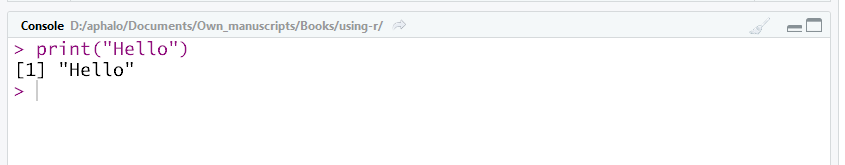
\includegraphics[width=\linewidth]{figures/r-console-rstudio}
  \caption[The R console]{The \Rpgrm console embedded in \RStudio. The same commands have been typed-in as in Figure \ref{fig:intro:console}. Commands entered by the user are displayed in purple, while results returned by \Rpgrm are displayed in black.}\label{fig:intro:console:rstudio}
\end{figure}

The two previous figures showed the result of entering a single command. Figure \ref{fig:intro:console:capture} shows how the console looks after the user has entered several commands, each as a separate line of text.

\begin{figure}
  \centering
  \includegraphics[width=\linewidth]{figures/r-console-capture}
  \caption[The R console]{The \Rpgrm console after several commands have been entered. Commands entered by the user are displayed in red, while results returned by \Rpgrm are displayed in blue.}\label{fig:intro:console:capture}
\end{figure}

The examples in this book require only the console window for user input. Menu-driven programs are not necessarily bad, they are just unsuitable when there is a need to set very many options and choose from many different actions. They are also difficult to maintain when extensibility is desired, and when independently developed modules of very different characteristics need to be integrated. Textual languages also have the advantage, to be dealt in later chapters, that command sequences can be stored in human- and computer readable text files. Such files constitute a record of all the steps used and in most cases makes it trivial to reproduce the same steps at a later time. Scripts are also a very simple and handy way of communicating to others how to do a given data analysis. When working at the command prompt, most results are printed by default, but in within scripts one needs to use the function \Rfunction{print()} explicitly.

\begin{explainbox}
In the console one types commands at the \code{>} prompt. When one ends a line by pressing the return or enter key, if the line can be interpreted as an R command, the result will be printed at the console, followed by a new \code{>} prompt.
If the command is incomplete a \code{+} continuation prompt will be shown, and you will be able to type-in the rest of the command. For example if the whole calculation that you would like to do is $1 + 2 + 3$, if you enter in the console \code{1 + 2 +} in one line, you will get a continuation prompt where you will be able to type \code{3}. However, if you type \code{1 + 2}, the result will be calculated, and printed.
\end{explainbox}

\subsubsection{Using R as a ``batch job''}

To run a script we need first to prepare a script in a text editor. Figure \ref{fig:intro:script} shows the console immediately after running the script file shown in the lower window. As before, red text, the command \code{source("my-script.R")}, was typed by the user, and the blue text in the console is what was displayed by \Rpgrm as a result of this action.

\begin{figure}
  \centering
  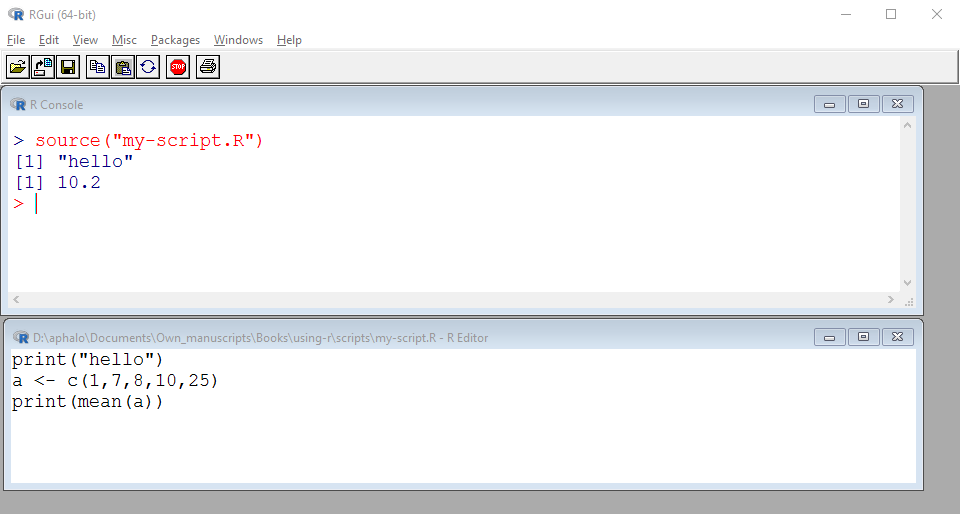
\includegraphics[width=\linewidth]{figures/R-console-script}
  \caption[Script sourced at the R console]{Screen capture of the \Rpgrm console and editor just after running a script. The upper window shows the \Rpgrm console, and the lower window the script file in an editor window. }\label{fig:intro:script}
\end{figure}

A true ``batch job'' is not run at the \Rpgrm console but at the operating system command prompt, or shell. The shell is the console of the operating system---\osname{Linux}, \osname{Unix}, \osname{OS X}, or \osname{MS-Windows}. Figure \ref{fig:intro:shell} shows how running an script at the Windows commands prompt looks. In normal use, a script is run at the operating system prompt to do time-consuming calculations and the output is saved to a file. One may use this approach on a server, say, to leave a large data analysis job running over-night.

\begin{figure}
  \centering
  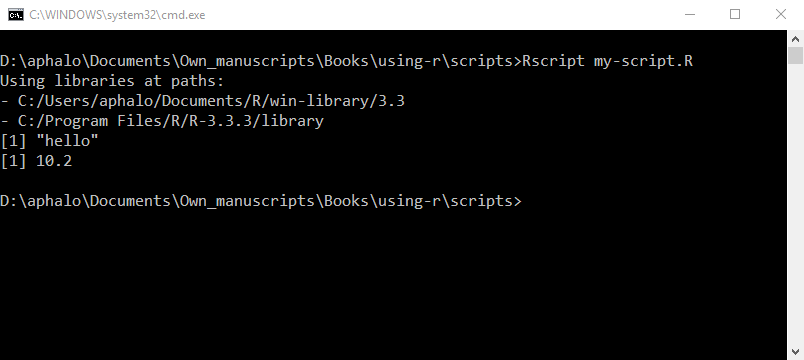
\includegraphics[width=\linewidth]{figures/windows-cmd-script}
  \caption[Script at the Windows cmd promt]{Screen capture of the \osname{MS-Windows} command console just after running the same script. Here we use \code{Rscript} to run the script, the exact syntax will depend on the operating system in use. In this case \Rpgrm prints the results at the operating system console or shell, rather than in its own \Rpgrm console.}\label{fig:intro:shell}
\end{figure}

\subsubsection{Editors and IDEs}

Integrated Development Environments (IDEs) were initially created for computer program development. IDEs provide a centralized user interface from within which the different tools used to create and test a computer program can be used in coordination. Most IDEs include a dedicated editor capable of syntax highlighting, and even report some mistakes, related to the programming language in use while the user types. One could describe such editor as the equivalent as a word processor with spelling and grammar checking, that can alert about spelling and syntax errors for a computer language like \Rlang instead of for a natural language like English. In the case of \RStudio, the main, but not only language supported is \Rlang. The main window of IDEs usually displays more than one pane simultaneously. From within the \RStudio IDE one has access to the \Rpgrm console, a text editor, a file-system browser, and access to several additional tools. Although \RStudio supports very well the development of large scripts and packages, it is also the best possible way of using \Rpgrm at the console as it has the \Rpgrm help system very well integrated. Figure \ref{fig:intro:rstudio} shows the main window displayed by \RStudio after running the same script as shown above at the \Rpgrm console (Figure \ref{fig:intro:script}) and at the operating system command prompt (Figure \ref{fig:intro:shell}). We can see by comparing these three figures how \RStudio is really a layer between the user and an unmodified \Rpgrm executable. The script was sourced by pressing the ``Source'' button at the top of the editor pane. \RStudio in response to this generated the code needed to source the file and ``entered'' it at the console, the same console, where we would type ourselves any \Rpgrm commands.

\begin{figure}
  \centering
  \includegraphics[width=\linewidth]{figures/Rstudio-script}
  \caption[Script in Rstudio]{The \RStudio interface just after running the same script. Here we used the ``Source'' button to run the script. In this case \Rpgrm prints the results to the \Rpgrm console in the lower left pane.}\label{fig:intro:rstudio}
\end{figure}

When a script is run, if an error is triggered, \RStudio automatically finds the location of the error. \RStudio also supports the concept of projects allowing saving of settings per project. Some features are beyond what you need for everyday data analysis and aimed at package development, such as integration of debugging, traceback on errors, profiling and bench marking of code so as to analyse and improve performance. It also integrates support for file version control, which is not only useful for package development, but also for keeping track of the progress or collaboration in the analysis of data.

The version of \RStudio that one uses locally, i.e.\ installed in your own computer, runs with almost identical user interface on most modern operating systems, such as \osname{Linux}, \osname{Unix}, \osname{OS X}, and \osname{MS-Windows}. There is also a server version that runs on \osname{Linux}, and that can be used remotely through a web browser. The user interface is still the same.

\RStudio is under active development, and constantly improved. Visit \url{http://www.rstudio.org/} for an up-to-date description and download and installation instructions. Two books \autocite{vanderLoo2012,Hillebrand2015} describe and teach how to use \RStudio without going in depth into data analysis or statistics, however, as \RStudio is under very active development several recently added important features are not described in these books. You will find tutorials and up-to-date cheat sheets at \url{http://www.rstudio.org/}.

\section{Packages and repositories}
\index{packages!extending R}
The most elegant way of adding new features or capabilities to \Rlang is through packages. This is without doubt the best mechanism when these extensions to \Rlang need to be shared. However, in most situations it is also the best mechanism for managing code that will be reused even by a single person over time. \Rlang packages have strict rules about their contents, file structure, and documentation, which makes it possible among other things for the package documentation to be merged into \Rpgrm's help system when a package is loaded. With a few exceptions, packages can be written so that they will work on any computer where \Rpgrm runs.

Packages can be shared as source or binary package files, sent for example through e-mail. However, for sharing packages widely, best is to submit them to a repository. The largest public repository of \Rpgrm packages is called CRAN\index{CRAN}, an acronym for Comprehensive R Archive Network. Packages available through CRAN are guaranteed to work, in the sense of not failing any tests built into the package and not crashing or aborting prematurely. They are tested daily, as they may depend on other packages whose code will change when updated. In January 2017, the number of packages available through CRAN passed the 10\,000 mark.

Using packages requires in general two steps: 1) installing the package into the \Rpgrm library\index{packages!library}\index{packages!installation} and 2) loading it from the library into the current \Rpgrm session\index{packages!loading}. Installation is needed once and consists in making a local copy of the package. Loading needs to be done at least once in each \Rpgrm session, and before any command defined in the package can be used. Loading a package also loads the corresponding help pages.

Packages are installed into the library using function \Rfunction{install.packages()} and are loaded from the library with function \Rfunction{library()}.

\begin{playground}
  Use \code{help} to look up the help pages for \code{install.packages} and \code{library}, and explain what the code in the next chunk does.
\begin{knitrout}\footnotesize
\definecolor{shadecolor}{rgb}{0.969, 0.969, 0.969}\color{fgcolor}\begin{kframe}
\begin{alltt}
\hlkwd{install.packages}\hlstd{(learnrbook)}
\hlkwd{library}\hlstd{(learnrbook)}
\hlkwd{help}\hlstd{(learnrbook)}
\end{alltt}
\end{kframe}
\end{knitrout}
\end{playground}

When using an IDE like \RStudio, although these commands can be typed into the \Rpgrm console, it is usually easier to manage installation and update of packages through the IDE's interface, which in turn generates the needed \Rlang code and runs it in the console.

Loading of packages seems to me easier directly at the console or as part of a script. Of course, this is my own preference that may differ from yours.

\section{Reproducible data analysis}
\index{reproducible data analysis|(}
Reproducible data analysis is much more than a fashionable buzzword. Under any situation where accountability is important, from scientific research to decision making in commercial enterprises, industrial quality control and safety and impact assessments, being able to reproduce a data analysis reaching the same conclusions from the same data is crucial. Most approaches to reproducible data analysis are based on automating report generation and including as part of the report all the computer commands used to generate the results presented.

A fundamental requirement for reproducibility, is a reliable record of what commands have been run on which data. Such a record is specially difficult to keep when issuing commands through menus and dialogue boxes in a graphical user interface or interactively at a console. Even working interactively at the \Rpgrm console using copy and paste to include commands and results in a report is error prone, and laborious.

A further requirement is to be able to match the output of the \Rlang commands to the input. If the script saves the output to separate files, then the user will need to take care that the script saved or shared as record of the data analysis was the one actually used for obtaining the reported results and conclusions. This is another error prone stage in the report of a data analysis. To solve this problem an approach was developed, inspired in what is called \emph{literate programming} \autocite{Knuth1984a}. The idea is that running the script will produce a document that includes the script, the results of running the scripts and any explanatory text needed to understand and interpret the analysis.

Although a system capable of producing such reports with \Rlang, called \pkgname{Sweave} \autocite{Leisch2002}, has been available for a couple decades, it was rather limited and not supported by an IDE, making its use rather tedious. A more recently developed system called \pkgname{knitr} \autocite{Xie2013} together with its integration into \RStudio has made the use of this type of reports very easy. The most recent development are \emph{notebooks} produced within \RStudio. This new feature, can produce the readable report of running the script as an HTML file, including the code used interspersed with the results within the viewable file as in earlier approaches. However, this newer approach goes even further: the actual source script used to generate the report is embedded in the HTML file of the report and can be extracted and run very easily. This means that anyone who gets access to the output of the analysis in human readable form also gets access to the code used to generate the report, in computer executable format.

Because of these recent developments, \Rlang is an ideal language to use when the goal of reproducibility is important. During recent years the problem of the lack of reproducibility in scientific research has been broadly discussed and analysed \autocite{Gandrud2015}. One on the problems faced when attempting to reproduce experimental work, is reproducing the data analysis. \Rlang together with these modern tools can help in avoiding this source of lack of reproducibility.

How powerful are these tools? and how flexible? They are powerful and flexible enough to write whole books, such as this very book you are now reading, produced with \Rpgrm, \pkgname{knitr} and \LaTeX\index{Latex@\LaTeX}. All pages in the book are generated directly, all figures are generated by \Rpgrm and included automatically, except for the figures in this chapter that have been manually captured from the computer screen. Why am I using this approach? First because I want to make sure that every bit of code as you will see printed, runs without error. In addition I want to make sure that the output that you will see below every line or chunk of \Rlang language code is exactly what \Rpgrm returns. Furthermore, it saves a lot of work for me as author, as I can just update \Rpgrm and all the packages used to their latest version, and build the book again, to keep it up to date and free of errors.

Although the use of these tools is important, they are outside the scope of this book and well described in other book \autocite{Gandrud2015,Xie2013}. Still when writing code, using a consistent style for formatting and indentation, carefully choosing variable names, and adding textual explanations in comments when needed, helps very much with readability for humans. I have tried to be as consistent as possible throughout the whole book in this respect, with only small personal deviations from the usual style.
\index{reproducible data analysis|)}

\section{Finding additional information}

When searching for answers, asking for advice or reading books you will be confronted with different ways of approaching the same tasks. Do not allow this to overwhelm you, in most cases it will not matter as many computations can be done in \Rpgrm, as in any language, in several different ways, still obtaining the same result. The different approaches may differ mainly in two aspects: 1) how readable to humans are the instructions given to the computer as part of a script or program, and 2) how fast the code runs. Unless performance is an important bottleneck in your work, just concentrate on writing code that is easy to understand to you and to others, and consequently easy to check and reuse. Of course do always check any code you write for mistakes, preferably using actual numerical test cases for any complex calculation or even relatively simple scripts. Testing and validation are extremely important steps in data analysis, so get into this habit while reading this book. Testing how every function works as I will challenge you to do in this book, is at the core of any robust data analysis or computing programming. When developing \Rlang packages, including a good coverage of test cases as part of the package itself simplifies code maintenance enormously, helps in maintaining consistency of behaviour across versions, and reveals in good time problems triggered by updates to \Rpgrm or packages depended upon.

\subsection{R's built-in help}

To\index{R!help} access help pages through the command prompt we use function \Rfunction{help()} or a question mark. Every object exported by an \Rlang package (functions, methods, classes, data) is documented. Sometimes a single help page documents several \Rlang objects. Usually at the end of the help pages, some examples are given, which tend to help very much in learning how to use the functions described. For example one can search for a help page at the \Rpgrm console.

\begin{knitrout}\footnotesize
\definecolor{shadecolor}{rgb}{0.969, 0.969, 0.969}\color{fgcolor}\begin{kframe}
\begin{alltt}
\hlkwd{help}\hlstd{(}\hlstr{"sum"}\hlstd{)}
\hlopt{?}\hlstd{sum}
\end{alltt}
\end{kframe}
\end{knitrout}

\begin{playground}
Look at help for some other functions like \code{mean()}, \code{var()}, \code{plot()} and, why not, \Rfunction{help()} itself!
\begin{knitrout}\footnotesize
\definecolor{shadecolor}{rgb}{0.969, 0.969, 0.969}\color{fgcolor}\begin{kframe}
\begin{alltt}
\hlkwd{help}\hlstd{(help)}
\end{alltt}
\end{kframe}
\end{knitrout}
\end{playground}

When using \RStudio there are easier ways of navigating to a help page than using function \Rfunction{help()}, for example with the cursor on the name of a function in the editor or console, pressing the F1 key, opens the corresponding help page in the help pane. Letting the cursor hover for a few seconds over the name of a function at the R console will open ``bubble help'' for it. If the function is defined in a script or another file open in the editor pane one can directly navigate from the line where the function is called to where it is defined. In \RStudio one can also search for help through the graphical interface.

In addition to help pages, the \Rpgrm's distribution includes useful manuals as PDF or HTML files. These can be accessed most easily through the Help menu in \RStudio or \pgrmname{RGUI}. Extension packages, provide help pages for the functions and data they export. When a package is loaded into an \Rpgrm session, its help pages are added to the native help of \Rpgrm. In addition to these individual help pages, each package, provides an index of its corresponding help pages, for users to browse. Many packages, also provide \emph{vignettes} such as User Guides or articles describing the algorithms used.

There are some web sites that give access to R documentation through a web server. These sites can be very convenient when exploring whether a certain package could be useful for a certain problem, as they allow browsing and searching the documentation without need of installing the packages. Some package maintainers have web sites with additional documentation for their own packages. The DESCRIPTION or README of packages provide contact information for the maintainer, links to web sites, and instructions on how to report bugs.

\subsection{Obtaining help from on-line forums}

\subsubsection{Netiquette}
In\index{netiquette}\index{network etiquette} most internet forums, a certain behaviour is expected from those asking and answering questions. Some types of miss-behavior, like use of offensive or inappropriate language, will usually result in the user losing writing rights in a forum. Occasional minor miss-behaviour, will usually result in the original question not being answered and instead the problem highlighted in the reply. In general following the steps listed below will greatly increase your chances of getting a detailed answer.

\begin{itemize}
  \item Do your homework: first search for existing answers to your question, both on-line and in the documentation. (Do mention that you attempted this without success when you post your question.)
  \item Provide a clear explanation of the problem, and all the relevant information. Say if it concerns R, the version, operating system, and any packages loaded and their versions.
  \item If at all possible provide a simplified and short, but self-contained, code example that reproduces the problem (sometimes called \emph{reprex}).
  \item Be polite.
  \item Contribute to the forum by answering other users' questions when you know the answer.
\end{itemize}

Being careful in the preparation of a reproducible example\index{reproducible example}\index{reprex|see{reproducible example}} is specially important when you intend to report a bug to the maintainer of any piece of software. For the problem to be fixed, the person revising the code, needs to be able to reproduce the problem, and after modifying the code, needs to be able to test if the problem has been solved or not. However, even if you are facing a problem caused by your misunderstanding of how \Rlang works, the simpler the example, the more likely that someone will quickly realize what was your intention when writing the code that produces a result different from what you expected.

\begin{explainbox}
 How to prepare a reproducible example\index{reproducible example} (``reprex''). A \emph{reprex} is a self-contained and as simple as possible piece of computer code that triggers (and so demonstrates) a problem. If possible when you need to use data, either use a data set included in base \Rpgrm or generate artificial data within the reprex code. If you can reproduce the problem only with your own data, then you need to provide a minimal subset of it that triggers the problem.

 While preparing the \emph{reprex} you will need to simplify the code, and sometimes this already makes a diagnose by yourself much likely. In general, before, posting a reprex on-line, it is wise to check it with the latest versions of \Rpgrm and any package being used.

 I would say that about two out of three times I start preparing a \emph{reprex}, preparing the \emph{reprex} allows me to much better understand the problem and find the root of the problem or a work-around.
\end{explainbox}

\subsubsection{StackOverflow}

Nowadays, StackOverflow (\url{http://stackoverflow.com/})\index{StackOverflow} is the best questions and answers (Q\,\&\,A) support site for \Rpgrm. In most cases, searching for existing questions and their answers, will be all what you need to do. If asking a question, make sure that it is really a new question. If there is some question that looks similar, make clear how your question is different.

StackOverflow has a user-rights system based on reputation, and questions and answers can be up- and down-voted. Those with the most up-votes are listed at the top of searches. If the questions or answers you write are up-voted after you accumulate enough reputation you acquire badges, and rights, such as editing other users' questions and answers or later on, even deleting wrong answers or off-topic questions from the system. This sounds complicated, but works extremely well at ensuring that the base of questions and answers is relevant and correct, without relying on a single or ad-hoc \emph{moderators}.

\section{What is needed to run the examples on this book?}

The book is written with the expectation that you will run most of the code examples and try as many other variations as needed until you are sure to understand the basic `rules' of the \Rpgrm language and how each function or command described works. As mentioned above, in \Rpgrm for each function, data set, etc.\ there is a help page available. Error messages tend to be terse in \Rpgrm, and may require some lateral thinking and/or `experimentation' to understand the real cause behind problems. When you are not sure to understand how some command works, it is useful in many cases to try simple examples for which you know the correct answer and see if you can reproduce them with \Rpgrm. Because of this, this book also includes some code examples that trigger errors. Learning to interpret error messages is part of what is needed to become a proficient user of \Rlang. To test your understanding of how a code statement or function works, it is good to try your hand at testing its limits, testing which variations of a piece code are valid or not.

\Rpgrm is all what is needed to work through all the examples in this book, but it is not a convenient way of doing this. I recommend you to use an editor or an IDE, in particular\RStudio\index{IDE for R}\index{editor for R scripts}. \RStudio is user friendly, actively maintained, free, open-source and available both in desktop and server versions. The desktop version runs on \osname{MS-Windows}, \osname{Linux}, and \osname{OS X} and other \osname{Unix} distributions.

Of course when choosing which editor to use, personal preferences and previous familiarity play an important.
Currently, for the development of packages, I use \RStudio exclusively. For writing this book I have used both \RStudio and the text editor \pgrmname{WinEdt} which also has support for \Rpgrm together with excellent support for \LaTeX\index{Latex@\LaTeX}. When working on a large project or collaborating with other data analysts or researchers, one big advantage of a system based on plain text files such as R scripts, is that the same files can be edited with different programs and under different operating systems as needed or wished by the different persons involved in a project.

When I started using \Rpgrm, nearly two decades ago, I was using other editors, using the operating system shell a lot more, and struggling with debugging as no IDE was available. The only reasonably good integration with an editor was for \pgrmname{Emacs}, which was widely available only under \osname{Unix}-like systems. Given my past experience, I encourage you to use an IDE for \Rpgrm. \RStudio is nowadays very popular, but if you do not like it, need a different set of features, such as integration with \pgrmname{ImageJ}, or are already familiar with the \pgrmname{Eclipse} IDE, you may want to try the \pgrmname{Bio7} IDE, available from \url{http://bio7.org}.

The examples in this book make use of several freely available packages, which can be installed from CRAN. One of them \pkgname{learnrbook} also available through CRAN, contains data sets and files specific to this book. The \pkgname{learnrbook} package also contains installation instructions and saved lists of the names of all other packages used in the book. Instructions on installing \Rpgrm, \pgrmname{Git}, \RStudio, compilers and other tools are available on-line. In many cases the IT staff at your employer or school will know how to install them, or they may be even included in the default computer setup. In addition a web site supporting the book is available at: \url{http://www.learnr-book.info}.





% !Rnw root = appendix.main.Rnw



\chapter{The R language: ``words'' and ``sentences''}\label{chap:R:as:calc}

\begin{VF}
The desire to economize time and mental effort in arithmetical computations, and to eliminate human liability to error, is probably as old as the science of arithmetic itself.

\VA{Howard Aiken}{Proposed automatic calculating machine}
\end{VF}

%\dictum[Howard Aiken, \emph{Proposed automatic calculating machine}, presented to IBM in 1937]{The desire to economize time and mental effort in arithmetical computations, and to eliminate human liability to error, is probably as old as the science of arithmetic itself.}\vskip2ex

\section{Aims of this chapter}

In my experience, for those not familiar with computer programming languages, the best first step in learning \Rlang is to use it at the \Rpgrm command prompt by issuing textual commands. This will teach not only the syntax and grammar rules, but also give a glimpse at the advantages and flexibility of this approach to data analysis.

In the first part of the chapter we will use \Rlang to do everyday calculations that should be so easy and familiar that you will not need to think about the operations themselves. This easy start will give you a chance to focus on learning how to issue textual commands at the command prompt.

Later in the chapter, you will gradually need to focus more on the \Rlang language and less on how commands are entered. By the end of the chapter you will be familiar with most of the kinds of ``words'' used in the R language and you will be able write simple ``sentences''.

Along the chapter, I will show occasionally the equivalent of the \Rlang code in mathematical notation. If you are not familiar with the mathematical notation, you can safely ignore it, as long as you understand the \Rlang code.

\section{Natural and computer languages}
\index{languages}
Computer languages have strict rules and interpreters and compilers are unforgiving about errors. They will issue error messages, but in contrast to human readers or listeners, will not guess your intentions and continue. However, computer languages have a much smaller set of words than natural languages, such as English. If you are new to computer programming, understanding the parallels between computer and natural languages may be useful.

One can think of constant values and variables (values stored under a name) as nouns and of operators and functions as verbs. A complete command, or statement, is the equivalent of a natural language sentence: ``a comprehensible utterance''. The simple statement \code{a + 1} has three components: \code{a}, a variable, \code{+}, an operator and \code{1} a constant. The statement \code{sqrt(4)} has two components, a function \code{sqrt()} and a numerical constant \code{4}. We say that ``to compute $\sqrt{4}$ we \emph{call} \code{sqrt()} with \code{4} as its \emph{argument}''.

In later chapters you will learn how to write compound statements, the equivalent of natural-language paragraphs, and scripts, the equivalent of essays. You will also learn how to define new verbs, user defined functions and operators, and new nouns, user defined classes.

\section{Numeric values and arithmetic}
\index{classes and modes!numeric@\texttt{numeric}|(}\index{math operators}\index{math functions}\index{numeric values}
When working in \Rlang with arithmetic expressions, the normal mathematical precedence rules are respected, but parentheses can be used to alter this order. Parentheses can be nested, but in contrast to the usual practice in mathematics, the same parenthesis symbol is used at all nesting levels. It must also be remembered that trigonometric \Rlang functions interpret numeric values representing angles passed as arguments as being expressed in radians.

The equivalent of the math expression
$$
\frac{3 + e^2}{\sin \pi}
$$
is
\begin{knitrout}\footnotesize
\definecolor{shadecolor}{rgb}{0.969, 0.969, 0.969}\color{fgcolor}\begin{kframe}
\begin{alltt}
\hlstd{(}\hlnum{3} \hlopt{+} \hlkwd{exp}\hlstd{(}\hlnum{2}\hlstd{))} \hlopt{/} \hlkwd{sin}\hlstd{(pi)}
\end{alltt}
\begin{verbatim}
## [1] 8.483588e+16
\end{verbatim}
\end{kframe}
\end{knitrout}

It can be seen above that mathematical constants and functions are part of the \Rlang language. One thing to remember when translating complex fractions as above into \Rlang code, is that in arithmetic expressions the bar of the fraction generates a grouping that alters the normal precedence of operations. In contrast, in an \Rlang expression the grouping must be explicitly signaled with additional parentheses.

If you are in doubt about how precedence rules work, you can add parentheses to make sure the order of computations is the one you intend. Redundant parentheses have no effect.

\begin{knitrout}\footnotesize
\definecolor{shadecolor}{rgb}{0.969, 0.969, 0.969}\color{fgcolor}\begin{kframe}
\begin{alltt}
\hlnum{1} \hlopt{+} \hlnum{2} \hlopt{*} \hlnum{3}
\end{alltt}
\begin{verbatim}
## [1] 7
\end{verbatim}
\begin{alltt}
\hlnum{1} \hlopt{+} \hlstd{(}\hlnum{2} \hlopt{*} \hlnum{3}\hlstd{)}
\end{alltt}
\begin{verbatim}
## [1] 7
\end{verbatim}
\begin{alltt}
\hlstd{(}\hlnum{1} \hlopt{+} \hlnum{2}\hlstd{)} \hlopt{*} \hlnum{3}
\end{alltt}
\begin{verbatim}
## [1] 9
\end{verbatim}
\end{kframe}
\end{knitrout}

The number of opening (left side) and closing (right side) parentheses must be balanced, and they must be located so that each enclosed term is a valid mathematical expression. For example while \code{(1 + 2) * 3} is valid, \code{(1 +) 2 * 3} is a syntax error as \code{1 +} is incomplete and cannot be calculated.

\begin{playground}
Here results are not shown. These are examples for you to type at the command prompt. In general you should not skip them, as in many cases, as with the statements highlighted with comments in the code chunk below, they have something to teach or demonstrate. You are also strongly encouraged to \emph{play}, in other words, create new variations of the examples and execute them to explore how \Rlang works.

\begin{knitrout}\footnotesize
\definecolor{shadecolor}{rgb}{0.969, 0.969, 0.969}\color{fgcolor}\begin{kframe}
\begin{alltt}
\hlnum{1} \hlopt{+} \hlnum{1}
\hlnum{2} \hlopt{*} \hlnum{2}
\hlnum{2} \hlopt{+} \hlnum{10} \hlopt{/} \hlnum{5}
\hlstd{(}\hlnum{2} \hlopt{+} \hlnum{10}\hlstd{)} \hlopt{/} \hlnum{5}
\hlnum{10}\hlopt{^}\hlnum{2} \hlopt{+} \hlnum{1}
\hlkwd{sqrt}\hlstd{(}\hlnum{9}\hlstd{)}
\hlstd{pi} \hlcom{# whole precision not shown when printing}
\hlkwd{print}\hlstd{(pi,} \hlkwc{digits} \hlstd{=} \hlnum{22}\hlstd{)}
\hlkwd{sin}\hlstd{(pi)} \hlcom{# oops! Read on for explanation.}
\hlkwd{log}\hlstd{(}\hlnum{100}\hlstd{)}
\hlkwd{log10}\hlstd{(}\hlnum{100}\hlstd{)}
\hlkwd{log2}\hlstd{(}\hlnum{8}\hlstd{)}
\hlkwd{exp}\hlstd{(}\hlnum{1}\hlstd{)}
\end{alltt}
\end{kframe}
\end{knitrout}

\end{playground}

Variables\index{variables}\index{assignment} are used to store values. After we \emph{assign} a value to variable, we can use the name of the variable in place of the stored value. The `usual' assignment operator is \Roperator{<-}. In \Rlang all names, including variable names, are case sensitive. Variables \code{a} and \code{A} are two different variables. Variable names can be quite long, but usually it is not a good idea to use very long names. Here I am using very short names, something that is usually also a very bad idea. However, in the examples in this chapter where the stored values have no connection to the real world, simple names emphasize their abstract nature.

\begin{knitrout}\footnotesize
\definecolor{shadecolor}{rgb}{0.969, 0.969, 0.969}\color{fgcolor}\begin{kframe}
\begin{alltt}
\hlstd{a} \hlkwb{<-} \hlnum{1}
\hlstd{a} \hlopt{+} \hlnum{1}
\end{alltt}
\begin{verbatim}
## [1] 2
\end{verbatim}
\begin{alltt}
\hlstd{a}
\end{alltt}
\begin{verbatim}
## [1] 1
\end{verbatim}
\begin{alltt}
\hlstd{b} \hlkwb{<-} \hlnum{10}
\hlstd{b} \hlkwb{<-} \hlstd{a} \hlopt{+} \hlstd{b}
\hlstd{b}
\end{alltt}
\begin{verbatim}
## [1] 11
\end{verbatim}
\begin{alltt}
\hlnum{3e-2} \hlopt{*} \hlnum{2.0}
\end{alltt}
\begin{verbatim}
## [1] 0.06
\end{verbatim}
\end{kframe}
\end{knitrout}

Entering the name of a variable \emph{at the R console} implicitly calls function \code{print()} displaying the stored value on the console. Unless assigned to a variable, the result of entering a statement \emph{at the R console} is displayed on the console as \code{print()} is implicitly called with the result of the statement as its argument.

\begin{knitrout}\footnotesize
\definecolor{shadecolor}{rgb}{0.969, 0.969, 0.969}\color{fgcolor}\begin{kframe}
\begin{alltt}
\hlstd{a}
\end{alltt}
\begin{verbatim}
## [1] 1
\end{verbatim}
\begin{alltt}
\hlkwd{print}\hlstd{(a)}
\end{alltt}
\begin{verbatim}
## [1] 1
\end{verbatim}
\begin{alltt}
\hlstd{a} \hlopt{+}\hlnum{1}
\end{alltt}
\begin{verbatim}
## [1] 2
\end{verbatim}
\begin{alltt}
\hlkwd{print}\hlstd{(a} \hlopt{+}\hlnum{1}\hlstd{)}
\end{alltt}
\begin{verbatim}
## [1] 2
\end{verbatim}
\end{kframe}
\end{knitrout}
\begin{playground}
There are some syntactically legal statements that are not very frequently used, but you should be aware that they are valid, as they will not trigger error messages, and may surprise you. The most important thing is to write code consistently. The `backwards' assignment operator \Roperator{->} and resulting code like \code{1 -> a}\index{assignment!leftwise} are valid but less frequently used. The use of the equals sign (\Roperator{=}) for assignment in place of \Roperator{<-} although valid is generally discouraged as this redundant use was not part of the \Rlang language as originally defined. Chaining\index{assignment!chaining} assignments as in the first line below is sometimes used, and signals to the human reader that \code{a}, \code{b} and \code{c} are being assigned the same value.

\begin{knitrout}\footnotesize
\definecolor{shadecolor}{rgb}{0.969, 0.969, 0.969}\color{fgcolor}\begin{kframe}
\begin{alltt}
\hlstd{a} \hlkwb{<-} \hlstd{b} \hlkwb{<-} \hlstd{c} \hlkwb{<-} \hlnum{0.0}
\hlstd{a}
\hlstd{b}
\hlstd{c}
\hlnum{1} \hlkwb{->} \hlstd{a}
\hlstd{a}
\hlstd{a} \hlkwb{=} \hlnum{3}
\hlstd{a}
\end{alltt}
\end{kframe}
\end{knitrout}

\end{playground}

\begin{explainbox}
Here I very briefly introduce the concept of \emph{mode} of an \Rlang object. In the case of \Rlang, numbers, belong to mode \Rclass{numeric}. We can query if the mode of an object is \Rclass{numeric} with function \Rfunction{is.numeric()}.

\begin{knitrout}\footnotesize
\definecolor{shadecolor}{rgb}{0.969, 0.969, 0.969}\color{fgcolor}\begin{kframe}
\begin{alltt}
\hlkwd{mode}\hlstd{(}\hlnum{1}\hlstd{)}
\end{alltt}
\begin{verbatim}
## [1] "numeric"
\end{verbatim}
\begin{alltt}
\hlstd{a} \hlkwb{<-} \hlnum{1}
\hlkwd{mode}\hlstd{(a)}
\end{alltt}
\begin{verbatim}
## [1] "numeric"
\end{verbatim}
\begin{alltt}
\hlkwd{is.numeric}\hlstd{(a)}
\end{alltt}
\begin{verbatim}
## [1] TRUE
\end{verbatim}
\end{kframe}
\end{knitrout}

One can think informally of a \emph{mode}, as a ``type'' or ``kind'' of objects. Constants like \code{1} or variables such as \code{a} in the code chunk above, belong to, or have a mode, that indicates that they are numbers. Other modes that we will use later in the present chapter are \code{logical} and \code{character} (We will discuss the concepts of \emph{mode} and \emph{class}, as used in \Rlang, in section \ref{sec:rlang:mode} on page \pageref{sec:rlang:mode}).

As in computers numbers can be stored in different formats requiring different amounts of memory, most computing languages implement several different types of numbers. In most cases \Rpgrm's \Rfunction{numeric()} can be used everywhere where a number is expected. In some cases it can be more efficient to explicitly indicate whether we will store or operate on integer numbers, in which case we can use class \Rclass{integer}, with integer constants indicated with a trailing capital `L', as in  \code{32L}.

Real numbers are a mathematical abstraction, and do not have an exact equivalent in computers. Instead of Real numbers, computers store and operate on numbers that are restricted to a broad but finite range values and have a finite resolution. They are called, \emph{floats} (or \emph{floating-point} numbers), in \Rlang they go by the name of \Rclass{double} and can be created with the constructor \Rfunction{double()}.

\begin{knitrout}\footnotesize
\definecolor{shadecolor}{rgb}{0.969, 0.969, 0.969}\color{fgcolor}\begin{kframe}
\begin{alltt}
\hlkwd{is.numeric}\hlstd{(}\hlnum{1L}\hlstd{)}
\end{alltt}
\begin{verbatim}
## [1] TRUE
\end{verbatim}
\begin{alltt}
\hlkwd{is.integer}\hlstd{(}\hlnum{1L}\hlstd{)}
\end{alltt}
\begin{verbatim}
## [1] TRUE
\end{verbatim}
\begin{alltt}
\hlkwd{is.double}\hlstd{(}\hlnum{1L}\hlstd{)}
\end{alltt}
\begin{verbatim}
## [1] FALSE
\end{verbatim}
\end{kframe}
\end{knitrout}

The name \code{double} originates from the \Clang language, in which there are different types of floats available. With the name \code{double} used to mean ``double-precision floating-point numbers''. Similarly, the use of \code{L} stems the \texttt{long} type in \Clang, meaning ``long integer numbers''.
\end{explainbox}

Numeric variables can contain more than one value. Even single numbers are in \Rlang \Rclass{vector}s of length one. We will later see why this is important. As you have seen above, the results of calculations were printed preceded with \code{[1]}. This is the index or position in the vector of the first number (or other value) displayed at the head of the current line.

One can use \Rmethod{c()} `concatenate' to create a vector from other vectors, including vectors of length 1, such as the \code{numeric} constants in the statements below.

\begin{knitrout}\footnotesize
\definecolor{shadecolor}{rgb}{0.969, 0.969, 0.969}\color{fgcolor}\begin{kframe}
\begin{alltt}
\hlstd{a} \hlkwb{<-} \hlkwd{c}\hlstd{(}\hlnum{3}\hlstd{,} \hlnum{1}\hlstd{,} \hlnum{2}\hlstd{)}
\hlstd{a}
\end{alltt}
\begin{verbatim}
## [1] 3 1 2
\end{verbatim}
\begin{alltt}
\hlstd{b} \hlkwb{<-} \hlkwd{c}\hlstd{(}\hlnum{4}\hlstd{,} \hlnum{5}\hlstd{,} \hlnum{0}\hlstd{)}
\hlstd{b}
\end{alltt}
\begin{verbatim}
## [1] 4 5 0
\end{verbatim}
\begin{alltt}
\hlstd{c} \hlkwb{<-} \hlkwd{c}\hlstd{(a, b)}
\hlstd{c}
\end{alltt}
\begin{verbatim}
## [1] 3 1 2 4 5 0
\end{verbatim}
\begin{alltt}
\hlstd{d} \hlkwb{<-} \hlkwd{c}\hlstd{(b, a)}
\hlstd{d}
\end{alltt}
\begin{verbatim}
## [1] 4 5 0 3 1 2
\end{verbatim}
\end{kframe}
\end{knitrout}

Method \code{c()} accepts as argument two or more vectors and concatenates them, one after another. Quite frequently we may need to insert one vector in the middle of another. For this operation, \code{c()} is not useful by itself. One could use indexing combined with \code{c()}, but this is not needed as R provides a function capable of directly doing this operation. Although it can be used to ``insert'' values it is named \code{append()}, and by default, it indeed appends one vector at the end of another.

\begin{knitrout}\footnotesize
\definecolor{shadecolor}{rgb}{0.969, 0.969, 0.969}\color{fgcolor}\begin{kframe}
\begin{alltt}
\hlkwd{append}\hlstd{(a, b)}
\end{alltt}
\begin{verbatim}
## [1] 3 1 2 4 5 0
\end{verbatim}
\end{kframe}
\end{knitrout}

The output above is the same as for \code{c(a, b)}, however, \code{append()} accepts as argument an index position after which to ``append'' its second argument. This results in an \emph{insert} operation when the index points at any position different from the end of the vector.

\begin{knitrout}\footnotesize
\definecolor{shadecolor}{rgb}{0.969, 0.969, 0.969}\color{fgcolor}\begin{kframe}
\begin{alltt}
\hlkwd{append}\hlstd{(a,} \hlkwc{values} \hlstd{= b,} \hlkwc{after} \hlstd{=} \hlnum{2L}\hlstd{)}
\end{alltt}
\begin{verbatim}
## [1] 3 1 4 5 0 2
\end{verbatim}
\end{kframe}
\end{knitrout}

Both \code{c()} and \code{append()} can be also used with lists.

\begin{playground}
One can create sequences\index{sequence} using function \Rfunction{seq()} or the operator \Roperator{:}, or repeat values using function \Rfunction{rep()}. In this case I leave to the reader to work out the rules by running these and his/her own examples, with the help of the documentation, available through \code{help(seq)} and \code{help(rep)}.

\begin{knitrout}\footnotesize
\definecolor{shadecolor}{rgb}{0.969, 0.969, 0.969}\color{fgcolor}\begin{kframe}
\begin{alltt}
\hlstd{a} \hlkwb{<-} \hlopt{-}\hlnum{1}\hlopt{:}\hlnum{5}
\hlstd{a}
\hlstd{b} \hlkwb{<-} \hlnum{5}\hlopt{:-}\hlnum{1}
\hlstd{b}
\hlstd{c} \hlkwb{<-} \hlkwd{seq}\hlstd{(}\hlkwc{from} \hlstd{=} \hlopt{-}\hlnum{1}\hlstd{,} \hlkwc{to} \hlstd{=} \hlnum{1}\hlstd{,} \hlkwc{by} \hlstd{=} \hlnum{0.1}\hlstd{)}
\hlstd{c}
\hlstd{d} \hlkwb{<-} \hlkwd{rep}\hlstd{(}\hlopt{-}\hlnum{5}\hlstd{,} \hlnum{4}\hlstd{)}
\hlstd{d}
\end{alltt}
\end{kframe}
\end{knitrout}

\end{playground}

Next something that makes \Rlang different from most other programming languages: vectorized arithmetic\index{vectorized arithmetic}. Operators and functions that are vectorized accept as argument vectors of arbitrary length, in which case the result returned is equivalent to having applied the same function or operator individually to each element of the vector.\label{par:vectorized:numeric}

\begin{knitrout}\footnotesize
\definecolor{shadecolor}{rgb}{0.969, 0.969, 0.969}\color{fgcolor}\begin{kframe}
\begin{alltt}
\hlstd{a} \hlopt{+} \hlnum{1} \hlcom{# we add one to vector a defined above}
\end{alltt}
\begin{verbatim}
## [1] 4 2 3
\end{verbatim}
\begin{alltt}
\hlstd{(a} \hlopt{+} \hlnum{1}\hlstd{)} \hlopt{*} \hlnum{2}
\end{alltt}
\begin{verbatim}
## [1] 8 4 6
\end{verbatim}
\begin{alltt}
\hlstd{a} \hlopt{+} \hlstd{b}
\end{alltt}
\begin{verbatim}
## [1] 7 6 2
\end{verbatim}
\begin{alltt}
\hlstd{a} \hlopt{-} \hlstd{a}
\end{alltt}
\begin{verbatim}
## [1] 0 0 0
\end{verbatim}
\end{kframe}
\end{knitrout}

As it can be seen in the first line above, another peculiarity of \Rpgrm, is what is frequently called ``recycling'' of arguments:\index{recycling@recycling of arguments} as vector \code{a} is of length 6, but the constant 1 is a vector of length 1, this 1 is extended by recycling into a vector of ones of the same length as the longest vector in the statement, in this case, \code{a}.\label{par:recycling:numeric}

Make sure you understand what calculations are taking place in the chunk above, and also the one below.

\begin{knitrout}\footnotesize
\definecolor{shadecolor}{rgb}{0.969, 0.969, 0.969}\color{fgcolor}\begin{kframe}
\begin{alltt}
\hlstd{a} \hlkwb{<-} \hlkwd{rep}\hlstd{(}\hlnum{1}\hlstd{,} \hlnum{6}\hlstd{)}
\hlstd{a}
\end{alltt}
\begin{verbatim}
## [1] 1 1 1 1 1 1
\end{verbatim}
\begin{alltt}
\hlstd{a} \hlopt{+} \hlnum{1}\hlopt{:}\hlnum{2}
\end{alltt}
\begin{verbatim}
## [1] 2 3 2 3 2 3
\end{verbatim}
\begin{alltt}
\hlstd{a} \hlopt{+} \hlnum{1}\hlopt{:}\hlnum{3}
\end{alltt}
\begin{verbatim}
## [1] 2 3 4 2 3 4
\end{verbatim}
\begin{alltt}
\hlstd{a} \hlopt{+} \hlnum{1}\hlopt{:}\hlnum{4}
\end{alltt}


{\ttfamily\noindent\color{warningcolor}{\#\# Warning in a + 1:4: longer object length is not a multiple of shorter object length}}\begin{verbatim}
## [1] 2 3 4 5 2 3
\end{verbatim}
\end{kframe}
\end{knitrout}

\begin{explainbox}
A useful thing to know: a vector can have length zero. Vectors of length zero may seem at first sight quite useless, but in fact they are very useful. They allow the handling of ``no input'' or ``nothing to do'' cases as normal cases, which in the absence of vectors of length zero would require to be treated as special cases. I describe here a useful function, \Rfunction{length()} which returns the length of a vector or list.

\begin{knitrout}\footnotesize
\definecolor{shadecolor}{rgb}{0.969, 0.969, 0.969}\color{fgcolor}\begin{kframe}
\begin{alltt}
\hlstd{z} \hlkwb{<-} \hlkwd{numeric}\hlstd{(}\hlnum{0}\hlstd{)}
\hlstd{z}
\end{alltt}
\begin{verbatim}
## numeric(0)
\end{verbatim}
\begin{alltt}
\hlkwd{length}\hlstd{(z)}
\end{alltt}
\begin{verbatim}
## [1] 0
\end{verbatim}
\end{kframe}
\end{knitrout}

Vectors and lists of length zero, behave in most cases, as expected---e.g.\ they can be concatenated as shown here.

\begin{knitrout}\footnotesize
\definecolor{shadecolor}{rgb}{0.969, 0.969, 0.969}\color{fgcolor}\begin{kframe}
\begin{alltt}
\hlkwd{length}\hlstd{(}\hlkwd{c}\hlstd{(a,} \hlkwd{numeric}\hlstd{(}\hlnum{0}\hlstd{), b))}
\end{alltt}
\begin{verbatim}
## [1] 9
\end{verbatim}
\begin{alltt}
\hlkwd{length}\hlstd{(}\hlkwd{c}\hlstd{(a, b))}
\end{alltt}
\begin{verbatim}
## [1] 9
\end{verbatim}
\end{kframe}
\end{knitrout}

Many functions, such as \Rlang's maths functions and operators, will accept numeric vectors of length zero as valid input, returning also a vector of length zero, issuing neither a warning nor an error message. In other words, \emph{these are valid operations} in \Rlang.

\begin{knitrout}\footnotesize
\definecolor{shadecolor}{rgb}{0.969, 0.969, 0.969}\color{fgcolor}\begin{kframe}
\begin{alltt}
\hlkwd{log}\hlstd{(}\hlkwd{numeric}\hlstd{(}\hlnum{0}\hlstd{))}
\end{alltt}
\begin{verbatim}
## numeric(0)
\end{verbatim}
\begin{alltt}
\hlnum{5} \hlopt{+} \hlkwd{numeric}\hlstd{(}\hlnum{0}\hlstd{)}
\end{alltt}
\begin{verbatim}
## numeric(0)
\end{verbatim}
\end{kframe}
\end{knitrout}

Even when of length zero, vectors do have to belong to a class acceptable for the operation.

\end{explainbox}

It is possible to \emph{remove} variables from the workspace with \Rfunction{rm()}. Function \Rfunction{ls()} returns a \emph{list} all objects in the current environment, or by supplying a \code{pattern} argument, only the objects with names matching the \code{pattern}. The pattern is given as a regular expression, with \verb|[]| enclosing alternative matching characters, \verb|^| and \verb|$| indicating the extremes of the name (start and end, respectively). For example \verb|"^z$"| matches only the single character `z' while \verb|"^z"| matches any name starting with `z'. In contrast \verb|"^[zy]$"| matches both `z' and `y' but neither `zy' nor `yz', and \verb|"^[a-z]"| matches any name starting with a lower case ASCII letter. If you are using \pgrmname{RStudio}, all objects are listed in the Environment pane, and the search box of the panel can be used to find a given object.

\begin{knitrout}\footnotesize
\definecolor{shadecolor}{rgb}{0.969, 0.969, 0.969}\color{fgcolor}\begin{kframe}
\begin{alltt}
\hlkwd{ls}\hlstd{(}\hlkwc{pattern}\hlstd{=}\hlstr{"^z$"}\hlstd{)}
\end{alltt}
\begin{verbatim}
## [1] "z"
\end{verbatim}
\begin{alltt}
\hlkwd{rm}\hlstd{(z)}
\hlkwd{ls}\hlstd{(}\hlkwc{pattern}\hlstd{=}\hlstr{"^z$"}\hlstd{)}
\end{alltt}
\begin{verbatim}
## character(0)
\end{verbatim}
\end{kframe}
\end{knitrout}

There are some special values available for numbers. \code{NA} meaning `not available' is used for missing values. Calculations can yield also the following values \code{NaN} `not a number', \code{Inf} and \code{-Inf} for $\infty$ and $-\infty$. As you will see below, calculations yielding these values do \textbf{not} trigger errors or warnings, as they are arithmetically valid. \code{Inf} and \code{-Inf} are also valid numerical values for input and constants.

\begin{knitrout}\footnotesize
\definecolor{shadecolor}{rgb}{0.969, 0.969, 0.969}\color{fgcolor}\begin{kframe}
\begin{alltt}
\hlstd{a} \hlkwb{<-} \hlnum{NA}
\hlstd{a}
\end{alltt}
\begin{verbatim}
## [1] NA
\end{verbatim}
\begin{alltt}
\hlopt{-}\hlnum{1} \hlopt{/} \hlnum{0}
\end{alltt}
\begin{verbatim}
## [1] -Inf
\end{verbatim}
\begin{alltt}
\hlnum{1} \hlopt{/} \hlnum{0}
\end{alltt}
\begin{verbatim}
## [1] Inf
\end{verbatim}
\begin{alltt}
\hlnum{Inf} \hlopt{/} \hlnum{Inf}
\end{alltt}
\begin{verbatim}
## [1] NaN
\end{verbatim}
\begin{alltt}
\hlnum{Inf} \hlopt{+} \hlnum{4}
\end{alltt}
\begin{verbatim}
## [1] Inf
\end{verbatim}
\begin{alltt}
\hlstd{b} \hlkwb{<-} \hlopt{-}\hlnum{Inf}
\hlstd{b} \hlopt{* -}\hlnum{1}
\end{alltt}
\begin{verbatim}
## [1] Inf
\end{verbatim}
\end{kframe}
\end{knitrout}

Not available (\code{NA}) values are very important in the analysis of experimental data, as frequently some observations are missing from an otherwise complete data set due to ``accidents'' during the course of an experiment. It is important to understand how to interpret \code{NA}'s. They are simple place holders for something that is unavailable, in other words \emph{unknown}.

\begin{knitrout}\footnotesize
\definecolor{shadecolor}{rgb}{0.969, 0.969, 0.969}\color{fgcolor}\begin{kframe}
\begin{alltt}
\hlstd{A} \hlkwb{<-} \hlnum{NA}
\hlstd{A}
\end{alltt}
\begin{verbatim}
## [1] NA
\end{verbatim}
\begin{alltt}
\hlstd{A} \hlopt{+} \hlnum{1}
\end{alltt}
\begin{verbatim}
## [1] NA
\end{verbatim}
\begin{alltt}
\hlstd{A} \hlopt{+} \hlnum{Inf}
\end{alltt}
\begin{verbatim}
## [1] NA
\end{verbatim}
\end{kframe}
\end{knitrout}

\begin{playground}
\textbf{When to use vectors of length zero, and when \code{NA}s?} Make sure you understand the logic behind the different behaviour of functions and operators with respect to \code{NA} and \code{numeric()} or its equivalent \code{numeric(0)}. What do they represent? Why \code{NA}s are not ignored, while vectors of length zero are?

\begin{knitrout}\footnotesize
\definecolor{shadecolor}{rgb}{0.969, 0.969, 0.969}\color{fgcolor}\begin{kframe}
\begin{alltt}
\hlnum{123} \hlopt{+} \hlkwd{numeric}\hlstd{()}
\hlnum{123} \hlopt{+} \hlnum{NA}
\end{alltt}
\end{kframe}
\end{knitrout}

\emph{Model answer:}
\code{NA} is used to signal a value that ``was lost'' or ``was expected'' but is unavailable because of some accident. A vector of length zero, represents no values, but within the normal expectations. In particular, if vectors are expected to have a certain length, or if index positions along a vector are meaningful, then using \code{NA} is a must.

\end{playground}

Any operation, even tests of equality, involving one or more \code{NA}'s return an \code{NA}. In other words when one input to a calculation is unknown, the result of the calculation is unknown. This means that a special function is needed for testing for the presence of \code{NA} values.

\begin{knitrout}\footnotesize
\definecolor{shadecolor}{rgb}{0.969, 0.969, 0.969}\color{fgcolor}\begin{kframe}
\begin{alltt}
\hlkwd{is.na}\hlstd{(}\hlkwd{c}\hlstd{(}\hlnum{NA}\hlstd{,} \hlnum{1}\hlstd{))}
\end{alltt}
\begin{verbatim}
## [1]  TRUE FALSE
\end{verbatim}
\end{kframe}
\end{knitrout}

In the example above, we can also see the \code{is.na()} is vectorized, and that it applies the test, to each of the to elements of the vector individually, returning the result as a new vector.

One thing\index{precision!math operations}\index{numbers!floating point} to be aware of are the consequences of the fact that numbers in computers are almost always stored with finite precision and/or range: the expectations derived from the mathematical definition of Real numbers are not always fulfilled. See box on page \pageref{box:floats} for an in-depth explanation.

\begin{knitrout}\footnotesize
\definecolor{shadecolor}{rgb}{0.969, 0.969, 0.969}\color{fgcolor}\begin{kframe}
\begin{alltt}
\hlnum{1} \hlopt{-} \hlnum{1e-20}
\end{alltt}
\begin{verbatim}
## [1] 1
\end{verbatim}
\end{kframe}
\end{knitrout}

When comparing integer values these problems do not exist, as integer arithmetic is not affected by loss of precision in calculations restricted to integers (the \code{L} comes from `long', a name sometimes used for a machine representation of integers). Because of the way integers are stored in the memory of computers, within the representable range, they are stored exactly. One can think of computer integers as a subset of whole numbers restricted to a certain range of values.

\begin{knitrout}\footnotesize
\definecolor{shadecolor}{rgb}{0.969, 0.969, 0.969}\color{fgcolor}\begin{kframe}
\begin{alltt}
\hlnum{1L} \hlopt{+} \hlnum{3L}
\end{alltt}
\begin{verbatim}
## [1] 4
\end{verbatim}
\begin{alltt}
\hlnum{1L} \hlopt{*} \hlnum{3L}
\end{alltt}
\begin{verbatim}
## [1] 3
\end{verbatim}
\begin{alltt}
\hlnum{1L} \hlopt \hlnum{3L}
\end{alltt}
\begin{verbatim}
## [1] 0
\end{verbatim}
\begin{alltt}
\hlnum{1L} \hlopt \hlnum{3L}
\end{alltt}
\begin{verbatim}
## [1] 1
\end{verbatim}
\begin{alltt}
\hlnum{1L} \hlopt{/} \hlnum{3L}
\end{alltt}
\begin{verbatim}
## [1] 0.3333333
\end{verbatim}
\end{kframe}
\end{knitrout}

The last statement in the example immediately above, using the `usual' division operator yields a floating-point \code{double} result, while the integer division operator \verb|%/%| yields an \code{integer} result, and \verb|%%| returns the remainder from the integer division. If as a result of an operation the result falls outside the range of representable values, the returned value is \code{NA}.

\begin{knitrout}\footnotesize
\definecolor{shadecolor}{rgb}{0.969, 0.969, 0.969}\color{fgcolor}\begin{kframe}
\begin{alltt}
\hlnum{1000000L} \hlopt{*} \hlnum{1000000L}
\end{alltt}


{\ttfamily\noindent\color{warningcolor}{\#\# Warning in 1000000L * 1000000L: NAs produced by integer overflow}}\begin{verbatim}
## [1] NA
\end{verbatim}
\end{kframe}
\end{knitrout}

Both doubles and integers are considered numeric. In most situations conversion is automatic and we do not need to worry about the differences between these two types of numeric values. This last chunk shows returned values that are either \code{TRUE} or \code{FALSE}. These are \code{logical} values that will be discussed in the next section.\index{numbers!double}\index{numbers!interger}

\begin{knitrout}\footnotesize
\definecolor{shadecolor}{rgb}{0.969, 0.969, 0.969}\color{fgcolor}\begin{kframe}
\begin{alltt}
\hlkwd{is.numeric}\hlstd{(}\hlnum{1L}\hlstd{)}
\end{alltt}
\begin{verbatim}
## [1] TRUE
\end{verbatim}
\begin{alltt}
\hlkwd{is.integer}\hlstd{(}\hlnum{1L}\hlstd{)}
\end{alltt}
\begin{verbatim}
## [1] TRUE
\end{verbatim}
\begin{alltt}
\hlkwd{is.double}\hlstd{(}\hlnum{1L}\hlstd{)}
\end{alltt}
\begin{verbatim}
## [1] FALSE
\end{verbatim}
\begin{alltt}
\hlkwd{is.double}\hlstd{(}\hlnum{1L} \hlopt{/} \hlnum{3L}\hlstd{)}
\end{alltt}
\begin{verbatim}
## [1] TRUE
\end{verbatim}
\begin{alltt}
\hlkwd{is.numeric}\hlstd{(}\hlnum{1L} \hlopt{/} \hlnum{3L}\hlstd{)}
\end{alltt}
\begin{verbatim}
## [1] TRUE
\end{verbatim}
\end{kframe}
\end{knitrout}

\begin{advplayground}
Study the variations of the previous example shown below, and explain why the two statements return different values. Hint: 1 is a \code{double} constant. You can use \code{is.integer()} and \code{is.double()} in your explorations.

\begin{knitrout}\footnotesize
\definecolor{shadecolor}{rgb}{0.969, 0.969, 0.969}\color{fgcolor}\begin{kframe}
\begin{alltt}
\hlnum{1} \hlopt{*} \hlnum{1000000L} \hlopt{*} \hlnum{1000000L}
\hlnum{1000000L} \hlopt{*} \hlnum{1000000L} \hlopt{*} \hlnum{1}
\end{alltt}
\end{kframe}
\end{knitrout}
\end{advplayground}

\index{classes and modes!numeric@\texttt{numeric}|)}

\section{Logical values and Boolean algebra}
\index{classes and modes!logical@\texttt{logical}|(}\index{logical operators}\index{logical values}\index{Boolean arithmetic}
What in Mathematics are usually called Boolean values, are called \code{logical} values in \Rlang. They can have only two values \code{TRUE} and \code{FALSE}, in addition to \code{NA} (not available). They are vectors as all other atomic types in \Rlang (by \emph{atomic} we mean that each value is not composed of `parts'). There are also logical operators that allow Boolean algebra. In the chunk below we operate on \code{logical} vectors of length one.

\begin{knitrout}\footnotesize
\definecolor{shadecolor}{rgb}{0.969, 0.969, 0.969}\color{fgcolor}\begin{kframe}
\begin{alltt}
\hlstd{a} \hlkwb{<-} \hlnum{TRUE}
\hlstd{b} \hlkwb{<-} \hlnum{FALSE}
\hlkwd{mode}\hlstd{(a)}
\end{alltt}
\begin{verbatim}
## [1] "logical"
\end{verbatim}
\begin{alltt}
\hlstd{a}
\end{alltt}
\begin{verbatim}
## [1] TRUE
\end{verbatim}
\begin{alltt}
\hlopt{!}\hlstd{a} \hlcom{# negation}
\end{alltt}
\begin{verbatim}
## [1] FALSE
\end{verbatim}
\begin{alltt}
\hlstd{a} \hlopt{&&} \hlstd{b} \hlcom{# logical AND}
\end{alltt}
\begin{verbatim}
## [1] FALSE
\end{verbatim}
\begin{alltt}
\hlstd{a} \hlopt{||} \hlstd{b} \hlcom{# logical OR}
\end{alltt}
\begin{verbatim}
## [1] TRUE
\end{verbatim}
\end{kframe}
\end{knitrout}

As with arithmetic operators vectorization is available with \emph{some} logical operators. The availability of two kinds of logical operators is one of the most troublesome aspects of the \Rlang language for beginners. Pairs of `equivalent' logical operators behave differently, use similar syntax and use similar symbols! The vectorized operators have single-character names \verb|&| and \verb:|:, while the non vectorized ones have double-character names \verb|&&| and \verb:||:. There is only one version of the negation operator \verb|!| that is vectorized. In some, but not all cases, a warning will indicate that there is a possible problem.

\begin{knitrout}\footnotesize
\definecolor{shadecolor}{rgb}{0.969, 0.969, 0.969}\color{fgcolor}\begin{kframe}
\begin{alltt}
\hlstd{a} \hlkwb{<-} \hlkwd{c}\hlstd{(}\hlnum{TRUE}\hlstd{,}\hlnum{FALSE}\hlstd{)}
\hlstd{b} \hlkwb{<-} \hlkwd{c}\hlstd{(}\hlnum{TRUE}\hlstd{,}\hlnum{TRUE}\hlstd{)}
\hlstd{a}
\end{alltt}
\begin{verbatim}
## [1]  TRUE FALSE
\end{verbatim}
\begin{alltt}
\hlstd{b}
\end{alltt}
\begin{verbatim}
## [1] TRUE TRUE
\end{verbatim}
\begin{alltt}
\hlstd{a} \hlopt{&} \hlstd{b} \hlcom{# vectorized AND}
\end{alltt}
\begin{verbatim}
## [1]  TRUE FALSE
\end{verbatim}
\begin{alltt}
\hlstd{a} \hlopt{|} \hlstd{b} \hlcom{# vectorized OR}
\end{alltt}
\begin{verbatim}
## [1] TRUE TRUE
\end{verbatim}
\begin{alltt}
\hlstd{a} \hlopt{&&} \hlstd{b} \hlcom{# not vectorized}
\end{alltt}
\begin{verbatim}
## [1] TRUE
\end{verbatim}
\begin{alltt}
\hlstd{a} \hlopt{||} \hlstd{b} \hlcom{# not vectorized}
\end{alltt}
\begin{verbatim}
## [1] TRUE
\end{verbatim}
\end{kframe}
\end{knitrout}

Functions \Rfunction{any()} and \Rfunction{all()} take a logical vector as argument, and return a single logical value `summarizing' the logical values in the vector. Function \code{all()} returns \code{TRUE} only if every value in the vector passed as argument is \code{TRUE}, and \code{any()} returns \code{TRUE} unless every value in its argument is \code{FALSE}.

\begin{knitrout}\footnotesize
\definecolor{shadecolor}{rgb}{0.969, 0.969, 0.969}\color{fgcolor}\begin{kframe}
\begin{alltt}
\hlkwd{any}\hlstd{(a)}
\end{alltt}
\begin{verbatim}
## [1] TRUE
\end{verbatim}
\begin{alltt}
\hlkwd{all}\hlstd{(a)}
\end{alltt}
\begin{verbatim}
## [1] FALSE
\end{verbatim}
\begin{alltt}
\hlkwd{any}\hlstd{(a} \hlopt{&} \hlstd{b)}
\end{alltt}
\begin{verbatim}
## [1] TRUE
\end{verbatim}
\begin{alltt}
\hlkwd{all}\hlstd{(a} \hlopt{&} \hlstd{b)}
\end{alltt}
\begin{verbatim}
## [1] FALSE
\end{verbatim}
\end{kframe}
\end{knitrout}

Another important thing to know about logical operators is that they `short-cut' evaluation. If the result is known from the first part of the statement, the rest of the statement is not evaluated. Try to understand what happens when you enter the following commands. Short-cut evaluation is useful, as the first condition can be used as a guard preventing a later condition to be evaluated when its computation would result in an error.

\begin{knitrout}\footnotesize
\definecolor{shadecolor}{rgb}{0.969, 0.969, 0.969}\color{fgcolor}\begin{kframe}
\begin{alltt}
\hlnum{TRUE} \hlopt{||} \hlnum{NA}
\end{alltt}
\begin{verbatim}
## [1] TRUE
\end{verbatim}
\begin{alltt}
\hlnum{FALSE} \hlopt{||} \hlnum{NA}
\end{alltt}
\begin{verbatim}
## [1] NA
\end{verbatim}
\begin{alltt}
\hlnum{TRUE} \hlopt{&&} \hlnum{NA}
\end{alltt}
\begin{verbatim}
## [1] NA
\end{verbatim}
\begin{alltt}
\hlnum{FALSE} \hlopt{&&} \hlnum{NA}
\end{alltt}
\begin{verbatim}
## [1] FALSE
\end{verbatim}
\begin{alltt}
\hlnum{TRUE} \hlopt{&&} \hlnum{FALSE} \hlopt{&&} \hlnum{NA}
\end{alltt}
\begin{verbatim}
## [1] FALSE
\end{verbatim}
\begin{alltt}
\hlnum{TRUE} \hlopt{&&} \hlnum{TRUE} \hlopt{&&} \hlnum{NA}
\end{alltt}
\begin{verbatim}
## [1] NA
\end{verbatim}
\end{kframe}
\end{knitrout}

When using the vectorized operators on vectors of length greater than one, `short-cut' evaluation still applies for the result obtained at each index position.

\begin{knitrout}\footnotesize
\definecolor{shadecolor}{rgb}{0.969, 0.969, 0.969}\color{fgcolor}\begin{kframe}
\begin{alltt}
\hlstd{a} \hlopt{&} \hlstd{b} \hlopt{&} \hlnum{NA}
\end{alltt}
\begin{verbatim}
## [1]    NA FALSE
\end{verbatim}
\begin{alltt}
\hlstd{a} \hlopt{&} \hlstd{b} \hlopt{&} \hlkwd{c}\hlstd{(}\hlnum{NA}\hlstd{,} \hlnum{NA}\hlstd{)}
\end{alltt}
\begin{verbatim}
## [1]    NA FALSE
\end{verbatim}
\begin{alltt}
\hlstd{a} \hlopt{|} \hlstd{b} \hlopt{|} \hlkwd{c}\hlstd{(}\hlnum{NA}\hlstd{,} \hlnum{NA}\hlstd{)}
\end{alltt}
\begin{verbatim}
## [1] TRUE TRUE
\end{verbatim}
\end{kframe}
\end{knitrout}

\begin{playground}
Based on the description of ``recycling'' presented on page \pageref{par:recycling:numeric} for \code{numeric} operators, explore how ``recycling'' works with vectorized logical operators. Create logical vectors of different lengths (including length one) and \emph{play} by writing several code statements with operations on them. To get you started, one example is given below. Execute this example, and then create and run your own, making sure that you understand why the values returned are what they are. Sometimes, you will need to device several examples or test cases to tease out of \Rlang an understanding of how a certain feature of the language works, so do not give up early, and make use of your imagination!

\begin{knitrout}\footnotesize
\definecolor{shadecolor}{rgb}{0.969, 0.969, 0.969}\color{fgcolor}\begin{kframe}
\begin{alltt}
\hlstd{x} \hlkwb{<-} \hlkwd{c}\hlstd{(}\hlnum{TRUE}\hlstd{,} \hlnum{FALSE}\hlstd{,} \hlnum{TRUE}\hlstd{,} \hlnum{NA}\hlstd{)}
\hlstd{x} \hlopt{&} \hlnum{FALSE}
\hlstd{x} \hlopt{|} \hlkwd{c}\hlstd{(}\hlnum{TRUE}\hlstd{,} \hlnum{FALSE}\hlstd{)}
\end{alltt}
\end{kframe}
\end{knitrout}

\end{playground}

\section{Comparison operators and operations}
\index{comparison operators|(}\index{operators!comparison|(}
Comparison operators yield as result vectors of \code{logical} values.

\begin{knitrout}\footnotesize
\definecolor{shadecolor}{rgb}{0.969, 0.969, 0.969}\color{fgcolor}\begin{kframe}
\begin{alltt}
\hlnum{1.2} \hlopt{>} \hlnum{1.0}
\end{alltt}
\begin{verbatim}
## [1] TRUE
\end{verbatim}
\begin{alltt}
\hlnum{1.2} \hlopt{>=} \hlnum{1.0}
\end{alltt}
\begin{verbatim}
## [1] TRUE
\end{verbatim}
\begin{alltt}
\hlnum{1.2} \hlopt{==} \hlnum{1.0} \hlcom{# be aware that here we use two = symbols}
\end{alltt}
\begin{verbatim}
## [1] FALSE
\end{verbatim}
\begin{alltt}
\hlnum{1.2} \hlopt{!=} \hlnum{1.0}
\end{alltt}
\begin{verbatim}
## [1] TRUE
\end{verbatim}
\begin{alltt}
\hlnum{1.2} \hlopt{<=} \hlnum{1.0}
\end{alltt}
\begin{verbatim}
## [1] FALSE
\end{verbatim}
\begin{alltt}
\hlnum{1.2} \hlopt{<} \hlnum{1.0}
\end{alltt}
\begin{verbatim}
## [1] FALSE
\end{verbatim}
\begin{alltt}
\hlstd{a} \hlkwb{<-} \hlnum{20}
\hlstd{a} \hlopt{<} \hlnum{100} \hlopt{&&} \hlstd{a} \hlopt{>} \hlnum{10}
\end{alltt}
\begin{verbatim}
## [1] TRUE
\end{verbatim}
\end{kframe}
\end{knitrout}

These operators can be used on vectors of any length, returning as result a logical vector. In other words, they behave in the same way as the arithmetic operators described on page \pageref{par:vectorized:numeric}: their arguments are recycled when needed.

\begin{knitrout}\footnotesize
\definecolor{shadecolor}{rgb}{0.969, 0.969, 0.969}\color{fgcolor}\begin{kframe}
\begin{alltt}
\hlstd{a} \hlkwb{<-} \hlnum{1}\hlopt{:}\hlnum{10}
\hlstd{a} \hlopt{>} \hlnum{5}
\end{alltt}
\begin{verbatim}
##  [1] FALSE FALSE FALSE FALSE FALSE  TRUE  TRUE  TRUE  TRUE  TRUE
\end{verbatim}
\begin{alltt}
\hlstd{a} \hlopt{<} \hlnum{5}
\end{alltt}
\begin{verbatim}
##  [1]  TRUE  TRUE  TRUE  TRUE FALSE FALSE FALSE FALSE FALSE FALSE
\end{verbatim}
\begin{alltt}
\hlstd{a} \hlopt{==} \hlnum{5}
\end{alltt}
\begin{verbatim}
##  [1] FALSE FALSE FALSE FALSE  TRUE FALSE FALSE FALSE FALSE FALSE
\end{verbatim}
\begin{alltt}
\hlkwd{all}\hlstd{(a} \hlopt{>} \hlnum{5}\hlstd{)}
\end{alltt}
\begin{verbatim}
## [1] FALSE
\end{verbatim}
\begin{alltt}
\hlkwd{any}\hlstd{(a} \hlopt{>} \hlnum{5}\hlstd{)}
\end{alltt}
\begin{verbatim}
## [1] TRUE
\end{verbatim}
\begin{alltt}
\hlstd{b} \hlkwb{<-} \hlstd{a} \hlopt{>} \hlnum{5}
\hlstd{b}
\end{alltt}
\begin{verbatim}
##  [1] FALSE FALSE FALSE FALSE FALSE  TRUE  TRUE  TRUE  TRUE  TRUE
\end{verbatim}
\begin{alltt}
\hlkwd{any}\hlstd{(b)}
\end{alltt}
\begin{verbatim}
## [1] TRUE
\end{verbatim}
\begin{alltt}
\hlkwd{all}\hlstd{(b)}
\end{alltt}
\begin{verbatim}
## [1] FALSE
\end{verbatim}
\end{kframe}
\end{knitrout}

Precedence rules also apply to comparison operators and they can be overridden by means of parentheses.

\begin{knitrout}\footnotesize
\definecolor{shadecolor}{rgb}{0.969, 0.969, 0.969}\color{fgcolor}\begin{kframe}
\begin{alltt}
\hlstd{a} \hlopt{>} \hlnum{2} \hlopt{+} \hlnum{3}
\end{alltt}
\begin{verbatim}
##  [1] FALSE FALSE FALSE FALSE FALSE  TRUE  TRUE  TRUE  TRUE  TRUE
\end{verbatim}
\begin{alltt}
\hlstd{(a} \hlopt{>} \hlnum{2}\hlstd{)} \hlopt{+} \hlnum{3}
\end{alltt}
\begin{verbatim}
##  [1] 3 3 4 4 4 4 4 4 4 4
\end{verbatim}
\end{kframe}
\end{knitrout}

\begin{playground}
Use the statement below as a starting point in exploring how precedence works when logical and arithmetic operators are part of the same statement. \emph{Play} with the example by adding parentheses at different positions and based on the returned values, work out what is the default order of precedence used for the evaluation of the example given below.
\begin{knitrout}\footnotesize
\definecolor{shadecolor}{rgb}{0.969, 0.969, 0.969}\color{fgcolor}\begin{kframe}
\begin{alltt}
\hlstd{a} \hlkwb{<-} \hlnum{1}\hlopt{:}\hlnum{10}
\hlstd{a} \hlopt{>} \hlnum{3} \hlopt{|} \hlstd{a} \hlopt{+} \hlnum{2} \hlopt{<} \hlnum{3}
\end{alltt}
\end{kframe}
\end{knitrout}
\end{playground}

Be once more aware of `short-cut evaluation'. If the result would not be affected by the missing value then the result is returned. If the presence of the \code{NA} makes the end result unknown, then \code{NA} is returned.

\begin{knitrout}\footnotesize
\definecolor{shadecolor}{rgb}{0.969, 0.969, 0.969}\color{fgcolor}\begin{kframe}
\begin{alltt}
\hlstd{c} \hlkwb{<-} \hlkwd{c}\hlstd{(a,} \hlnum{NA}\hlstd{)}
\hlstd{c} \hlopt{>} \hlnum{5}
\end{alltt}
\begin{verbatim}
##  [1] FALSE FALSE FALSE FALSE FALSE  TRUE  TRUE  TRUE  TRUE  TRUE    NA
\end{verbatim}
\begin{alltt}
\hlkwd{all}\hlstd{(c} \hlopt{>} \hlnum{5}\hlstd{)}
\end{alltt}
\begin{verbatim}
## [1] FALSE
\end{verbatim}
\begin{alltt}
\hlkwd{any}\hlstd{(c} \hlopt{>} \hlnum{5}\hlstd{)}
\end{alltt}
\begin{verbatim}
## [1] TRUE
\end{verbatim}
\begin{alltt}
\hlkwd{all}\hlstd{(c} \hlopt{<} \hlnum{20}\hlstd{)}
\end{alltt}
\begin{verbatim}
## [1] NA
\end{verbatim}
\begin{alltt}
\hlkwd{any}\hlstd{(c} \hlopt{>} \hlnum{20}\hlstd{)}
\end{alltt}
\begin{verbatim}
## [1] NA
\end{verbatim}
\begin{alltt}
\hlkwd{is.na}\hlstd{(a)}
\end{alltt}
\begin{verbatim}
##  [1] FALSE FALSE FALSE FALSE FALSE FALSE FALSE FALSE FALSE FALSE
\end{verbatim}
\begin{alltt}
\hlkwd{is.na}\hlstd{(c)}
\end{alltt}
\begin{verbatim}
##  [1] FALSE FALSE FALSE FALSE FALSE FALSE FALSE FALSE FALSE FALSE  TRUE
\end{verbatim}
\begin{alltt}
\hlkwd{any}\hlstd{(}\hlkwd{is.na}\hlstd{(c))}
\end{alltt}
\begin{verbatim}
## [1] TRUE
\end{verbatim}
\begin{alltt}
\hlkwd{all}\hlstd{(}\hlkwd{is.na}\hlstd{(c))}
\end{alltt}
\begin{verbatim}
## [1] FALSE
\end{verbatim}
\end{kframe}
\end{knitrout}

The behaviour of many base \Rlang's functions when \code{NA}s are present in their input arguments can be modified. \code{TRUE} passed as argument to parameter \code{na.rm}, results in \code{NA} values being \emph{removed} from the input \textbf{before} the function is applied.

\begin{knitrout}\footnotesize
\definecolor{shadecolor}{rgb}{0.969, 0.969, 0.969}\color{fgcolor}\begin{kframe}
\begin{alltt}
\hlkwd{all}\hlstd{(c} \hlopt{<} \hlnum{20}\hlstd{)}
\end{alltt}
\begin{verbatim}
## [1] NA
\end{verbatim}
\begin{alltt}
\hlkwd{any}\hlstd{(c} \hlopt{>} \hlnum{20}\hlstd{)}
\end{alltt}
\begin{verbatim}
## [1] NA
\end{verbatim}
\begin{alltt}
\hlkwd{all}\hlstd{(c} \hlopt{<} \hlnum{20}\hlstd{,} \hlkwc{na.rm}\hlstd{=}\hlnum{TRUE}\hlstd{)}
\end{alltt}
\begin{verbatim}
## [1] TRUE
\end{verbatim}
\begin{alltt}
\hlkwd{any}\hlstd{(c} \hlopt{>} \hlnum{20}\hlstd{,} \hlkwc{na.rm}\hlstd{=}\hlnum{TRUE}\hlstd{)}
\end{alltt}
\begin{verbatim}
## [1] FALSE
\end{verbatim}
\end{kframe}
\end{knitrout}

\begin{explainbox}
\label{box:floats} \label{par:float}\index{floats}\index{rounding errors}%
You may skip this box on first reading. See also page \pageref{par:float}. Here I give some examples for which the finite resolution of computer machine floats, as compared to Real numbers as defined in mathematics makes an important difference.

In \Rpgrm the usual numbers are stored as \emph{double-precision floats}, which have limits to the largest and smallest numbers that can be represented, and the number of significant digits that can be stored (usually described as $\epsilon$ (epsilon, abbreviated \emph{eps}, defined as the largest number for which $ 1 + \epsilon = 1$)). This can be important, and can generate unexpected results in some cases, especially when testing for equality. In the example below, the result of the subtraction is still exactly 1 due to insufficient resolution.

\begin{knitrout}\footnotesize
\definecolor{shadecolor}{rgb}{0.969, 0.969, 0.969}\color{fgcolor}\begin{kframe}
\begin{alltt}
\hlnum{0} \hlopt{-} \hlnum{1e-20}
\end{alltt}
\begin{verbatim}
## [1] -1e-20
\end{verbatim}
\begin{alltt}
\hlnum{1} \hlopt{-} \hlnum{1e-20}
\end{alltt}
\begin{verbatim}
## [1] 1
\end{verbatim}
\end{kframe}
\end{knitrout}

The finiteness of floats also affects tests of equality, which is more likely to result in errors of important consequences.

\begin{knitrout}\footnotesize
\definecolor{shadecolor}{rgb}{0.969, 0.969, 0.969}\color{fgcolor}\begin{kframe}
\begin{alltt}
\hlnum{1e20} \hlopt{==} \hlnum{1} \hlopt{+} \hlnum{1e20}
\end{alltt}
\begin{verbatim}
## [1] TRUE
\end{verbatim}
\begin{alltt}
\hlnum{1} \hlopt{==} \hlnum{1} \hlopt{+} \hlnum{1e-20}
\end{alltt}
\begin{verbatim}
## [1] TRUE
\end{verbatim}
\begin{alltt}
\hlnum{0} \hlopt{==} \hlnum{1e-20}
\end{alltt}
\begin{verbatim}
## [1] FALSE
\end{verbatim}
\end{kframe}
\end{knitrout}

It is usually safer not to test for equality to zero when working with floating-point values, \Rlang's \code{double} and \code{numeric}. One alternative is comparing against a suitably small number, which will depend on the situation, although a small multiple of \code{eps} is usually a safe bet. This type of precautions are specially important in what is usually called ``production'' code: a script or program that will be used many times and with little further intervention by the researcher or programmer. Such code must work correctly, or not work at all, and it should not return under any imaginable circumstances a wrong answer.

\begin{knitrout}\footnotesize
\definecolor{shadecolor}{rgb}{0.969, 0.969, 0.969}\color{fgcolor}\begin{kframe}
\begin{alltt}
\hlstd{eps} \hlkwb{<-} \hlstd{.Machine}\hlopt{$}\hlstd{double.eps}
\hlstd{x} \hlkwb{<-} \hlnum{1e-40}
\hlkwd{abs}\hlstd{(x)} \hlopt{<} \hlstd{eps} \hlopt{*} \hlnum{2}
\end{alltt}
\begin{verbatim}
## [1] TRUE
\end{verbatim}
\begin{alltt}
\hlkwd{abs}\hlstd{(x)} \hlopt{<} \hlnum{1e-100}
\end{alltt}
\begin{verbatim}
## [1] FALSE
\end{verbatim}
\end{kframe}
\end{knitrout}

Whenever possible according to the logic of the calculations, it is best to test for inequalities, for example using \verb|x <= 1.0| instead of \verb|x == 1.0|. If this is not possible, then the tests should be treated as above, for example replacing \verb|x == 1.0| with \verb|abs(x - 1.0) < eps|. Function \Rfunction{abs()} returns the absolute value, in simple words, makes all values positive or zero, by changing the sign of negative values, or in mathematical notation $|x| = |-x|$.

\index{machine arithmetic precision}
\index{EPS|see{machine arithmetic precision}}
As \Rpgrm can run on different types of computer hardware, the actual machine limits for storing numbers in memory may vary depending on the type of processor and even compiler used to build the \Rpgrm itself. However, it is possible to obtain these values at run time from variable \code{.Machine}. Please, see the help page for \code{.Machine} for a detailed, and up-to-date, description of the available constants.

\begin{knitrout}\footnotesize
\definecolor{shadecolor}{rgb}{0.969, 0.969, 0.969}\color{fgcolor}\begin{kframe}
\begin{alltt}
\hlstd{.Machine}\hlopt{$}\hlstd{double.eps}
\end{alltt}
\begin{verbatim}
## [1] 2.220446e-16
\end{verbatim}
\begin{alltt}
\hlstd{.Machine}\hlopt{$}\hlstd{double.neg.eps}
\end{alltt}
\begin{verbatim}
## [1] 1.110223e-16
\end{verbatim}
\begin{alltt}
\hlstd{.Machine}\hlopt{$}\hlstd{double.max}
\end{alltt}
\begin{verbatim}
## [1] 1024
\end{verbatim}
\begin{alltt}
\hlstd{.Machine}\hlopt{$}\hlstd{double.min}
\end{alltt}
\begin{verbatim}
## [1] -1022
\end{verbatim}
\end{kframe}
\end{knitrout}

The last two values refer to the exponents of 10, rather than the maximum and minimum size of numbers that can be handled as \code{doubles}. Values outside these limits are stored as \code{-Inf} or \code{Inf} and enter arithmetic as infinite values according the mathematical rules.

\begin{knitrout}\footnotesize
\definecolor{shadecolor}{rgb}{0.969, 0.969, 0.969}\color{fgcolor}\begin{kframe}
\begin{alltt}
\hlnum{1e1026}
\end{alltt}
\begin{verbatim}
## [1] Inf
\end{verbatim}
\begin{alltt}
\hlnum{1e-1026}
\end{alltt}
\begin{verbatim}
## [1] 0
\end{verbatim}
\begin{alltt}
\hlnum{Inf} \hlopt{+} \hlnum{1}
\end{alltt}
\begin{verbatim}
## [1] Inf
\end{verbatim}
\begin{alltt}
\hlopt{-}\hlnum{Inf} \hlopt{+} \hlnum{1}
\end{alltt}
\begin{verbatim}
## [1] -Inf
\end{verbatim}
\end{kframe}
\end{knitrout}

As \code{integer} values are stored in machine memory without loss of precision, epsilon is not defined for \code{integer} values.

\begin{knitrout}\footnotesize
\definecolor{shadecolor}{rgb}{0.969, 0.969, 0.969}\color{fgcolor}\begin{kframe}
\begin{alltt}
\hlstd{.Machine}\hlopt{$}\hlstd{integer.max}
\end{alltt}
\begin{verbatim}
## [1] 2147483647
\end{verbatim}
\begin{alltt}
\hlnum{2147483699L}
\end{alltt}
\begin{verbatim}
## [1] 2147483699
\end{verbatim}
\end{kframe}
\end{knitrout}

In those statements in the chunk below where at least one operand is \code{double} the \code{integer} operands are promoted to \code{double} before computation. A similar promotion does not take place when operations are among \code{integer} values, resulting in \emph{overflow}, or numbers that are too big to be represented as \code{integer} values.

\begin{knitrout}\footnotesize
\definecolor{shadecolor}{rgb}{0.969, 0.969, 0.969}\color{fgcolor}\begin{kframe}
\begin{alltt}
\hlnum{2147483600L} \hlopt{+} \hlnum{99L}
\end{alltt}


{\ttfamily\noindent\color{warningcolor}{\#\# Warning in 2147483600L + 99L: NAs produced by integer overflow}}\begin{verbatim}
## [1] NA
\end{verbatim}
\begin{alltt}
\hlnum{2147483600L} \hlopt{+} \hlnum{99}
\end{alltt}
\begin{verbatim}
## [1] 2147483699
\end{verbatim}
\begin{alltt}
\hlnum{2147483600L} \hlopt{*} \hlnum{2147483600L}
\end{alltt}


{\ttfamily\noindent\color{warningcolor}{\#\# Warning in 2147483600L * 2147483600L: NAs produced by integer overflow}}\begin{verbatim}
## [1] NA
\end{verbatim}
\begin{alltt}
\hlnum{2147483600L} \hlopt{*} \hlnum{2147483600}
\end{alltt}
\begin{verbatim}
## [1] 4.611686e+18
\end{verbatim}
\begin{alltt}
\hlnum{2147483600L}\hlopt{^}\hlnum{2}
\end{alltt}
\begin{verbatim}
## [1] 4.611686e+18
\end{verbatim}
\end{kframe}
\end{knitrout}
\end{explainbox}

\begin{warningbox}
In many situations, when writing programs one should avoid testing for equality of floating point numbers (`floats'). Here we show how to handle gracefully rounding errors. As the example shows, rounding errors may accumulate, and in practice \verb|.Machine$double.eps| is not always a good value to safely use in tests for ``zero'', a larger value may be needed.

\begin{knitrout}\footnotesize
\definecolor{shadecolor}{rgb}{0.969, 0.969, 0.969}\color{fgcolor}\begin{kframe}
\begin{alltt}
\hlstd{a} \hlopt{==} \hlnum{0.0} \hlcom{# may not always work}
\end{alltt}
\begin{verbatim}
##  [1] FALSE FALSE FALSE FALSE FALSE FALSE FALSE FALSE FALSE FALSE
\end{verbatim}
\begin{alltt}
\hlkwd{abs}\hlstd{(a)} \hlopt{<} \hlnum{1e-15} \hlcom{# is safer}
\end{alltt}
\begin{verbatim}
##  [1] FALSE FALSE FALSE FALSE FALSE FALSE FALSE FALSE FALSE FALSE
\end{verbatim}
\begin{alltt}
\hlkwd{sin}\hlstd{(pi)} \hlopt{==} \hlnum{0.0} \hlcom{# angle in radians, not degrees!}
\end{alltt}
\begin{verbatim}
## [1] FALSE
\end{verbatim}
\begin{alltt}
\hlkwd{sin}\hlstd{(}\hlnum{2} \hlopt{*} \hlstd{pi)} \hlopt{==} \hlnum{0.0}
\end{alltt}
\begin{verbatim}
## [1] FALSE
\end{verbatim}
\begin{alltt}
\hlkwd{abs}\hlstd{(}\hlkwd{sin}\hlstd{(pi))} \hlopt{<} \hlnum{1e-15}
\end{alltt}
\begin{verbatim}
## [1] TRUE
\end{verbatim}
\begin{alltt}
\hlkwd{abs}\hlstd{(}\hlkwd{sin}\hlstd{(}\hlnum{2} \hlopt{*} \hlstd{pi))} \hlopt{<} \hlnum{1e-15}
\end{alltt}
\begin{verbatim}
## [1] TRUE
\end{verbatim}
\begin{alltt}
\hlkwd{sin}\hlstd{(pi)}
\end{alltt}
\begin{verbatim}
## [1] 1.224606e-16
\end{verbatim}
\begin{alltt}
\hlkwd{sin}\hlstd{(}\hlnum{2} \hlopt{*} \hlstd{pi)}
\end{alltt}
\begin{verbatim}
## [1] -2.449213e-16
\end{verbatim}
\end{kframe}
\end{knitrout}
\end{warningbox}

\index{comparison operators|)}\index{operators!comparison|)}
\index{classes and modes!logical@\texttt{logical}|)}

\section{Sets and set operations}
\index{sets|(}\index{operators!set|(}

The \Rlang language supports set operations on vectors. They can be useful in many different contexts when manipulating and comparing vectors of values. In Bioinformatics it is usual, for example, to have character vectors of gene tags. We may have a vector for each of a set of different samples, and need to compare them. However, we start with something more mundane, everyday shopping.

\begin{knitrout}\footnotesize
\definecolor{shadecolor}{rgb}{0.969, 0.969, 0.969}\color{fgcolor}\begin{kframe}
\begin{alltt}
\hlstd{fruits} \hlkwb{<-} \hlkwd{c}\hlstd{(}\hlstr{"apple"}\hlstd{,} \hlstr{"pear"}\hlstd{,} \hlstr{"orange"}\hlstd{,} \hlstr{"lemon"}\hlstd{,} \hlstr{"tangerine"}\hlstd{)}
\hlstd{bakery} \hlkwb{<-} \hlkwd{c}\hlstd{(}\hlstr{"bread"}\hlstd{,} \hlstr{"buns"}\hlstd{,} \hlstr{"cake"}\hlstd{,} \hlstr{"cookies"}\hlstd{)}
\hlstd{dairy} \hlkwb{<-} \hlkwd{c}\hlstd{(}\hlstr{"milk"}\hlstd{,} \hlstr{"butter"}\hlstd{,} \hlstr{"cheese"}\hlstd{)}
\hlstd{shopping} \hlkwb{<-} \hlkwd{c}\hlstd{(}\hlstr{"bread"}\hlstd{,} \hlstr{"butter"}\hlstd{,} \hlstr{"apple"}\hlstd{,} \hlstr{"cheese"}\hlstd{,} \hlstr{"orange"}\hlstd{)}
\hlkwd{intersect}\hlstd{(fruits, shopping)}
\end{alltt}
\begin{verbatim}
## [1] "apple"  "orange"
\end{verbatim}
\begin{alltt}
\hlkwd{intersect}\hlstd{(bakery, shopping)}
\end{alltt}
\begin{verbatim}
## [1] "bread"
\end{verbatim}
\begin{alltt}
\hlkwd{intersect}\hlstd{(dairy, shopping)}
\end{alltt}
\begin{verbatim}
## [1] "butter" "cheese"
\end{verbatim}
\begin{alltt}
\hlstr{"lemon"} \hlopt \hlstd{dairy}
\end{alltt}
\begin{verbatim}
## [1] FALSE
\end{verbatim}
\begin{alltt}
\hlstr{"lemon"} \hlopt \hlstd{fruits}
\end{alltt}
\begin{verbatim}
## [1] TRUE
\end{verbatim}
\begin{alltt}
\hlkwd{setdiff}\hlstd{(}\hlkwd{union}\hlstd{(bakery, dairy), shopping)}
\end{alltt}
\begin{verbatim}
## [1] "buns"    "cake"    "cookies" "milk"
\end{verbatim}
\end{kframe}
\end{knitrout}

And continue with abstract (symbolic) examples.

\begin{knitrout}\footnotesize
\definecolor{shadecolor}{rgb}{0.969, 0.969, 0.969}\color{fgcolor}\begin{kframe}
\begin{alltt}
\hlstd{my.set} \hlkwb{<-} \hlkwd{c}\hlstd{(}\hlstr{"a"}\hlstd{,} \hlstr{"b"}\hlstd{,} \hlstr{"c"}\hlstd{,} \hlstr{"b"}\hlstd{)}
\end{alltt}
\end{kframe}
\end{knitrout}

To test if a given value belongs to a set, we use operator \Roperator{\%in\%}. In the algebra of sets notation this is written $a \in A$, where $A$ is a set and $a$ a member. The second statement shows, that the \code{\%in\%} operator is vectorized on its left operand, returning a logical vector.

\begin{knitrout}\footnotesize
\definecolor{shadecolor}{rgb}{0.969, 0.969, 0.969}\color{fgcolor}\begin{kframe}
\begin{alltt}
\hlstr{"a"} \hlopt \hlstd{my.set}
\end{alltt}
\begin{verbatim}
## [1] TRUE
\end{verbatim}
\begin{alltt}
\hlkwd{c}\hlstd{(}\hlstr{"a"}\hlstd{,} \hlstr{"a"}\hlstd{,} \hlstr{"z"}\hlstd{)} \hlopt \hlstd{my.set}
\end{alltt}
\begin{verbatim}
## [1]  TRUE  TRUE FALSE
\end{verbatim}
\end{kframe}
\end{knitrout}

The negation of inclusion is $a \not\in A$, and coded in R by adding the negation operator \Roperator{!} to the result of the test done with \Roperator{\%in\%}.

\begin{knitrout}\footnotesize
\definecolor{shadecolor}{rgb}{0.969, 0.969, 0.969}\color{fgcolor}\begin{kframe}
\begin{alltt}
\hlopt{!}\hlstr{"a"} \hlopt \hlstd{my.set}
\end{alltt}
\begin{verbatim}
## [1] FALSE
\end{verbatim}
\begin{alltt}
\hlopt{!}\hlkwd{c}\hlstd{(}\hlstr{"a"}\hlstd{,} \hlstr{"a"}\hlstd{,} \hlstr{"z"}\hlstd{)} \hlopt \hlstd{my.set}
\end{alltt}
\begin{verbatim}
## [1] FALSE FALSE  TRUE
\end{verbatim}
\end{kframe}
\end{knitrout}

Although inclusion is a set operation, it is also very useful for the simplification of \code{if() .. else} statements by replacing multiple tests for alternative constant values of the same \code{mode} chained by multiple \code{|} operators.

\begin{playground}
Use operator \code{\%in\%} to simplify the following comparison.
\begin{knitrout}\footnotesize
\definecolor{shadecolor}{rgb}{0.969, 0.969, 0.969}\color{fgcolor}\begin{kframe}
\begin{alltt}
\hlstd{x} \hlkwb{<-} \hlkwd{c}\hlstd{(}\hlstr{"a"}\hlstd{,} \hlstr{"a"}\hlstd{,} \hlstr{"z"}\hlstd{)}
\hlstd{x} \hlopt{==} \hlstr{"a"} \hlopt{|} \hlstd{x} \hlopt{==} \hlstr{"b"} \hlopt{|} \hlstd{x} \hlopt{==} \hlstr{"c"} \hlopt{|} \hlstd{x} \hlopt{==} \hlstr{"d"}
\end{alltt}
\end{kframe}
\end{knitrout}
\end{playground}

With \code{unique()} we convert a vector of values, possibly repeated, into a set of unique values. In algebra of sets a certain object belongs or not to a set. Consequently, multiple copies of the same object or value are meaningless.

\begin{knitrout}\footnotesize
\definecolor{shadecolor}{rgb}{0.969, 0.969, 0.969}\color{fgcolor}\begin{kframe}
\begin{alltt}
\hlkwd{unique}\hlstd{(my.set)}
\end{alltt}
\begin{verbatim}
## [1] "a" "b" "c"
\end{verbatim}
\begin{alltt}
\hlkwd{c}\hlstd{(}\hlstr{"a"}\hlstd{,} \hlstr{"a"}\hlstd{,} \hlstr{"z"}\hlstd{)} \hlopt \hlkwd{unique}\hlstd{(my.set)}
\end{alltt}
\begin{verbatim}
## [1]  TRUE  TRUE FALSE
\end{verbatim}
\end{kframe}
\end{knitrout}

In the notation used in algebra of sets, the set union operator is $\cup$ while the intersection operator is $\cap$. If we have sets $A$ and $B$, their union is given by $A \cup B$---In the next three examples, \code{c("a", "a", "z")} is a constant, while \code{my.set} is a variable.

\begin{knitrout}\footnotesize
\definecolor{shadecolor}{rgb}{0.969, 0.969, 0.969}\color{fgcolor}\begin{kframe}
\begin{alltt}
\hlkwd{union}\hlstd{(}\hlkwd{c}\hlstd{(}\hlstr{"a"}\hlstd{,} \hlstr{"a"}\hlstd{,} \hlstr{"z"}\hlstd{), my.set)}
\end{alltt}
\begin{verbatim}
## [1] "a" "z" "b" "c"
\end{verbatim}
\end{kframe}
\end{knitrout}

If we have sets $A$ and $B$, their intersection is given by $A \cap B$.

\begin{knitrout}\footnotesize
\definecolor{shadecolor}{rgb}{0.969, 0.969, 0.969}\color{fgcolor}\begin{kframe}
\begin{alltt}
\hlkwd{intersect}\hlstd{(}\hlkwd{c}\hlstd{(}\hlstr{"a"}\hlstd{,} \hlstr{"a"}\hlstd{,} \hlstr{"z"}\hlstd{), my.set)}
\end{alltt}
\begin{verbatim}
## [1] "a"
\end{verbatim}
\end{kframe}
\end{knitrout}

\begin{playground}
What do you expect to be the difference between the values returned by the three statements in the code chunk below? Before running them, write down your expectations about the value each one will return. Only then run the code. Independently of whether your predictions were correct or not, write down an explanation of what each statement's operation is.

\begin{knitrout}\footnotesize
\definecolor{shadecolor}{rgb}{0.969, 0.969, 0.969}\color{fgcolor}\begin{kframe}
\begin{alltt}
\hlkwd{union}\hlstd{(}\hlkwd{c}\hlstd{(}\hlstr{"a"}\hlstd{,} \hlstr{"a"}\hlstd{,} \hlstr{"z"}\hlstd{), my.set)}
\hlkwd{c}\hlstd{(}\hlkwd{c}\hlstd{(}\hlstr{"a"}\hlstd{,} \hlstr{"a"}\hlstd{,} \hlstr{"z"}\hlstd{), my.set)}
\hlkwd{c}\hlstd{(}\hlstr{"a"}\hlstd{,} \hlstr{"a"}\hlstd{,} \hlstr{"z"}\hlstd{, my.set)}
\end{alltt}
\end{kframe}
\end{knitrout}

In the algebra of sets notation $A \subseteq B$ where $A$ and $B$ are sets indicates that $A$ is a subset or equal to $B$. For a true subset, notation is $A \subset B$. The operators with the reverse direction are $\supseteq$ and $\supset$. Implement these four operations in four \Rlang statements, and test them on sets (represented by \Rlang vectors) with different ``overlap'' among set members.

\end{playground}

\begin{explainbox}
  All set algebra examples above use character vectors and character constants. This is just the most frequent use case. Sets operations are valid on vectors of any atomic class, including \code{integer}, and computed values can be part of the code statements. In the second and third statements in the next chunk, we need to use additional parentheses to alter the default order of precedence between arithmetic and set operators.

\begin{knitrout}\footnotesize
\definecolor{shadecolor}{rgb}{0.969, 0.969, 0.969}\color{fgcolor}\begin{kframe}
\begin{alltt}
\hlnum{9L} \hlopt \hlnum{2L}\hlopt{:}\hlnum{4L}
\end{alltt}
\begin{verbatim}
## [1] FALSE
\end{verbatim}
\begin{alltt}
\hlnum{9L} \hlopt \hlstd{((}\hlnum{2L}\hlopt{:}\hlnum{4L}\hlstd{)} \hlopt{*} \hlstd{(}\hlnum{2L}\hlopt{:}\hlnum{4L}\hlstd{))}
\end{alltt}
\begin{verbatim}
## [1] TRUE
\end{verbatim}
\begin{alltt}
\hlkwd{c}\hlstd{(}\hlnum{1L}\hlstd{,} \hlnum{16L}\hlstd{)} \hlopt \hlstd{((}\hlnum{2L}\hlopt{:}\hlnum{4L}\hlstd{)} \hlopt{*} \hlstd{(}\hlnum{2L}\hlopt{:}\hlnum{4L}\hlstd{))}
\end{alltt}
\begin{verbatim}
## [1] FALSE  TRUE
\end{verbatim}
\end{kframe}
\end{knitrout}

\emph{Empty sets} are an important component of the algebra of sets, in \Rlang they are represented as vectors of zero length. Vectors and lists of zero length, which the \Rlang language fully supports, can be used to ``encode'' emptiness also in other contexts. These vectors do belong to a class such as \code{numeric} or \code{character} and must be compatible with other operands in an expression. By default, constructors for vectors, construct empty vectors.

\begin{knitrout}\footnotesize
\definecolor{shadecolor}{rgb}{0.969, 0.969, 0.969}\color{fgcolor}\begin{kframe}
\begin{alltt}
\hlkwd{length}\hlstd{(}\hlkwd{integer}\hlstd{())}
\end{alltt}
\begin{verbatim}
## [1] 0
\end{verbatim}
\begin{alltt}
\hlnum{1L} \hlopt \hlkwd{integer}\hlstd{()}
\end{alltt}
\begin{verbatim}
## [1] FALSE
\end{verbatim}
\begin{alltt}
\hlkwd{setdiff}\hlstd{(}\hlnum{1L}\hlopt{:}\hlnum{4L}\hlstd{,} \hlkwd{union}\hlstd{(}\hlnum{1L}\hlopt{:}\hlnum{4L}\hlstd{,} \hlkwd{integer}\hlstd{()))}
\end{alltt}
\begin{verbatim}
## integer(0)
\end{verbatim}
\end{kframe}
\end{knitrout}

Although set operators are defined for \code{numeric} vectors, rounding errors in `floats' can result in unexpected results (see \ref{box:floats} on page \pageref{box:floats}). The next two examples do, however, return the correct answers.\qRoperator{\%in\%}

\begin{knitrout}\footnotesize
\definecolor{shadecolor}{rgb}{0.969, 0.969, 0.969}\color{fgcolor}\begin{kframe}
\begin{alltt}
\hlnum{9} \hlopt \hlstd{(}\hlnum{2}\hlopt{:}\hlnum{4}\hlstd{)}\hlopt{^}\hlnum{2}
\end{alltt}
\begin{verbatim}
## [1] TRUE
\end{verbatim}
\begin{alltt}
\hlkwd{c}\hlstd{(}\hlnum{1}\hlstd{,} \hlnum{5}\hlstd{)} \hlopt \hlstd{(}\hlnum{1}\hlopt{:}\hlnum{10}\hlstd{)}\hlopt{^}\hlnum{2}
\end{alltt}
\begin{verbatim}
## [1]  TRUE FALSE
\end{verbatim}
\end{kframe}
\end{knitrout}

\end{explainbox}
\index{operators!set|)}
\index{sets|)}

\section{Character values}
\index{character strings}\index{classes and modes!character@\texttt{character}|(}
Character variables can be used to store any character. Character constants are written by enclosing characters in quotes. There are three types of quotes in the ASCII character set, double quotes \code{"}, single quotes \code{'}, and back ticks \code{`}. The first two types of quotes can be used for delimiting \code{character} constants.
\begin{knitrout}\footnotesize
\definecolor{shadecolor}{rgb}{0.969, 0.969, 0.969}\color{fgcolor}\begin{kframe}
\begin{alltt}
\hlstd{a} \hlkwb{<-} \hlstr{"A"}
\hlstd{a}
\end{alltt}
\begin{verbatim}
## [1] "A"
\end{verbatim}
\begin{alltt}
\hlstd{b} \hlkwb{<-} \hlstr{'A'}
\hlstd{b}
\end{alltt}
\begin{verbatim}
## [1] "A"
\end{verbatim}
\begin{alltt}
\hlstd{a} \hlopt{==} \hlstd{b}
\end{alltt}
\begin{verbatim}
## [1] TRUE
\end{verbatim}
\end{kframe}
\end{knitrout}

There are in \Rlang two predefined vectors with characters for the 26 letters used in English, stored in alphabetical order: \code{letters} and \code{LETTERS}.

\begin{knitrout}\footnotesize
\definecolor{shadecolor}{rgb}{0.969, 0.969, 0.969}\color{fgcolor}\begin{kframe}
\begin{alltt}
\hlstd{a} \hlkwb{<-} \hlstr{"A"}
\hlstd{b} \hlkwb{<-} \hlstd{letters[}\hlnum{2}\hlstd{]}
\hlstd{c} \hlkwb{<-} \hlstd{letters[}\hlnum{1}\hlstd{]}
\hlstd{a}
\end{alltt}
\begin{verbatim}
## [1] "A"
\end{verbatim}
\begin{alltt}
\hlstd{b}
\end{alltt}
\begin{verbatim}
## [1] "b"
\end{verbatim}
\begin{alltt}
\hlstd{c}
\end{alltt}
\begin{verbatim}
## [1] "a"
\end{verbatim}
\begin{alltt}
\hlstd{d} \hlkwb{<-} \hlkwd{c}\hlstd{(a, b, c)}
\hlstd{d}
\end{alltt}
\begin{verbatim}
## [1] "A" "b" "a"
\end{verbatim}
\begin{alltt}
\hlstd{e} \hlkwb{<-} \hlkwd{c}\hlstd{(a, b,} \hlstr{"c"}\hlstd{)}
\hlstd{e}
\end{alltt}
\begin{verbatim}
## [1] "A" "b" "c"
\end{verbatim}
\begin{alltt}
\hlstd{h} \hlkwb{<-} \hlstr{"1"}
\hlkwd{try}\hlstd{(h} \hlopt{+} \hlnum{2}\hlstd{)}
\end{alltt}
\end{kframe}
\end{knitrout}

\begin{explainbox}
In many computer languages vectors of characters are distinct from vectors of character strings. In character vectors each position in the vector is occupied by a single character, while in a vector of character strings, strings of characters of various lengths, like words or sentences are stored at each position of the vector. \Rlang's \code{character} vectors are vectors of character strings, and there is no predefined class for vectors of individual characters. In \Rlang character string constants can be enclosed either in double or single quotes. In you are familiar with \Clang or \Cpplang you need to keep in mind that \Clang's \code{char} and \Rlang's \code{character} are totally different.
\end{explainbox}

One can use the `other' type of quotes as delimiter when one wants to include quotes within a string. Pretty-printing is changing what I typed into how the string is stored in \Rpgrm: I typed \code{b <- 'He said "hello" when he came in'} in the second statement below, try it.

\begin{knitrout}\footnotesize
\definecolor{shadecolor}{rgb}{0.969, 0.969, 0.969}\color{fgcolor}\begin{kframe}
\begin{alltt}
\hlstd{a} \hlkwb{<-} \hlstr{"He said 'hello' when he came in"}
\hlstd{a}
\end{alltt}
\begin{verbatim}
## [1] "He said 'hello' when he came in"
\end{verbatim}
\begin{alltt}
\hlstd{b} \hlkwb{<-} \hlstr{'He said "hello" when he came in'}
\hlstd{b}
\end{alltt}
\begin{verbatim}
## [1] "He said \"hello\" when he came in"
\end{verbatim}
\end{kframe}
\end{knitrout}

The outer quotes are not part of the string, they are `delimiters' used to mark the boundaries. As you can see when \code{b} is printed special characters can be represented using `escape sequences'. There are several of them, and here we will show just two, new line (\verb|\n|) and tab (\verb|\t|), in addition to \verb|\"| the escape code for a quotation mark within a string. We also show here the different behaviour of \Rfunction{print()} and \Rfunction{cat()}, with \Rfunction{cat()} \emph{interpreting} the escape sequences for new-line and tab and \Rfunction{print()} displaying them as entered.

\begin{knitrout}\footnotesize
\definecolor{shadecolor}{rgb}{0.969, 0.969, 0.969}\color{fgcolor}\begin{kframe}
\begin{alltt}
\hlstd{c} \hlkwb{<-} \hlstr{"abc\textbackslash{}ndef\textbackslash{}txyz"}
\hlkwd{print}\hlstd{(c)}
\end{alltt}
\begin{verbatim}
## [1] "abc\ndef\txyz"
\end{verbatim}
\begin{alltt}
\hlkwd{cat}\hlstd{(c)}
\end{alltt}
\begin{verbatim}
## abc
## def	xyz
\end{verbatim}
\end{kframe}
\end{knitrout}

The \textit{escape codes} work only in some contexts, as when using \Rfunction{cat()} to generate the output. They also are very useful when one wants to split an axis-label, title or label in a plot into two or more lines as they can be embedded in any string.
\index{classes and modes!character@\texttt{character}|)}

\section{The `mode' and `class' of objects}\label{sec:rlang:mode}
\index{objects!mode}
Variables have a \emph{mode} that depends on what is stored in them. But differently to other languages, assignment to a variable of a different mode is allowed and in most cases its mode changes together with its contents. However, there is a restriction that all elements in a vector, array or matrix, must be of the same mode. While this is not required for lists, which can be heterogenous. In practice this means that we can assign an object, such as a vector, with a different \code{mode} to a name already in use, but, we cannot use indexing to assign an object of a different mode, to certain members of a vector, matrix or array. Functions with names starting with \code{is.} are tests returning a logical value, \code{TRUE}, \code{FALSE} or \code{NA}. Function \Rfunction{mode()} returns the mode of an object, as a character string.

\begin{knitrout}\footnotesize
\definecolor{shadecolor}{rgb}{0.969, 0.969, 0.969}\color{fgcolor}\begin{kframe}
\begin{alltt}
\hlstd{my_var} \hlkwb{<-} \hlnum{1}\hlopt{:}\hlnum{5}
\hlkwd{mode}\hlstd{(my_var)}
\end{alltt}
\begin{verbatim}
## [1] "numeric"
\end{verbatim}
\begin{alltt}
\hlkwd{is.numeric}\hlstd{(my_var)}
\end{alltt}
\begin{verbatim}
## [1] TRUE
\end{verbatim}
\begin{alltt}
\hlkwd{is.logical}\hlstd{(my_var)}
\end{alltt}
\begin{verbatim}
## [1] FALSE
\end{verbatim}
\begin{alltt}
\hlkwd{is.character}\hlstd{(my_var)}
\end{alltt}
\begin{verbatim}
## [1] FALSE
\end{verbatim}
\begin{alltt}
\hlstd{my_var} \hlkwb{<-} \hlstr{"abc"}
\hlkwd{mode}\hlstd{(my_var)}
\end{alltt}
\begin{verbatim}
## [1] "character"
\end{verbatim}
\end{kframe}
\end{knitrout}

While \emph{mode} is a fundamental property, and limited to those modes defined as part of the \Rlang language, the concept of \emph{class}, is different in that new classes can be defined in user code. In particular, different \Rlang objects of a given mode, such as \code{numeric}, can belong to different \code{class}es. The use of classes for dispatching functions is discussed in section \ref{sec:funcs:method:dispatch} on page \pageref{sec:funcs:method:dispatch}, in relation to object oriented programming in \Rlang. Function \Rfunction{class()} is used to query the class of an object.


\begin{knitrout}\footnotesize
\definecolor{shadecolor}{rgb}{0.969, 0.969, 0.969}\color{fgcolor}\begin{kframe}
\begin{alltt}
\hlkwd{class}\hlstd{(my_var)}
\end{alltt}
\begin{verbatim}
## [1] "character"
\end{verbatim}
\end{kframe}
\end{knitrout}

\section{`Type' conversions}
\index{type conversion|(}
The least intuitive ones are those related to logical values. All others are as one would expect. By convention, functions used to convert objects from one mode to a different one have names starting with \code{as.}.

\begin{knitrout}\footnotesize
\definecolor{shadecolor}{rgb}{0.969, 0.969, 0.969}\color{fgcolor}\begin{kframe}
\begin{alltt}
\hlkwd{as.character}\hlstd{(}\hlnum{1}\hlstd{)}
\end{alltt}
\begin{verbatim}
## [1] "1"
\end{verbatim}
\begin{alltt}
\hlkwd{as.numeric}\hlstd{(}\hlstr{"1"}\hlstd{)}
\end{alltt}
\begin{verbatim}
## [1] 1
\end{verbatim}
\begin{alltt}
\hlkwd{as.logical}\hlstd{(}\hlstr{"TRUE"}\hlstd{)}
\end{alltt}
\begin{verbatim}
## [1] TRUE
\end{verbatim}
\begin{alltt}
\hlkwd{as.logical}\hlstd{(}\hlstr{"NA"}\hlstd{)}
\end{alltt}
\begin{verbatim}
## [1] NA
\end{verbatim}
\end{kframe}
\end{knitrout}

Conversion can also take place automatically.
\begin{knitrout}\footnotesize
\definecolor{shadecolor}{rgb}{0.969, 0.969, 0.969}\color{fgcolor}\begin{kframe}
\begin{alltt}
\hlnum{TRUE} \hlopt{+} \hlnum{10}
\end{alltt}
\begin{verbatim}
## [1] 11
\end{verbatim}
\begin{alltt}
\hlnum{1} \hlopt{||} \hlnum{0}
\end{alltt}
\begin{verbatim}
## [1] TRUE
\end{verbatim}
\begin{alltt}
\hlnum{FALSE} \hlopt{| -}\hlnum{2}\hlopt{:}\hlnum{2}
\end{alltt}
\begin{verbatim}
## [1]  TRUE  TRUE FALSE  TRUE  TRUE
\end{verbatim}
\end{kframe}
\end{knitrout}

\begin{playground}
There is some flexibility in the conversion from character strings into \code{numeric} and \code{logical} values. Use the examples below plus your own variations to get an idea of what strings are acceptable and correctly converted and which as not. Do also pay attention at the conversion between \code{numeric} and \code{logical} values.

\begin{knitrout}\footnotesize
\definecolor{shadecolor}{rgb}{0.969, 0.969, 0.969}\color{fgcolor}\begin{kframe}
\begin{alltt}
\hlkwd{as.character}\hlstd{(}\hlnum{3.0e10}\hlstd{)}
\hlkwd{as.numeric}\hlstd{(}\hlstr{"5E+5"}\hlstd{)}
\hlkwd{as.numeric}\hlstd{(}\hlstr{"A"}\hlstd{)}
\hlkwd{as.numeric}\hlstd{(}\hlnum{TRUE}\hlstd{)}
\hlkwd{as.numeric}\hlstd{(}\hlnum{FALSE}\hlstd{)}
\hlkwd{as.logical}\hlstd{(}\hlstr{"T"}\hlstd{)}
\hlkwd{as.logical}\hlstd{(}\hlstr{"t"}\hlstd{)}
\hlkwd{as.logical}\hlstd{(}\hlstr{"true"}\hlstd{)}
\hlkwd{as.logical}\hlstd{(}\hlnum{100}\hlstd{)}
\hlkwd{as.logical}\hlstd{(}\hlnum{0}\hlstd{)}
\hlkwd{as.logical}\hlstd{(}\hlopt{-}\hlnum{1}\hlstd{)}
\end{alltt}
\end{kframe}
\end{knitrout}

\end{playground}

\begin{explainbox}
With conversions, it becomes obvious the difference between the length of a \code{character} vector and the number of characters composing each member ``string'' within a vector.

\begin{knitrout}\footnotesize
\definecolor{shadecolor}{rgb}{0.969, 0.969, 0.969}\color{fgcolor}\begin{kframe}
\begin{alltt}
\hlstd{f} \hlkwb{<-} \hlkwd{c}\hlstd{(}\hlstr{"1"}\hlstd{,} \hlstr{"2"}\hlstd{,} \hlstr{"3"}\hlstd{)}
\hlkwd{length}\hlstd{(f)}
\end{alltt}
\begin{verbatim}
## [1] 3
\end{verbatim}
\begin{alltt}
\hlstd{g} \hlkwb{<-} \hlstr{"123"}
\hlkwd{length}\hlstd{(g)}
\end{alltt}
\begin{verbatim}
## [1] 1
\end{verbatim}
\begin{alltt}
\hlkwd{as.numeric}\hlstd{(f)}
\end{alltt}
\begin{verbatim}
## [1] 1 2 3
\end{verbatim}
\begin{alltt}
\hlkwd{as.numeric}\hlstd{(g)}
\end{alltt}
\begin{verbatim}
## [1] 123
\end{verbatim}
\end{kframe}
\end{knitrout}
\end{explainbox}

Some tricks useful when dealing with \code{numeric} results from calculations. Be aware that in the examples below printing is being done by default, these functions return \code{numeric} values that are different from their input. Look at the help pages for further details. Very briefly \Rfunction{round()} is used to round numbers to a certain number of decimal places after or before the decimal point, while \Rfunction{signif()} keeps the requested number of significant digits.

\begin{knitrout}\footnotesize
\definecolor{shadecolor}{rgb}{0.969, 0.969, 0.969}\color{fgcolor}\begin{kframe}
\begin{alltt}
\hlkwd{round}\hlstd{(}\hlnum{0.0124567}\hlstd{,} \hlkwc{digits} \hlstd{=} \hlnum{3}\hlstd{)}
\end{alltt}
\begin{verbatim}
## [1] 0.012
\end{verbatim}
\begin{alltt}
\hlkwd{signif}\hlstd{(}\hlnum{0.0124567}\hlstd{,} \hlkwc{digits} \hlstd{=} \hlnum{3}\hlstd{)}
\end{alltt}
\begin{verbatim}
## [1] 0.0125
\end{verbatim}
\begin{alltt}
\hlkwd{round}\hlstd{(}\hlnum{1789.1234}\hlstd{,} \hlkwc{digits} \hlstd{=} \hlnum{3}\hlstd{)}
\end{alltt}
\begin{verbatim}
## [1] 1789.123
\end{verbatim}
\begin{alltt}
\hlkwd{signif}\hlstd{(}\hlnum{1789.1234}\hlstd{,} \hlkwc{digits} \hlstd{=} \hlnum{3}\hlstd{)}
\end{alltt}
\begin{verbatim}
## [1] 1790
\end{verbatim}
\begin{alltt}
\hlstd{a} \hlkwb{<-} \hlnum{0.12345}
\hlstd{b} \hlkwb{<-} \hlkwd{round}\hlstd{(a,} \hlkwc{digits} \hlstd{=} \hlnum{2}\hlstd{)}
\hlstd{a} \hlopt{==} \hlstd{b}
\end{alltt}
\begin{verbatim}
## [1] FALSE
\end{verbatim}
\begin{alltt}
\hlstd{a} \hlopt{-} \hlstd{b}
\end{alltt}
\begin{verbatim}
## [1] 0.00345
\end{verbatim}
\begin{alltt}
\hlstd{b}
\end{alltt}
\begin{verbatim}
## [1] 0.12
\end{verbatim}
\end{kframe}
\end{knitrout}

Being \code{digits} the second parameter of these functions, the argument can be also passed by position. However, code is usually easier to understand for humans when parameter names are made explicit.

\begin{knitrout}\footnotesize
\definecolor{shadecolor}{rgb}{0.969, 0.969, 0.969}\color{fgcolor}\begin{kframe}
\begin{alltt}
\hlkwd{round}\hlstd{(}\hlnum{0.0124567}\hlstd{,} \hlkwc{digits} \hlstd{=} \hlnum{3}\hlstd{)}
\end{alltt}
\begin{verbatim}
## [1] 0.012
\end{verbatim}
\begin{alltt}
\hlkwd{round}\hlstd{(}\hlnum{0.0124567}\hlstd{,} \hlnum{3}\hlstd{)}
\end{alltt}
\begin{verbatim}
## [1] 0.012
\end{verbatim}
\end{kframe}
\end{knitrout}

When applied to vectors, \Rfunction{signif()} behaves slightly differently, it ensures that the value of smallest magnitude retains \code{digits} significant digits.

\begin{knitrout}\footnotesize
\definecolor{shadecolor}{rgb}{0.969, 0.969, 0.969}\color{fgcolor}\begin{kframe}
\begin{alltt}
\hlkwd{signif}\hlstd{(}\hlkwd{c}\hlstd{(}\hlnum{123}\hlstd{,} \hlnum{0.123}\hlstd{),} \hlkwc{digits} \hlstd{=} \hlnum{3}\hlstd{)}
\end{alltt}
\begin{verbatim}
## [1] 123.000   0.123
\end{verbatim}
\end{kframe}
\end{knitrout}

\begin{playground}
What does value truncation mean? Function \Rfunction{trunc()} truncates a numeric value, but it does not return an \code{integer}.
\begin{itemize}
  \item Compare the values returned by \Rfunction{trunc()} and \Rfunction{as.integer()} when applied to a floating point number, such as \code{12.34}. Check for the equality of values, and for the \emph{class} of the returned objects.
  \item Explore how \Rfunction{trunc()} and \Rfunction{ceiling()} differ. Test them both with positive and negative values.
  \item \textbf{Advanced} Use function \Rfunction{abs()} and operators \Roperator{+} and \Roperator{-} to recreate the output of \Rfunction{trunc()} and \Rfunction{ceiling()} for the different inputs.
  \item Can \Rfunction{trunc()} and \Rfunction{ceiling()} be considered type conversion functions in \Rlang?
\end{itemize}
\end{playground}

\sloppy
Other functions relevant to the ``conversion'' of numbers and other values are \Rfunction{format()}, and \Rfunction{sprintf()}. These two functions return \Rclass{character} strings, instead of \code{numeric} or other values, and are useful for printing output. One could think of these functions as advanced conversion functions returning formatted, and possibly combined and annotated, character strings. However, they are usually not considered normal conversion functions, as they are very rarely used in a way that preserves the original precision of the input values. We show here the use of \Rfunction{format()} and \Rfunction{sprintf()} with \code{numeric} values, but they can be used also with values of other types.

When using \Rfunction{format()} the format used to display numbers is set by passing arguments to several different parameters. As \Rfunction{print()} calls \Rfunction{format()} to make numbers \emph{pretty} it accepts the same options.

\begin{knitrout}\footnotesize
\definecolor{shadecolor}{rgb}{0.969, 0.969, 0.969}\color{fgcolor}\begin{kframe}
\begin{alltt}
\hlstd{x} \hlkwb{=} \hlkwd{c}\hlstd{(}\hlnum{123.4567890}\hlstd{,} \hlnum{1.0}\hlstd{)}
\hlkwd{format}\hlstd{(x)} \hlcom{# using defaults}
\end{alltt}
\begin{verbatim}
## [1] "123.4568" "  1.0000"
\end{verbatim}
\begin{alltt}
\hlkwd{format}\hlstd{(x[}\hlnum{1}\hlstd{])} \hlcom{# using defaults}
\end{alltt}
\begin{verbatim}
## [1] "123.4568"
\end{verbatim}
\begin{alltt}
\hlkwd{format}\hlstd{(x[}\hlnum{2}\hlstd{])} \hlcom{# using defaults}
\end{alltt}
\begin{verbatim}
## [1] "1"
\end{verbatim}
\begin{alltt}
\hlkwd{format}\hlstd{(x,} \hlkwc{digits} \hlstd{=} \hlnum{3}\hlstd{,} \hlkwc{nsmall} \hlstd{=} \hlnum{1}\hlstd{)}
\end{alltt}
\begin{verbatim}
## [1] "123.5" "  1.0"
\end{verbatim}
\begin{alltt}
\hlkwd{format}\hlstd{(x[}\hlnum{1}\hlstd{],} \hlkwc{digits} \hlstd{=} \hlnum{3}\hlstd{,} \hlkwc{nsmall} \hlstd{=} \hlnum{1}\hlstd{)}
\end{alltt}
\begin{verbatim}
## [1] "123.5"
\end{verbatim}
\begin{alltt}
\hlkwd{format}\hlstd{(x[}\hlnum{2}\hlstd{],} \hlkwc{digits} \hlstd{=} \hlnum{3}\hlstd{,} \hlkwc{nsmall} \hlstd{=} \hlnum{1}\hlstd{)}
\end{alltt}
\begin{verbatim}
## [1] "1.0"
\end{verbatim}
\begin{alltt}
\hlkwd{format}\hlstd{(x,} \hlkwc{digits} \hlstd{=} \hlnum{3}\hlstd{,} \hlkwc{scientific} \hlstd{=} \hlnum{TRUE}\hlstd{)}
\end{alltt}
\begin{verbatim}
## [1] "1.23e+02" "1.00e+00"
\end{verbatim}
\end{kframe}
\end{knitrout}

Function \Rfunction{sprintf()} is similar to \Clang's function of the same name. The user interface is rather unusual, but very powerful, once one learns the syntax. All the formatting is specified using a \code{character} string as template. In this template placeholders for data and the formatting instructions are embedded using special codes. These codes start with a percent character. We use in the example below the use of some of these: \code{f} is used for \code{numeric} values to be formatted according to ``fixed point'', while \code{g} is used when we set the number of significant digits and \code{e} for exponential or \emph{scientific} notation.
\begin{knitrout}\footnotesize
\definecolor{shadecolor}{rgb}{0.969, 0.969, 0.969}\color{fgcolor}\begin{kframe}
\begin{alltt}
\hlstd{x} \hlkwb{=} \hlkwd{c}\hlstd{(}\hlnum{123.4567890}\hlstd{,} \hlnum{1.0}\hlstd{)}
\hlkwd{sprintf}\hlstd{(}\hlstr{"The numbers are: %4.2f and %.0f"}\hlstd{, x[}\hlnum{1}\hlstd{], x[}\hlnum{2}\hlstd{])}
\end{alltt}
\begin{verbatim}
## [1] "The numbers are: 123.46 and 1"
\end{verbatim}
\begin{alltt}
\hlkwd{sprintf}\hlstd{(}\hlstr{"The numbers are: %.4g and %.2g"}\hlstd{, x[}\hlnum{1}\hlstd{], x[}\hlnum{2}\hlstd{])}
\end{alltt}
\begin{verbatim}
## [1] "The numbers are: 123.5 and 1"
\end{verbatim}
\begin{alltt}
\hlkwd{sprintf}\hlstd{(}\hlstr{"The numbers are: %4.2e and %.0e"}\hlstd{, x[}\hlnum{1}\hlstd{], x[}\hlnum{2}\hlstd{])}
\end{alltt}
\begin{verbatim}
## [1] "The numbers are: 1.23e+02 and 1e+00"
\end{verbatim}
\end{kframe}
\end{knitrout}

\begin{playground}
Function \Rfunction{format()} may be easier to use, in some cases, but \Rfunction{sprintf()} is more flexible and powerful. Those with experience in the use of the \Clang language will already know about \Rfunction{sprintf()} and its use of templates for formatting output. Even if your are familiar with  \Clang, look up the help pages for both functions, and practice, by trying to create the same formatted output by means of the two functions. Do also play with these functions with other types of data like \code{integer} and \code{character}.
\end{playground}
\index{type conversion|(}

\section{Vector manipulation}\label{sec:vectors}
\index{vectors!indexing|(}
If you have read earlier sections of this chapter, you already know how to create a vector. \Rlang's vectors are equivalent to what would be written in mathematical notation as $x_{1\ldots n} = a_1, a_2, \ldots, a_i, \ldots, a_n$, they are not the equivalent to the vectors, common in Physics, which are symbolized with an arrow as ``accent'', such as $\overrightarrow{\mathbf{F}}$.

In this section we are going to see how to extract or retrieve, replace, and move elements such as $a_2$ from a vector. Elements are extracted using an index enclosed in single square brackets. The index indicates the position in the vector, starting from one, following the usual mathematical tradition. What in maths would be $a_i$ for a vector $a_{1\ldots n}$, in \Rpgrm is represented as \code{a[i]} and the whole vector as earlier seen as \code{a}.

\begin{knitrout}\footnotesize
\definecolor{shadecolor}{rgb}{0.969, 0.969, 0.969}\color{fgcolor}\begin{kframe}
\begin{alltt}
\hlstd{a} \hlkwb{<-} \hlstd{letters[}\hlnum{1}\hlopt{:}\hlnum{10}\hlstd{]}
\hlstd{a}
\end{alltt}
\begin{verbatim}
##  [1] "a" "b" "c" "d" "e" "f" "g" "h" "i" "j"
\end{verbatim}
\begin{alltt}
\hlstd{a[}\hlnum{2}\hlstd{]}
\end{alltt}
\begin{verbatim}
## [1] "b"
\end{verbatim}
\end{kframe}
\end{knitrout}

\begin{explainbox}
In \Rlang indexes always start from one, while in some other programming languages such as \Clang and \Cpplang, indexes start from zero. It is important to be aware of this difference, as many computation algorithms are valid only under a given indexing convention.
\end{explainbox}

It is possible to extract a subset of the elements of a vector in a single operation, using a vector of indexes. The positions of the extracted elements in the result (``returned value'') are determined by the ordering of the members of the vector of indexes---easier to demonstrate than to explain.

\begin{knitrout}\footnotesize
\definecolor{shadecolor}{rgb}{0.969, 0.969, 0.969}\color{fgcolor}\begin{kframe}
\begin{alltt}
\hlstd{a[}\hlkwd{c}\hlstd{(}\hlnum{3}\hlstd{,}\hlnum{2}\hlstd{)]}
\end{alltt}
\begin{verbatim}
## [1] "c" "b"
\end{verbatim}
\begin{alltt}
\hlstd{a[}\hlnum{10}\hlopt{:}\hlnum{1}\hlstd{]}
\end{alltt}
\begin{verbatim}
##  [1] "j" "i" "h" "g" "f" "e" "d" "c" "b" "a"
\end{verbatim}
\end{kframe}
\end{knitrout}

\begin{playground}
The length of the indexing vector is not restricted by the length of the indexed vector. However, only numerical indexes that match positions present in the indexed vector can extract values. Those values in the indexing vector pointing to positions that are not present in the indexed vector, result in \code{NA}s. This is easier to learn by \emph{playing} with \Rlang, than from explanations. Play with \Rlang, using the following examples as starting point.

\begin{knitrout}\footnotesize
\definecolor{shadecolor}{rgb}{0.969, 0.969, 0.969}\color{fgcolor}\begin{kframe}
\begin{alltt}
\hlkwd{length}\hlstd{(a)}
\hlstd{a[}\hlkwd{c}\hlstd{(}\hlnum{3}\hlstd{,}\hlnum{3}\hlstd{,}\hlnum{3}\hlstd{,}\hlnum{3}\hlstd{)]}
\hlstd{a[}\hlkwd{c}\hlstd{(}\hlnum{10}\hlopt{:}\hlnum{1}\hlstd{,} \hlnum{1}\hlopt{:}\hlnum{10}\hlstd{)]}
\hlstd{a[}\hlkwd{c}\hlstd{(}\hlnum{1}\hlstd{,}\hlnum{11}\hlstd{)]}
\hlstd{a[}\hlnum{11}\hlstd{]}
\end{alltt}
\end{kframe}
\end{knitrout}

Have you tried some of your own examples? If not yet, do \emph{play} with additional variations of your own before continuing.

\end{playground}

Negative indexes have a special meaning, they indicate the positions at which values should be excluded. Be aware that it is \emph{illegal} to mix positive and negative values in the same indexing operation.

\begin{knitrout}\footnotesize
\definecolor{shadecolor}{rgb}{0.969, 0.969, 0.969}\color{fgcolor}\begin{kframe}
\begin{alltt}
\hlstd{a[}\hlopt{-}\hlnum{2}\hlstd{]}
\end{alltt}
\begin{verbatim}
## [1] "a" "c" "d" "e" "f" "g" "h" "i" "j"
\end{verbatim}
\begin{alltt}
\hlstd{a[}\hlopt{-}\hlkwd{c}\hlstd{(}\hlnum{3}\hlstd{,}\hlnum{2}\hlstd{)]}
\end{alltt}
\begin{verbatim}
## [1] "a" "d" "e" "f" "g" "h" "i" "j"
\end{verbatim}
\begin{alltt}
\hlstd{a[}\hlopt{-}\hlnum{3}\hlopt{:-}\hlnum{2}\hlstd{]}
\end{alltt}
\begin{verbatim}
## [1] "a" "d" "e" "f" "g" "h" "i" "j"
\end{verbatim}
\begin{alltt}
\hlcom{# a[c(-3,2)]}
\end{alltt}
\end{kframe}
\end{knitrout}

\begin{playground}
Results from indexing with special values may be surprising. Try to build a logic explanation from the examples below, a logic that will help you remember what to expect next time you are confronted with similar statements---this is likely to happen sooner or later as these special values can be returned by different \Rlang expressions in certain circumstances, some of them described earlier in this chapter.

\begin{knitrout}\footnotesize
\definecolor{shadecolor}{rgb}{0.969, 0.969, 0.969}\color{fgcolor}\begin{kframe}
\begin{alltt}
\hlstd{a[ ]}
\hlstd{a[}\hlnum{0}\hlstd{]}
\hlstd{a[}\hlkwd{numeric}\hlstd{(}\hlnum{0}\hlstd{)]}
\hlstd{a[}\hlnum{NA}\hlstd{]}
\hlstd{a[}\hlkwd{c}\hlstd{(}\hlnum{1}\hlstd{,} \hlnum{NA}\hlstd{)]}
\hlstd{a[}\hlkwa{NULL}\hlstd{]}
\hlstd{a[}\hlkwd{c}\hlstd{(}\hlnum{1}\hlstd{,} \hlkwa{NULL}\hlstd{)]}
\end{alltt}
\end{kframe}
\end{knitrout}
\end{playground}

Another way of indexing, which is very handy, but not available in most other programming languages, is indexing with a vector of \code{logical} values. The \code{logical} vector used for `indexing' is usually of the same length as the vector from which elements are going to be selected. However, this is not a requirement, because if the \code{logical} vector of indexes is shorter than the indexed vector it is `recycled' as discussed above in relation to operators.

\begin{knitrout}\footnotesize
\definecolor{shadecolor}{rgb}{0.969, 0.969, 0.969}\color{fgcolor}\begin{kframe}
\begin{alltt}
\hlstd{a[}\hlnum{TRUE}\hlstd{]}
\end{alltt}
\begin{verbatim}
##  [1] "a" "b" "c" "d" "e" "f" "g" "h" "i" "j"
\end{verbatim}
\begin{alltt}
\hlstd{a[}\hlnum{FALSE}\hlstd{]}
\end{alltt}
\begin{verbatim}
## character(0)
\end{verbatim}
\begin{alltt}
\hlstd{a[}\hlkwd{c}\hlstd{(}\hlnum{TRUE}\hlstd{,} \hlnum{FALSE}\hlstd{)]}
\end{alltt}
\begin{verbatim}
## [1] "a" "c" "e" "g" "i"
\end{verbatim}
\begin{alltt}
\hlstd{a[}\hlkwd{c}\hlstd{(}\hlnum{FALSE}\hlstd{,} \hlnum{TRUE}\hlstd{)]}
\end{alltt}
\begin{verbatim}
## [1] "b" "d" "f" "h" "j"
\end{verbatim}
\begin{alltt}
\hlstd{a} \hlopt{>} \hlstr{"c"}
\end{alltt}
\begin{verbatim}
##  [1] FALSE FALSE FALSE  TRUE  TRUE  TRUE  TRUE  TRUE  TRUE  TRUE
\end{verbatim}
\begin{alltt}
\hlstd{a[a} \hlopt{>} \hlstr{"c"}\hlstd{]}
\end{alltt}
\begin{verbatim}
## [1] "d" "e" "f" "g" "h" "i" "j"
\end{verbatim}
\end{kframe}
\end{knitrout}

Indexing with logical vectors is very frequently used in \Rlang because comparison operators are vectorized. Comparison operators  when applied to a vector return a \code{logical} vector, a vector that can be used to extract the elements for which the result of the comparison test was \code{TRUE}.

\begin{playground}
The following examples demonstrate further uses of logical vectors: 1) the logical vector returned by a vectorized comparison can be stored in a variable, and the variable used as a ``selector'' for extracting a subset of values from the same vector, or from a different vector.

\begin{knitrout}\footnotesize
\definecolor{shadecolor}{rgb}{0.969, 0.969, 0.969}\color{fgcolor}\begin{kframe}
\begin{alltt}
\hlstd{a} \hlkwb{<-} \hlstd{letters[}\hlnum{1}\hlopt{:}\hlnum{10}\hlstd{]}
\hlstd{b} \hlkwb{<-} \hlnum{1}\hlopt{:}\hlnum{10}
\hlstd{selector} \hlkwb{<-} \hlstd{a} \hlopt{>} \hlstr{"c"}
\hlstd{selector}
\hlstd{a[selector]}
\hlstd{b[selector]}
\end{alltt}
\end{kframe}
\end{knitrout}

Numerical indexes can be obtained from a logical vector by means of function \code{which()}.

\begin{knitrout}\footnotesize
\definecolor{shadecolor}{rgb}{0.969, 0.969, 0.969}\color{fgcolor}\begin{kframe}
\begin{alltt}
\hlstd{indexes} \hlkwb{<-} \hlkwd{which}\hlstd{(a} \hlopt{>} \hlstr{"c"}\hlstd{)}
\hlstd{indexes}
\hlstd{a[indexes]}
\hlstd{b[indexes]}
\end{alltt}
\end{kframe}
\end{knitrout}

Make sure to understand the examples above. These constructs are very widely used in \Rlang because they allow for concise code that is easy to understand once you are familiar with the indexing rules. However, if you do not command these rules, many of these `terse' statements will be unintelligible to you.
\end{playground}

Indexing can be used on both sides of an assignment. This may look rather esoteric at first sight, but it is just a simple extension of the logic of indexing described above.

\begin{knitrout}\footnotesize
\definecolor{shadecolor}{rgb}{0.969, 0.969, 0.969}\color{fgcolor}\begin{kframe}
\begin{alltt}
\hlstd{a} \hlkwb{<-} \hlnum{1}\hlopt{:}\hlnum{10}
\hlstd{a}
\end{alltt}
\begin{verbatim}
##  [1]  1  2  3  4  5  6  7  8  9 10
\end{verbatim}
\begin{alltt}
\hlstd{a[}\hlnum{1}\hlstd{]} \hlkwb{<-} \hlnum{99}
\hlstd{a}
\end{alltt}
\begin{verbatim}
##  [1] 99  2  3  4  5  6  7  8  9 10
\end{verbatim}
\begin{alltt}
\hlstd{a[}\hlkwd{c}\hlstd{(}\hlnum{2}\hlstd{,}\hlnum{4}\hlstd{)]} \hlkwb{<-} \hlopt{-}\hlnum{99} \hlcom{# recycling}
\hlstd{a}
\end{alltt}
\begin{verbatim}
##  [1]  99 -99   3 -99   5   6   7   8   9  10
\end{verbatim}
\begin{alltt}
\hlstd{a[}\hlkwd{c}\hlstd{(}\hlnum{2}\hlstd{,}\hlnum{4}\hlstd{)]} \hlkwb{<-} \hlkwd{c}\hlstd{(}\hlopt{-}\hlnum{99}\hlstd{,} \hlnum{99}\hlstd{)}
\hlstd{a}
\end{alltt}
\begin{verbatim}
##  [1]  99 -99   3  99   5   6   7   8   9  10
\end{verbatim}
\begin{alltt}
\hlstd{a[}\hlnum{TRUE}\hlstd{]} \hlkwb{<-} \hlnum{1}
\hlstd{a}
\end{alltt}
\begin{verbatim}
##  [1] 1 1 1 1 1 1 1 1 1 1
\end{verbatim}
\begin{alltt}
\hlstd{a} \hlkwb{<-} \hlnum{1}
\hlstd{a}
\end{alltt}
\begin{verbatim}
## [1] 1
\end{verbatim}
\end{kframe}
\end{knitrout}

We can also have subscripting on both sides.

\begin{knitrout}\footnotesize
\definecolor{shadecolor}{rgb}{0.969, 0.969, 0.969}\color{fgcolor}\begin{kframe}
\begin{alltt}
\hlstd{a} \hlkwb{<-} \hlstd{letters[}\hlnum{1}\hlopt{:}\hlnum{10}\hlstd{]}
\hlstd{a}
\end{alltt}
\begin{verbatim}
##  [1] "a" "b" "c" "d" "e" "f" "g" "h" "i" "j"
\end{verbatim}
\begin{alltt}
\hlstd{a[}\hlnum{1}\hlstd{]} \hlkwb{<-} \hlstd{a[}\hlnum{10}\hlstd{]}
\hlstd{a}
\end{alltt}
\begin{verbatim}
##  [1] "j" "b" "c" "d" "e" "f" "g" "h" "i" "j"
\end{verbatim}
\begin{alltt}
\hlstd{a} \hlkwb{<-} \hlstd{a[}\hlnum{10}\hlopt{:}\hlnum{1}\hlstd{]}
\hlstd{a}
\end{alltt}
\begin{verbatim}
##  [1] "j" "i" "h" "g" "f" "e" "d" "c" "b" "j"
\end{verbatim}
\begin{alltt}
\hlstd{a[}\hlnum{10}\hlopt{:}\hlnum{1}\hlstd{]} \hlkwb{<-} \hlstd{a}
\hlstd{a}
\end{alltt}
\begin{verbatim}
##  [1] "j" "b" "c" "d" "e" "f" "g" "h" "i" "j"
\end{verbatim}
\begin{alltt}
\hlstd{a[}\hlnum{5}\hlopt{:}\hlnum{1}\hlstd{]} \hlkwb{<-} \hlstd{a[}\hlkwd{c}\hlstd{(}\hlnum{TRUE}\hlstd{,}\hlnum{FALSE}\hlstd{)]} \hlcom{# What?? It does work!}
\hlstd{a}
\end{alltt}
\begin{verbatim}
##  [1] "i" "g" "e" "c" "j" "f" "g" "h" "i" "j"
\end{verbatim}
\end{kframe}
\end{knitrout}

\begin{playground}
Do play with subscripts to your heart's content, really grasping how they work and how they can be used, will be very useful in anything you do in the future with \Rlang. Even the most contrived example above follows the same simple rules, just study it bit by bit.
\end{playground}

\begin{explainbox}
In \Rlang indexing with positional indexes can be done with \code{integer} or \code{numeric} values. Numeric values can be ``floats'', but for indexing only integer values are meaningful. Consequently, \code{double} values need to be converted into \code{integer} values to be used as indexes. The conversion is done invisibly, but it does slow down computations slightly. When working on big data sets, explicitly using \code{integer} values can improve performance.

\begin{knitrout}\footnotesize
\definecolor{shadecolor}{rgb}{0.969, 0.969, 0.969}\color{fgcolor}\begin{kframe}
\begin{alltt}
\hlstd{b} \hlkwb{<-} \hlstd{LETTERS[}\hlnum{1}\hlopt{:}\hlnum{10}\hlstd{]}
\hlstd{b[}\hlnum{1}\hlstd{]}
\end{alltt}
\begin{verbatim}
## [1] "A"
\end{verbatim}
\begin{alltt}
\hlstd{b[}\hlnum{1.1}\hlstd{]}
\end{alltt}
\begin{verbatim}
## [1] "A"
\end{verbatim}
\begin{alltt}
\hlstd{b[}\hlnum{1.9999}\hlstd{]} \hlcom{# surprise!!}
\end{alltt}
\begin{verbatim}
## [1] "A"
\end{verbatim}
\begin{alltt}
\hlstd{b[}\hlnum{2}\hlstd{]}
\end{alltt}
\begin{verbatim}
## [1] "B"
\end{verbatim}
\end{kframe}
\end{knitrout}

From this experiment, we can learn that if indexes are not whole numbers, they are truncated to the next smaller integer. This example, also shows how one can tease out of \Rlang its rules through experimentation.

\end{explainbox}
\index{vectors!indexing|)}

\section{Matrices and multidimensional arrays}
\index{matrices|(}\index{arrays|(}

Vectors have a single dimension, and, as we saw above we can query their length with method \Rfunction{length()}. Matrices have two dimensions, which can be queried with \Rfunction{dim()}, \Rfunction{ncol()} and \Rfunction{nrow()}. R's arrays can have any number of dimensions, even a single dimension, which can be queried with method \Rfunction{dim()}. As expected \Rfunction{is.vector()}, \Rfunction{is.matrix()} and \Rfunction{is.array()} can be used to query the class.

We can create a new matrix using the \Rfunction{matrix()} or \Rfunction{as.matrix()} constructors. The first argument of \Rfunction{matrix()} is a vector. In the same way as vectors, matrices are homogeneous, all elements are of the same type.

\begin{knitrout}\footnotesize
\definecolor{shadecolor}{rgb}{0.969, 0.969, 0.969}\color{fgcolor}\begin{kframe}
\begin{alltt}
\hlkwd{matrix}\hlstd{(}\hlnum{1}\hlopt{:}\hlnum{15}\hlstd{,} \hlkwc{ncol} \hlstd{=} \hlnum{3}\hlstd{)}
\end{alltt}
\begin{verbatim}
##      [,1] [,2] [,3]
## [1,]    1    6   11
## [2,]    2    7   12
## [3,]    3    8   13
## [4,]    4    9   14
## [5,]    5   10   15
\end{verbatim}
\begin{alltt}
\hlkwd{matrix}\hlstd{(}\hlnum{1}\hlopt{:}\hlnum{15}\hlstd{,} \hlkwc{nrow} \hlstd{=} \hlnum{3}\hlstd{)}
\end{alltt}
\begin{verbatim}
##      [,1] [,2] [,3] [,4] [,5]
## [1,]    1    4    7   10   13
## [2,]    2    5    8   11   14
## [3,]    3    6    9   12   15
\end{verbatim}
\end{kframe}
\end{knitrout}

When a vector is converted to a matrix, \Rlang's default is to allocate the values in the vector to the matrix starting from the leftmost column, and within the column, down from the top. Once the first column is filled, the process continues from the top of the next column, as can be seen above. This order can be changed as you will discover in the playground below.

\begin{playground}
Check in the help page for the \code{matrix} constructor how to use the \code{byrow} parameter to alter the default order in which the elements of the vector are allocated to columns and rows of the new matrix.

\begin{knitrout}\footnotesize
\definecolor{shadecolor}{rgb}{0.969, 0.969, 0.969}\color{fgcolor}\begin{kframe}
\begin{alltt}
\hlkwd{help}\hlstd{(matrix)}
\end{alltt}
\end{kframe}
\end{knitrout}

While you are looking at the help page, also consider the default number of columns and rows.

\begin{knitrout}\footnotesize
\definecolor{shadecolor}{rgb}{0.969, 0.969, 0.969}\color{fgcolor}\begin{kframe}
\begin{alltt}
\hlkwd{matrix}\hlstd{(}\hlnum{1}\hlopt{:}\hlnum{15}\hlstd{)}
\end{alltt}
\end{kframe}
\end{knitrout}

And to start getting a sense of how to interpret error messages, try the code below and make sure you understand what is the problem.

\begin{knitrout}\footnotesize
\definecolor{shadecolor}{rgb}{0.969, 0.969, 0.969}\color{fgcolor}\begin{kframe}
\begin{alltt}
\hlkwd{matrix}\hlstd{(}\hlnum{1}\hlopt{:}\hlnum{15}\hlstd{,} \hlkwc{ncol} \hlstd{=} \hlnum{2}\hlstd{)}
\end{alltt}
\end{kframe}
\end{knitrout}

\end{playground}

Subscripting of matrices and arrays is consistent with that used for vectors, we only need to supply, or leave a blank space, for each dimension. A matrix has two dimensions, so to access any element or group of elements, we use two indices. The only complication is that there are two possible orders in which, in principle, indexes could be supplied. In \Rlang, indexes for matrices are written ``row-first'', in simpler words the first index value selects rows, and the second one columns.

\begin{knitrout}\footnotesize
\definecolor{shadecolor}{rgb}{0.969, 0.969, 0.969}\color{fgcolor}\begin{kframe}
\begin{alltt}
\hlstd{A} \hlkwb{<-} \hlkwd{matrix}\hlstd{(}\hlnum{1}\hlopt{:}\hlnum{20}\hlstd{,} \hlkwc{ncol} \hlstd{=} \hlnum{4}\hlstd{)}
\hlstd{A}
\end{alltt}
\begin{verbatim}
##      [,1] [,2] [,3] [,4]
## [1,]    1    6   11   16
## [2,]    2    7   12   17
## [3,]    3    8   13   18
## [4,]    4    9   14   19
## [5,]    5   10   15   20
\end{verbatim}
\begin{alltt}
\hlstd{A[}\hlnum{1}\hlstd{,} \hlnum{1}\hlstd{]}
\end{alltt}
\begin{verbatim}
## [1] 1
\end{verbatim}
\end{kframe}
\end{knitrout}

Remind yourself of how indexing of vectors works in R (see section \ref{sec:vectors} on page \pageref{sec:vectors}). We will now apply the same rules in two dimensions.

\begin{knitrout}\footnotesize
\definecolor{shadecolor}{rgb}{0.969, 0.969, 0.969}\color{fgcolor}\begin{kframe}
\begin{alltt}
\hlstd{A[}\hlnum{1}\hlstd{, ]}
\end{alltt}
\begin{verbatim}
## [1]  1  6 11 16
\end{verbatim}
\begin{alltt}
\hlstd{A[ ,} \hlnum{1}\hlstd{]}
\end{alltt}
\begin{verbatim}
## [1] 1 2 3 4 5
\end{verbatim}
\begin{alltt}
\hlstd{A[}\hlnum{2}\hlopt{:}\hlnum{3}\hlstd{,} \hlkwd{c}\hlstd{(}\hlnum{1}\hlstd{,}\hlnum{3}\hlstd{)]}
\end{alltt}
\begin{verbatim}
##      [,1] [,2]
## [1,]    2   12
## [2,]    3   13
\end{verbatim}
\begin{alltt}
\hlstd{A[}\hlnum{3}\hlstd{,} \hlnum{4}\hlstd{]} \hlkwb{<-} \hlnum{99}
\hlstd{A}
\end{alltt}
\begin{verbatim}
##      [,1] [,2] [,3] [,4]
## [1,]    1    6   11   16
## [2,]    2    7   12   17
## [3,]    3    8   13   99
## [4,]    4    9   14   19
## [5,]    5   10   15   20
\end{verbatim}
\begin{alltt}
\hlstd{A[}\hlnum{4}\hlopt{:}\hlnum{3}\hlstd{,} \hlnum{2}\hlopt{:}\hlnum{1}\hlstd{]} \hlkwb{<-} \hlstd{A[}\hlnum{3}\hlopt{:}\hlnum{4}\hlstd{,} \hlnum{1}\hlopt{:}\hlnum{2}\hlstd{]}
\hlstd{A}
\end{alltt}
\begin{verbatim}
##      [,1] [,2] [,3] [,4]
## [1,]    1    6   11   16
## [2,]    2    7   12   17
## [3,]    9    4   13   99
## [4,]    8    3   14   19
## [5,]    5   10   15   20
\end{verbatim}
\end{kframe}
\end{knitrout}

In R, arrays are similar to matrices, but can have more dimensions, which are specified with the \code{dim} argument to the \Rfunction{array()} constructor.

\begin{knitrout}\footnotesize
\definecolor{shadecolor}{rgb}{0.969, 0.969, 0.969}\color{fgcolor}\begin{kframe}
\begin{alltt}
\hlstd{B} \hlkwb{<-} \hlkwd{array}\hlstd{(}\hlnum{1}\hlopt{:}\hlnum{27}\hlstd{,} \hlkwc{dim} \hlstd{=} \hlkwd{c}\hlstd{(}\hlnum{3}\hlstd{,} \hlnum{3}\hlstd{,} \hlnum{3}\hlstd{))}
\hlstd{B}
\end{alltt}
\begin{verbatim}
## , , 1
## 
##      [,1] [,2] [,3]
## [1,]    1    4    7
## [2,]    2    5    8
## [3,]    3    6    9
## 
## , , 2
## 
##      [,1] [,2] [,3]
## [1,]   10   13   16
## [2,]   11   14   17
## [3,]   12   15   18
## 
## , , 3
## 
##      [,1] [,2] [,3]
## [1,]   19   22   25
## [2,]   20   23   26
## [3,]   21   24   27
\end{verbatim}
\begin{alltt}
\hlstd{B[}\hlnum{2}\hlstd{,} \hlnum{2}\hlstd{,} \hlnum{2}\hlstd{]}
\end{alltt}
\begin{verbatim}
## [1] 14
\end{verbatim}
\end{kframe}
\end{knitrout}

In the chunk above, the length of the supplied vector is the product of the dimensions, $27 = 3 \times 3 \times 3$.

\begin{playground}
  How do you use indexes to extract the second element of the original vector, in each of the following matrices and arrays?
\begin{knitrout}\footnotesize
\definecolor{shadecolor}{rgb}{0.969, 0.969, 0.969}\color{fgcolor}\begin{kframe}
\begin{alltt}
\hlstd{v} \hlkwb{<-} \hlnum{1}\hlopt{:}\hlnum{10}
\hlstd{m2c} \hlkwb{<-} \hlkwd{matrix}\hlstd{(v,} \hlkwc{ncol} \hlstd{=} \hlnum{2}\hlstd{)}
\hlstd{m2cr} \hlkwb{<-} \hlkwd{matrix}\hlstd{(v,} \hlkwc{ncol} \hlstd{=} \hlnum{2}\hlstd{,} \hlkwc{byrow} \hlstd{=} \hlnum{TRUE}\hlstd{)}
\hlstd{m2r} \hlkwb{<-} \hlkwd{matrix}\hlstd{(v,} \hlkwc{nrow} \hlstd{=} \hlnum{2}\hlstd{)}
\hlstd{m2rc} \hlkwb{<-} \hlkwd{matrix}\hlstd{(v,} \hlkwc{nrow} \hlstd{=} \hlnum{2}\hlstd{,} \hlkwc{byrow} \hlstd{=} \hlnum{TRUE}\hlstd{)}
\end{alltt}
\end{kframe}
\end{knitrout}

\begin{knitrout}\footnotesize
\definecolor{shadecolor}{rgb}{0.969, 0.969, 0.969}\color{fgcolor}\begin{kframe}
\begin{alltt}
\hlstd{v} \hlkwb{<-} \hlnum{1}\hlopt{:}\hlnum{10}
\hlstd{a2c} \hlkwb{<-} \hlkwd{array}\hlstd{(v,} \hlkwc{dim} \hlstd{=} \hlkwd{c}\hlstd{(}\hlnum{5}\hlstd{,} \hlnum{2}\hlstd{))}
\hlstd{a2c} \hlkwb{<-} \hlkwd{array}\hlstd{(v,} \hlkwc{dim} \hlstd{=} \hlkwd{c}\hlstd{(}\hlnum{5}\hlstd{,} \hlnum{2}\hlstd{),} \hlkwc{dimnames} \hlstd{=} \hlkwd{list}\hlstd{(}\hlkwa{NULL}\hlstd{,} \hlkwd{c}\hlstd{(}\hlstr{"c1"}\hlstd{,} \hlstr{"c2"}\hlstd{)))}
\hlstd{a2r} \hlkwb{<-} \hlkwd{array}\hlstd{(v,} \hlkwc{dim} \hlstd{=} \hlkwd{c}\hlstd{(}\hlnum{2}\hlstd{,} \hlnum{5}\hlstd{))}
\end{alltt}
\end{kframe}
\end{knitrout}

Be aware that vectors and one-dimensional arrays are not the same thing, while two dimensional arrays are matrices.
  \begin{enumerate}
      \item Use the different constructors and query methods to explore this, and its consequences.
      \item Convert a matrix into a vector using \Rfunction{unlist()} and \Rfunction{as.vector()} and compare the returned values.
\end{enumerate}

\end{playground}

Operators for matrices are available in R, as matrices are used in many statistical algorithms. We will not describe them all here, only \Rfunction{t()} and some specializations of arithmetic operators. Function \Rfunction{t()} transposes a matrix, by swapping columns and rows.

\begin{knitrout}\footnotesize
\definecolor{shadecolor}{rgb}{0.969, 0.969, 0.969}\color{fgcolor}\begin{kframe}
\begin{alltt}
\hlstd{A} \hlkwb{<-} \hlkwd{matrix}\hlstd{(}\hlnum{1}\hlopt{:}\hlnum{20}\hlstd{,} \hlkwc{ncol} \hlstd{=} \hlnum{4}\hlstd{)}
\hlstd{A}
\end{alltt}
\begin{verbatim}
##      [,1] [,2] [,3] [,4]
## [1,]    1    6   11   16
## [2,]    2    7   12   17
## [3,]    3    8   13   18
## [4,]    4    9   14   19
## [5,]    5   10   15   20
\end{verbatim}
\begin{alltt}
\hlkwd{t}\hlstd{(A)}
\end{alltt}
\begin{verbatim}
##      [,1] [,2] [,3] [,4] [,5]
## [1,]    1    2    3    4    5
## [2,]    6    7    8    9   10
## [3,]   11   12   13   14   15
## [4,]   16   17   18   19   20
\end{verbatim}
\end{kframe}
\end{knitrout}

As with vectors, recycling applies to arithmetic operators when applied to matrices.

\begin{knitrout}\footnotesize
\definecolor{shadecolor}{rgb}{0.969, 0.969, 0.969}\color{fgcolor}\begin{kframe}
\begin{alltt}
\hlstd{A} \hlopt{+} \hlnum{2}
\end{alltt}
\begin{verbatim}
##      [,1] [,2] [,3] [,4]
## [1,]    3    8   13   18
## [2,]    4    9   14   19
## [3,]    5   10   15   20
## [4,]    6   11   16   21
## [5,]    7   12   17   22
\end{verbatim}
\begin{alltt}
\hlstd{A} \hlopt{*} \hlnum{0}\hlopt{:}\hlnum{1}
\end{alltt}
\begin{verbatim}
##      [,1] [,2] [,3] [,4]
## [1,]    0    6    0   16
## [2,]    2    0   12    0
## [3,]    0    8    0   18
## [4,]    4    0   14    0
## [5,]    0   10    0   20
\end{verbatim}
\begin{alltt}
\hlstd{A} \hlopt{*} \hlnum{1}\hlopt{:}\hlnum{0}
\end{alltt}
\begin{verbatim}
##      [,1] [,2] [,3] [,4]
## [1,]    1    0   11    0
## [2,]    0    7    0   17
## [3,]    3    0   13    0
## [4,]    0    9    0   19
## [5,]    5    0   15    0
\end{verbatim}
\end{kframe}
\end{knitrout}

In the examples above with the usual multiplication operator \code{*}, the operation described is not a matrix product, but instead the products between individual elements of the matrix and vectors. Matrix multiplication is indicated by operator \Roperator{\%*\%}.

\begin{knitrout}\footnotesize
\definecolor{shadecolor}{rgb}{0.969, 0.969, 0.969}\color{fgcolor}\begin{kframe}
\begin{alltt}
\hlstd{B} \hlkwb{<-} \hlkwd{matrix}\hlstd{(}\hlnum{1}\hlopt{:}\hlnum{16}\hlstd{,} \hlkwc{ncol} \hlstd{=} \hlnum{4}\hlstd{)}
\hlstd{B} \hlopt{*} \hlstd{B}
\end{alltt}
\begin{verbatim}
##      [,1] [,2] [,3] [,4]
## [1,]    1   25   81  169
## [2,]    4   36  100  196
## [3,]    9   49  121  225
## [4,]   16   64  144  256
\end{verbatim}
\begin{alltt}
\hlstd{B} \hlopt \hlstd{B}
\end{alltt}
\begin{verbatim}
##      [,1] [,2] [,3] [,4]
## [1,]   90  202  314  426
## [2,]  100  228  356  484
## [3,]  110  254  398  542
## [4,]  120  280  440  600
\end{verbatim}
\end{kframe}
\end{knitrout}

Other operators and functions for matrix algebra like cross-product (\Rfunction{crossprod()}), extracting or replacing the diagonal (\Rfunction{diag()}) are available in base R. Packages, including \pkgname{matrixStats}, provide additional functions and operators for matrices.
\index{matrices|)}\index{arrays|)}

\section{Factors}
\index{factors|(}
\index{categorical variables|see{factors}}
Factors are used to indicate categories, most frequently the factors describing the treatments in an experiment, or categories in a survey. They can be created either from numerical or character vectors. The different possible values are called \emph{levels}. Normal factors created with \Rfunction{factor()} are unordered or categorical. \Rlang also defines ordered factors that can be created with function \Rfunction{ordered()}.

\begin{knitrout}\footnotesize
\definecolor{shadecolor}{rgb}{0.969, 0.969, 0.969}\color{fgcolor}\begin{kframe}
\begin{alltt}
\hlstd{my.vector} \hlkwb{<-} \hlkwd{c}\hlstd{(}\hlstr{"treated"}\hlstd{,} \hlstr{"treated"}\hlstd{,} \hlstr{"control"}\hlstd{,} \hlstr{"control"}\hlstd{,} \hlstr{"control"}\hlstd{,} \hlstr{"treated"}\hlstd{)}
\hlstd{my.factor} \hlkwb{<-} \hlkwd{factor}\hlstd{(my.vector)}
\hlstd{my.factor}
\end{alltt}
\begin{verbatim}
## [1] treated treated control control control treated
## Levels: control treated
\end{verbatim}
\begin{alltt}
\hlstd{my.factor} \hlkwb{<-} \hlkwd{factor}\hlstd{(}\hlkwc{x} \hlstd{= my.vector,} \hlkwc{levels} \hlstd{=} \hlkwd{c}\hlstd{(}\hlstr{"treated"}\hlstd{,} \hlstr{"control"}\hlstd{))}
\hlstd{my.factor}
\end{alltt}
\begin{verbatim}
## [1] treated treated control control control treated
## Levels: treated control
\end{verbatim}
\end{kframe}
\end{knitrout}

The labels (``names'') of the levels can be set when the factor is created. In this case, both \code{levels} and \code{labels} should be set, and levels and matching labels must be in the same position of the two argument vectors. The argument passed to \code{levels} determines the order of the levels, and the argument passed to \code{labels} gives new names to the levels. The argument passed to \code{levels} must contain the same values as present in the vector passed as first argument.

\begin{knitrout}\footnotesize
\definecolor{shadecolor}{rgb}{0.969, 0.969, 0.969}\color{fgcolor}\begin{kframe}
\begin{alltt}
\hlstd{my.vector} \hlkwb{<-} \hlkwd{c}\hlstd{(}\hlnum{1}\hlstd{,} \hlnum{1}\hlstd{,} \hlnum{0}\hlstd{,} \hlnum{0}\hlstd{,} \hlnum{0}\hlstd{,} \hlnum{1}\hlstd{)}
\hlstd{my.factor} \hlkwb{<-} \hlkwd{factor}\hlstd{(}\hlkwc{x} \hlstd{= my.vector,} \hlkwc{levels} \hlstd{=} \hlkwd{c}\hlstd{(}\hlnum{1}\hlstd{,} \hlnum{0}\hlstd{),} \hlkwc{labels} \hlstd{=} \hlkwd{c}\hlstd{(}\hlstr{"treated"}\hlstd{,} \hlstr{"control"}\hlstd{))}
\hlstd{my.factor}
\end{alltt}
\begin{verbatim}
## [1] treated treated control control control treated
## Levels: treated control
\end{verbatim}
\end{kframe}
\end{knitrout}

It is always preferable to use meaningful labels for levels, although it is also possible to use numbers.

In the examples above we passed a numeric vector or a character vector as argument for parameter \code{x} of function \code{factor()}. It is also possible to pass a \code{factor} as argument for parameter \code{x}. We use indexing with a test returning a logical vector to extract all ``controls''. We use function \Rfunction{levels()} to look at the levels of the factors.

\begin{knitrout}\footnotesize
\definecolor{shadecolor}{rgb}{0.969, 0.969, 0.969}\color{fgcolor}\begin{kframe}
\begin{alltt}
\hlkwd{levels}\hlstd{(my.factor)}
\end{alltt}
\begin{verbatim}
## [1] "treated" "control"
\end{verbatim}
\begin{alltt}
\hlstd{control.factor} \hlkwb{<-} \hlstd{my.factor[my.factor} \hlopt{==} \hlstr{"control"}\hlstd{]}
\hlkwd{levels}\hlstd{(control.factor)}
\end{alltt}
\begin{verbatim}
## [1] "treated" "control"
\end{verbatim}
\begin{alltt}
\hlstd{control.factor} \hlkwb{<-} \hlkwd{factor}\hlstd{(control.factor)}
\hlkwd{levels}\hlstd{(control.factor)}
\end{alltt}
\begin{verbatim}
## [1] "control"
\end{verbatim}
\end{kframe}
\end{knitrout}

It can be seen above that subsetting does not drop unused factor levels, and that \code{factor()} can be used to explicitly drop the unused factor levels.

\begin{explainbox}
When the pattern of levels is regular is it possible to use function \code{gl()} to \emph{generate levels} in a factor. Nowadays, it is more usual to read data into R from files in which the treatment codes are already available as character strings or numeric values, however, when we need to create a factor within R, \Rfunction{gl()} can save some typing.

\begin{knitrout}\footnotesize
\definecolor{shadecolor}{rgb}{0.969, 0.969, 0.969}\color{fgcolor}\begin{kframe}
\begin{alltt}
\hlkwd{gl}\hlstd{(}\hlnum{2}\hlstd{,} \hlnum{5}\hlstd{,} \hlkwc{labels} \hlstd{=} \hlkwd{c}\hlstd{(}\hlstr{"A"}\hlstd{,} \hlstr{"B"}\hlstd{))}
\end{alltt}
\begin{verbatim}
##  [1] A A A A A B B B B B
## Levels: A B
\end{verbatim}
\end{kframe}
\end{knitrout}
\end{explainbox}

Converting factors into numbers is not intuitive, even in the case a factor was created from a \code{numeric} vector.

\begin{knitrout}\footnotesize
\definecolor{shadecolor}{rgb}{0.969, 0.969, 0.969}\color{fgcolor}\begin{kframe}
\begin{alltt}
\hlstd{my.vector2} \hlkwb{<-} \hlkwd{rep}\hlstd{(}\hlnum{3}\hlopt{:}\hlnum{5}\hlstd{,} \hlnum{4}\hlstd{)}
\hlstd{my.factor2} \hlkwb{<-} \hlkwd{factor}\hlstd{(my.vector2)}
\hlkwd{as.numeric}\hlstd{(my.factor2)}
\end{alltt}
\begin{verbatim}
##  [1] 1 2 3 1 2 3 1 2 3 1 2 3
\end{verbatim}
\begin{alltt}
\hlkwd{as.numeric}\hlstd{(}\hlkwd{as.character}\hlstd{(my.factor2))}
\end{alltt}
\begin{verbatim}
##  [1] 3 4 5 3 4 5 3 4 5 3 4 5
\end{verbatim}
\end{kframe}
\end{knitrout}

\begin{explainbox}
\textbf{Why is a double conversion needed?} Internally factor levels are stored as running integers starting from one, and those are the numbers returned by \Rfunction{as.numeric()} when applied to a factor. The labels of the factor levels are always stored as character strings, even when these characters are digits. In contrast to \Rfunction{as.numeric()}, \Rfunction{as.character()} returns the character labels of the levels. If these character strings represent numbers, they can be converted, in a second step, using \Rfunction{as.numeric()} into the original numeric values.
\end{explainbox}

\begin{playground}
Create a factor with levels labeled with words. Create another factor with the levels labeled with the same words, but ordered differently. After this convert both factors to numeric vectors using \Rfunction{as.numeric()}. Explain why the two numeric vectors differ or not from each other.
\end{playground}

Factors are very important in \Rlang. In contrast to other statistical software in which the role of a variable is set when defining a model to be fitted or when setting up a test, in \Rlang models are specified exactly in the same way for ANOVA and regression analysis, as \emph{linear models}. What `decides' what type of model is fitted is whether the explanatory variable is a factor (giving ANOVA) or a numerical variable (giving regression). This makes a lot of sense, as in most cases, considering an explanatory variable as categorical or not, depends on the design of the experiment or survey, in other words, is a property of the data and the experiment or survey that gave origin to them, rather than of the data analysis.

The order of the levels in a \code{factor} does not affect simple calculations or the values plotted, but it does affect how the output is printed, the order of the levels in the scales of plots, and in some cases the contrasts in significance tests. The default ordering is alphabetical, and is established at the time a factor is created. Consequently, rather frequently the default ordering of levels is not the one needed. As shown above, parameter \code{levels} in the constructor makes it possible to set the order of the levels. It is also possible to change the ordering of an existing factor.

\begin{explainbox}
\textbf{Reordering factor levels.}\index{factors!reorder levels} The simplest approach is to use \Rfunction{factor()} and its \code{levels} parameter. The only complication is that the names of the existing levels and those passed as argument need to match, and typing mistakes can cause bugs. To avoid the error-prone step, in all examples except the first, we use \Rfunction{levels()} to retrieve the names of the levels from the factor itself.

\begin{knitrout}\footnotesize
\definecolor{shadecolor}{rgb}{0.969, 0.969, 0.969}\color{fgcolor}\begin{kframe}
\begin{alltt}
\hlkwd{levels}\hlstd{(my.factor2)}
\end{alltt}
\begin{verbatim}
## [1] "3" "4" "5"
\end{verbatim}
\begin{alltt}
\hlstd{my.factor2} \hlkwb{<-} \hlkwd{factor}\hlstd{(my.factor2,} \hlkwc{levels} \hlstd{=} \hlkwd{c}\hlstd{(}\hlstr{"5"}\hlstd{,} \hlstr{"3"}\hlstd{,} \hlstr{"4"}\hlstd{))}
\hlkwd{levels}\hlstd{(my.factor2)}
\end{alltt}
\begin{verbatim}
## [1] "5" "3" "4"
\end{verbatim}
\begin{alltt}
\hlstd{my.factor2} \hlkwb{<-} \hlkwd{factor}\hlstd{(my.factor2,} \hlkwc{levels} \hlstd{=} \hlkwd{rev}\hlstd{(}\hlkwd{levels}\hlstd{(my.factor2)))}
\hlkwd{levels}\hlstd{(my.factor2)}
\end{alltt}
\begin{verbatim}
## [1] "4" "3" "5"
\end{verbatim}
\begin{alltt}
\hlstd{my.factor2} \hlkwb{<-} \hlkwd{factor}\hlstd{(my.factor2,} \hlkwc{levels} \hlstd{=} \hlkwd{sort}\hlstd{(}\hlkwd{levels}\hlstd{(my.factor2),} \hlkwc{decreasing} \hlstd{=} \hlnum{TRUE}\hlstd{))}
\hlkwd{levels}\hlstd{(my.factor2)}
\end{alltt}
\begin{verbatim}
## [1] "5" "4" "3"
\end{verbatim}
\begin{alltt}
\hlstd{my.factor2} \hlkwb{<-} \hlkwd{factor}\hlstd{(my.factor2,} \hlkwc{levels} \hlstd{=} \hlkwd{levels}\hlstd{(my.factor2)[}\hlkwd{c}\hlstd{(}\hlnum{2}\hlstd{,} \hlnum{1}\hlstd{,} \hlnum{3}\hlstd{)])}
\hlkwd{levels}\hlstd{(my.factor2)}
\end{alltt}
\begin{verbatim}
## [1] "4" "5" "3"
\end{verbatim}
\end{kframe}
\end{knitrout}

Reordering the levels of a factor based on summary quantities from data is very useful, especially when plotting. Function \Rfunction{reorder()} can be used in this case. It defaults to using \code{mean()} for summaries, but other suitable functions can be supplied in its place.

\begin{knitrout}\footnotesize
\definecolor{shadecolor}{rgb}{0.969, 0.969, 0.969}\color{fgcolor}\begin{kframe}
\begin{alltt}
\hlstd{my.factor3} \hlkwb{<-} \hlkwd{gl}\hlstd{(}\hlnum{2}\hlstd{,} \hlnum{5}\hlstd{,} \hlkwc{labels} \hlstd{=} \hlkwd{c}\hlstd{(}\hlstr{"A"}\hlstd{,} \hlstr{"B"}\hlstd{))}
\hlstd{my.vector3} \hlkwb{<-} \hlkwd{c}\hlstd{(}\hlnum{5.6}\hlstd{,} \hlnum{7.3}\hlstd{,} \hlnum{3.1}\hlstd{,} \hlnum{8.7}\hlstd{,} \hlnum{6.9}\hlstd{,} \hlnum{2.4}\hlstd{,} \hlnum{4.5}\hlstd{,} \hlnum{2.1}\hlstd{,} \hlnum{1.4}\hlstd{,} \hlnum{2.0}\hlstd{)}
\hlkwd{levels}\hlstd{(my.factor3)}
\end{alltt}
\begin{verbatim}
## [1] "A" "B"
\end{verbatim}
\begin{alltt}
\hlstd{my.factor3ord} \hlkwb{<-} \hlkwd{reorder}\hlstd{(my.factor3, my.vector3)}
\hlkwd{levels}\hlstd{(my.factor3ord)}
\end{alltt}
\begin{verbatim}
## [1] "B" "A"
\end{verbatim}
\begin{alltt}
\hlstd{my.factor3rev} \hlkwb{<-} \hlkwd{reorder}\hlstd{(my.factor3,} \hlopt{-}\hlstd{my.vector3)} \hlcom{# a simple trick}
\hlkwd{levels}\hlstd{(my.factor3rev)}
\end{alltt}
\begin{verbatim}
## [1] "A" "B"
\end{verbatim}
\end{kframe}
\end{knitrout}

in the last example, using the unary negation operator, which is vectorized, allows us to easily reverse the ordering of the levels, while still using the default function, \code{mean()}, to summarize the data.

\end{explainbox}
\index{factors|)}

\section{Lists}
\index{lists|(}
\emph{Lists'} main difference to other collections is, in \Rlang, that they can be heterogeneous. In \Rlang, the members of a list can be considered as following a sequence, and accessible through numerical indexes, the same as vectors. However, frequently members of a list are given names, and retrieved (indexed) through these names. Lists are created using function \Rfunction{list()}.

\begin{knitrout}\footnotesize
\definecolor{shadecolor}{rgb}{0.969, 0.969, 0.969}\color{fgcolor}\begin{kframe}
\begin{alltt}
\hlstd{a.list} \hlkwb{<-} \hlkwd{list}\hlstd{(}\hlkwc{x} \hlstd{=} \hlnum{1}\hlopt{:}\hlnum{6}\hlstd{,} \hlkwc{y} \hlstd{=} \hlstr{"a"}\hlstd{,} \hlkwc{z} \hlstd{=} \hlkwd{c}\hlstd{(}\hlnum{TRUE}\hlstd{,} \hlnum{FALSE}\hlstd{))}
\hlstd{a.list}
\end{alltt}
\begin{verbatim}
## $x
## [1] 1 2 3 4 5 6
## 
## $y
## [1] "a"
## 
## $z
## [1]  TRUE FALSE
\end{verbatim}
\end{kframe}
\end{knitrout}

Some examples of indexing.

\begin{knitrout}\footnotesize
\definecolor{shadecolor}{rgb}{0.969, 0.969, 0.969}\color{fgcolor}\begin{kframe}
\begin{alltt}
\hlstd{a.list}\hlopt{$}\hlstd{x}
\end{alltt}
\begin{verbatim}
## [1] 1 2 3 4 5 6
\end{verbatim}
\begin{alltt}
\hlstd{a.list[[}\hlstr{"x"}\hlstd{]]}
\end{alltt}
\begin{verbatim}
## [1] 1 2 3 4 5 6
\end{verbatim}
\begin{alltt}
\hlstd{a.list[[}\hlnum{1}\hlstd{]]}
\end{alltt}
\begin{verbatim}
## [1] 1 2 3 4 5 6
\end{verbatim}
\begin{alltt}
\hlstd{a.list[}\hlstr{"x"}\hlstd{]}
\end{alltt}
\begin{verbatim}
## $x
## [1] 1 2 3 4 5 6
\end{verbatim}
\begin{alltt}
\hlstd{a.list[}\hlnum{1}\hlstd{]}
\end{alltt}
\begin{verbatim}
## $x
## [1] 1 2 3 4 5 6
\end{verbatim}
\begin{alltt}
\hlstd{a.list[}\hlkwd{c}\hlstd{(}\hlnum{1}\hlstd{,}\hlnum{3}\hlstd{)]}
\end{alltt}
\begin{verbatim}
## $x
## [1] 1 2 3 4 5 6
## 
## $z
## [1]  TRUE FALSE
\end{verbatim}
\begin{alltt}
\hlkwd{try}\hlstd{(a.list[[}\hlkwd{c}\hlstd{(}\hlnum{1}\hlstd{,}\hlnum{3}\hlstd{)]])}
\end{alltt}
\begin{verbatim}
## [1] 3
\end{verbatim}
\end{kframe}
\end{knitrout}

\begin{explainbox}
\emph{Lists} as usually defined in languages like \Clang are based on pointers stored at each node, and these pointers chain or link the different member nodes. In such implementations, indexing by position is not possible, or at least requires ``walking'' down the list, node by node. In \Rlang, \code{list} members can be accessed through positional indexes. Of course, insertions and deletions in the middle of a list, whatever their implementation, alter (or \emph{invalidate}) any position-based indexes.
\end{explainbox}

To investigate the returned values, function \Rfunction{str()} for \emph{structure} tends to help, especially when the lists have many members, as it formats lists more compactly than function \code{print()}.

\begin{knitrout}\footnotesize
\definecolor{shadecolor}{rgb}{0.969, 0.969, 0.969}\color{fgcolor}\begin{kframe}
\begin{alltt}
\hlkwd{str}\hlstd{(a.list)}
\end{alltt}
\begin{verbatim}
## List of 3
##  $ x: int [1:6] 1 2 3 4 5 6
##  $ y: chr "a"
##  $ z: logi [1:2] TRUE FALSE
\end{verbatim}
\end{kframe}
\end{knitrout}

Using double square brackets for indexing a list gives the element stored in the list, in its original mode, in the example above, \code{a.list[["x"]]} returns a numeric vector, while \code{a.list[1]} returns a list containing the numeric vector \code{x}. \code{a.list\$x} returns the same value as \code{a.list[["x"]]}, a numeric vector. While \code{a.list[c(1,3)]} returns a list of length two, while \code{a.list[[c(1,3)]]} is an error.

In other languages the two most common operations on lists are insertions and deletions. In R function \Rfunction{append()} can be used both to append elements at the end of a list and insert elements into the head or any position in the middle of a list. To delete a member from a list we assign \code{NULL} to it.

\begin{knitrout}\footnotesize
\definecolor{shadecolor}{rgb}{0.969, 0.969, 0.969}\color{fgcolor}\begin{kframe}
\begin{alltt}
\hlstd{another.list} \hlkwb{<-} \hlkwd{append}\hlstd{(a.list,} \hlkwd{list}\hlstd{(}\hlkwc{yy} \hlstd{=} \hlnum{1}\hlopt{:}\hlnum{10}\hlstd{,} \hlkwc{zz} \hlstd{= letters[}\hlnum{5}\hlopt{:}\hlnum{1}\hlstd{]),} \hlnum{2L}\hlstd{)}
\hlstd{another.list}
\end{alltt}
\begin{verbatim}
## $x
## [1] 1 2 3 4 5 6
## 
## $y
## [1] "a"
## 
## $yy
##  [1]  1  2  3  4  5  6  7  8  9 10
## 
## $zz
## [1] "e" "d" "c" "b" "a"
## 
## $z
## [1]  TRUE FALSE
\end{verbatim}
\end{kframe}
\end{knitrout}

\begin{knitrout}\footnotesize
\definecolor{shadecolor}{rgb}{0.969, 0.969, 0.969}\color{fgcolor}\begin{kframe}
\begin{alltt}
\hlstd{a.list}\hlopt{$}\hlstd{y} \hlkwb{<-} \hlkwa{NULL}
\hlstd{a.list}
\end{alltt}
\begin{verbatim}
## $x
## [1] 1 2 3 4 5 6
## 
## $z
## [1]  TRUE FALSE
\end{verbatim}
\end{kframe}
\end{knitrout}

Lists can be also nested.

\begin{knitrout}\footnotesize
\definecolor{shadecolor}{rgb}{0.969, 0.969, 0.969}\color{fgcolor}\begin{kframe}
\begin{alltt}
\hlstd{a.list} \hlkwb{<-} \hlkwd{list}\hlstd{(}\hlstr{"a"}\hlstd{,} \hlstr{"aa"}\hlstd{,} \hlstr{"aaa"}\hlstd{)}
\hlstd{b.list} \hlkwb{<-} \hlkwd{list}\hlstd{(}\hlstr{"b"}\hlstd{,} \hlstr{"bb"}\hlstd{)}
\hlstd{nested.list} \hlkwb{<-} \hlkwd{list}\hlstd{(}\hlkwc{A} \hlstd{= a.list,} \hlkwc{B} \hlstd{= b.list)}
\hlstd{nested.list}
\end{alltt}
\begin{verbatim}
## $A
## $A[[1]]
## [1] "a"
## 
## $A[[2]]
## [1] "aa"
## 
## $A[[3]]
## [1] "aaa"
## 
## 
## $B
## $B[[1]]
## [1] "b"
## 
## $B[[2]]
## [1] "bb"
\end{verbatim}
\end{kframe}
\end{knitrout}

\begin{explainbox}
  When dealing with deep lists, it is sometimes useful to limit the number of levels of nesting returned by \Rfunction{str()} by means of a \code{numeric} argument passed to parameter \code{max.levels}.

\begin{knitrout}\footnotesize
\definecolor{shadecolor}{rgb}{0.969, 0.969, 0.969}\color{fgcolor}\begin{kframe}
\begin{alltt}
\hlkwd{str}\hlstd{(nested.list)}
\end{alltt}
\begin{verbatim}
## List of 2
##  $ A:List of 3
##   ..$ : chr "a"
##   ..$ : chr "aa"
##   ..$ : chr "aaa"
##  $ B:List of 2
##   ..$ : chr "b"
##   ..$ : chr "bb"
\end{verbatim}
\end{kframe}
\end{knitrout}

\begin{knitrout}\footnotesize
\definecolor{shadecolor}{rgb}{0.969, 0.969, 0.969}\color{fgcolor}\begin{kframe}
\begin{alltt}
\hlkwd{str}\hlstd{(nested.list,} \hlkwc{max.level} \hlstd{=} \hlnum{1}\hlstd{)}
\end{alltt}
\begin{verbatim}
## List of 2
##  $ A:List of 3
##  $ B:List of 2
\end{verbatim}
\end{kframe}
\end{knitrout}

\end{explainbox}

The nesting can be also done within a single statement in which several lists are defined. Here we combine the first three statements in the earlier chunk into a single one.

\begin{knitrout}\footnotesize
\definecolor{shadecolor}{rgb}{0.969, 0.969, 0.969}\color{fgcolor}\begin{kframe}
\begin{alltt}
\hlkwd{list}\hlstd{(}\hlkwc{A} \hlstd{=} \hlkwd{list}\hlstd{(}\hlstr{"a"}\hlstd{,} \hlstr{"aa"}\hlstd{,} \hlstr{"aaa"}\hlstd{),} \hlkwc{B} \hlstd{=} \hlkwd{list}\hlstd{(}\hlstr{"b"}\hlstd{,} \hlstr{"bb"}\hlstd{))}
\end{alltt}
\begin{verbatim}
## $A
## $A[[1]]
## [1] "a"
## 
## $A[[2]]
## [1] "aa"
## 
## $A[[3]]
## [1] "aaa"
## 
## 
## $B
## $B[[1]]
## [1] "b"
## 
## $B[[2]]
## [1] "bb"
\end{verbatim}
\end{kframe}
\end{knitrout}

\begin{playground}
What do you expect each of the statements below to return? \emph{Before running the code} predict what value and of which mode each statement will return. You may use implicit, or explicit, calls to \Rfunction{print()}, or calls to \Rfunction{str()} to visualize the structure of the different objects.

\begin{knitrout}\footnotesize
\definecolor{shadecolor}{rgb}{0.969, 0.969, 0.969}\color{fgcolor}\begin{kframe}
\begin{alltt}
\hlstd{nested.list} \hlkwb{<-} \hlkwd{list}\hlstd{(}\hlkwc{A} \hlstd{=} \hlkwd{list}\hlstd{(}\hlstr{"a"}\hlstd{,} \hlstr{"aa"}\hlstd{,} \hlstr{"aaa"}\hlstd{),} \hlkwc{B} \hlstd{=} \hlkwd{list}\hlstd{(}\hlstr{"b"}\hlstd{,} \hlstr{"bb"}\hlstd{))}
\hlkwd{str}\hlstd{(nested.list)}
\hlstd{nested.list[}\hlnum{2}\hlopt{:}\hlnum{1}\hlstd{]}
\end{alltt}
\end{kframe}
\end{knitrout}

\begin{knitrout}\footnotesize
\definecolor{shadecolor}{rgb}{0.969, 0.969, 0.969}\color{fgcolor}\begin{kframe}
\begin{alltt}
\hlstd{nested.list[}\hlnum{1}\hlstd{]}
\hlstd{nested.list[[}\hlnum{1}\hlstd{]][}\hlnum{2}\hlstd{]}
\hlstd{nested.list[[}\hlnum{1}\hlstd{]][[}\hlnum{2}\hlstd{]]}
\hlstd{nested.list[}\hlnum{2}\hlstd{]}
\hlstd{nested.list[}\hlnum{2}\hlstd{][[}\hlnum{1}\hlstd{]]}
\end{alltt}
\end{kframe}
\end{knitrout}

\end{playground}

Sometimes we need to flatten a list, or a nested structure of lists within lists. Function \Rfunction{unlist()} is what should be normally used in such cases.

The list \code{nested.list} is a nested system of lists, but all the ``terminal'' members are character strings. In other words, terminal nodes are all of the same mode.

\begin{knitrout}\footnotesize
\definecolor{shadecolor}{rgb}{0.969, 0.969, 0.969}\color{fgcolor}\begin{kframe}
\begin{alltt}
\hlstd{c.vec} \hlkwb{<-} \hlkwd{unlist}\hlstd{(nested.list)}
\hlstd{c.vec}
\end{alltt}
\begin{verbatim}
##    A1    A2    A3    B1    B2 
##   "a"  "aa" "aaa"   "b"  "bb"
\end{verbatim}
\begin{alltt}
\hlkwd{is.list}\hlstd{(nested.list)}
\end{alltt}
\begin{verbatim}
## [1] TRUE
\end{verbatim}
\begin{alltt}
\hlkwd{is.list}\hlstd{(c.vec)}
\end{alltt}
\begin{verbatim}
## [1] FALSE
\end{verbatim}
\begin{alltt}
\hlkwd{mode}\hlstd{(nested.list)}
\end{alltt}
\begin{verbatim}
## [1] "list"
\end{verbatim}
\begin{alltt}
\hlkwd{mode}\hlstd{(c.vec)}
\end{alltt}
\begin{verbatim}
## [1] "character"
\end{verbatim}
\begin{alltt}
\hlkwd{names}\hlstd{(nested.list)}
\end{alltt}
\begin{verbatim}
## [1] "A" "B"
\end{verbatim}
\begin{alltt}
\hlkwd{names}\hlstd{(c.vec)}
\end{alltt}
\begin{verbatim}
## [1] "A1" "A2" "A3" "B1" "B2"
\end{verbatim}
\end{kframe}
\end{knitrout}

The returned value is a vector with named member elements. Function \Rfunction{str()}---for \emph{structure}--- helps, as seen before, figure out what this object looks like. The names, in this case are based in the names of list elements when available, but numbers are used for anonymous nodes in the list. We can access the members of the vector either through numeric indexes, or names.

\begin{knitrout}\footnotesize
\definecolor{shadecolor}{rgb}{0.969, 0.969, 0.969}\color{fgcolor}\begin{kframe}
\begin{alltt}
\hlkwd{str}\hlstd{(c.vec)}
\end{alltt}
\begin{verbatim}
##  Named chr [1:5] "a" "aa" "aaa" "b" "bb"
##  - attr(*, "names")= chr [1:5] "A1" "A2" "A3" "B1" ...
\end{verbatim}
\begin{alltt}
\hlstd{c.vec[}\hlnum{2}\hlstd{]}
\end{alltt}
\begin{verbatim}
##   A2 
## "aa"
\end{verbatim}
\begin{alltt}
\hlstd{c.vec[}\hlstr{"A2"}\hlstd{]}
\end{alltt}
\begin{verbatim}
##   A2 
## "aa"
\end{verbatim}
\end{kframe}
\end{knitrout}

\begin{playground}
Function \Rfunction{unlist()}, has two additional parameters, with default argument values, which we did not modify in the example above. These are \code{recursive} and \code{use.names}, both of them expecting a \code{logical} value as argument. Modify the statement \code{c.vec <- unlist(c.list)}, by passing \code{FALSE} as argument to these two parameters, in turn, and in each case study the value returned and how it differs with respect to the one obtained above.
\end{playground}
\index{lists|)}

\section{Data frames}\label{sec:R:data:frames}
\index{data frames|(}
\index{worksheet@`worksheet'|see{data frame}}
Data frames are a special type of list, in which each element is a vector or a factor of the same length. They are created with function \code{data.frame} with a syntax similar to that used for lists---in object-oriented programming we say that data frames are derived from list. As the expectation is equal length, if vectors of different lengths are supplied as arguments, the shorter vector(s) is/are recycled, possibly several times, until the full length required is reached.

\begin{knitrout}\footnotesize
\definecolor{shadecolor}{rgb}{0.969, 0.969, 0.969}\color{fgcolor}\begin{kframe}
\begin{alltt}
\hlstd{a.df} \hlkwb{<-} \hlkwd{data.frame}\hlstd{(}\hlkwc{x} \hlstd{=} \hlnum{1}\hlopt{:}\hlnum{6}\hlstd{,} \hlkwc{y} \hlstd{=} \hlstr{"a"}\hlstd{,} \hlkwc{z} \hlstd{=} \hlkwd{c}\hlstd{(}\hlnum{TRUE}\hlstd{,} \hlnum{FALSE}\hlstd{))}
\hlstd{a.df}
\end{alltt}
\begin{verbatim}
##   x y     z
## 1 1 a  TRUE
## 2 2 a FALSE
## 3 3 a  TRUE
## 4 4 a FALSE
## 5 5 a  TRUE
## 6 6 a FALSE
\end{verbatim}
\begin{alltt}
\hlkwd{str}\hlstd{(a.df)}
\end{alltt}
\begin{verbatim}
## 'data.frame':	6 obs. of  3 variables:
##  $ x: int  1 2 3 4 5 6
##  $ y: Factor w/ 1 level "a": 1 1 1 1 1 1
##  $ z: logi  TRUE FALSE TRUE FALSE TRUE FALSE
\end{verbatim}
\begin{alltt}
\hlkwd{class}\hlstd{(a.df)}
\end{alltt}
\begin{verbatim}
## [1] "data.frame"
\end{verbatim}
\begin{alltt}
\hlkwd{mode}\hlstd{(a.df)}
\end{alltt}
\begin{verbatim}
## [1] "list"
\end{verbatim}
\begin{alltt}
\hlkwd{is.data.frame}\hlstd{(a.df)}
\end{alltt}
\begin{verbatim}
## [1] TRUE
\end{verbatim}
\begin{alltt}
\hlkwd{is.list}\hlstd{(a.df)}
\end{alltt}
\begin{verbatim}
## [1] TRUE
\end{verbatim}
\end{kframe}
\end{knitrout}

Indexing of data frames is similar to that of the underlying list, but not exactly equivalent. We can index with operator \Roperator{[[ ]]} to extract individual variables, thought as being the columns in a matrix-like list or ``worksheet''.

\begin{knitrout}\footnotesize
\definecolor{shadecolor}{rgb}{0.969, 0.969, 0.969}\color{fgcolor}\begin{kframe}
\begin{alltt}
\hlstd{a.df}\hlopt{$}\hlstd{x}
\end{alltt}
\begin{verbatim}
## [1] 1 2 3 4 5 6
\end{verbatim}
\begin{alltt}
\hlstd{a.df[[}\hlstr{"x"}\hlstd{]]}
\end{alltt}
\begin{verbatim}
## [1] 1 2 3 4 5 6
\end{verbatim}
\begin{alltt}
\hlstd{a.df[[}\hlnum{1}\hlstd{]]}
\end{alltt}
\begin{verbatim}
## [1] 1 2 3 4 5 6
\end{verbatim}
\begin{alltt}
\hlkwd{class}\hlstd{(a.df)}
\end{alltt}
\begin{verbatim}
## [1] "data.frame"
\end{verbatim}
\end{kframe}
\end{knitrout}

\Rlang is an object oriented language, and objects belong to classes. With function \Rfunction{class()} we can query the class of an object. As we saw in the two previous chunks, lists and data frames objects belong to two different classes. However, their relationship is based on a hierarchy of classes. We say that class \code{data.frame} is derived from class \code{list}. Consequently, data frames inherit the methods and characteristics of lists, which have not been modified for data frames.

In the same way as with vectors, we can add members to lists and data frames.

\begin{knitrout}\footnotesize
\definecolor{shadecolor}{rgb}{0.969, 0.969, 0.969}\color{fgcolor}\begin{kframe}
\begin{alltt}
\hlstd{a.df}\hlopt{$}\hlstd{x2} \hlkwb{<-} \hlnum{6}\hlopt{:}\hlnum{1}
\hlstd{a.df}\hlopt{$}\hlstd{x3} \hlkwb{<-} \hlstr{"b"}
\hlstd{a.df}
\end{alltt}
\begin{verbatim}
##   x y     z x2 x3
## 1 1 a  TRUE  6  b
## 2 2 a FALSE  5  b
## 3 3 a  TRUE  4  b
## 4 4 a FALSE  3  b
## 5 5 a  TRUE  2  b
## 6 6 a FALSE  1  b
\end{verbatim}
\end{kframe}
\end{knitrout}

We have added two columns to the data frame, and in the case of column \code{x3} recycling took place. This is where lists and data frames differ substantially in their behaviour. In a data frame, although class and mode can be different for different variables (columns), they are required to be vectors or factors of the same length. In the case of lists, there is no such requirement, and recycling never takes place when adding a node. Compare the values returned below for \code{a.ls}, to those in the example above for \code{a.df}.

\begin{knitrout}\footnotesize
\definecolor{shadecolor}{rgb}{0.969, 0.969, 0.969}\color{fgcolor}\begin{kframe}
\begin{alltt}
\hlstd{a.ls} \hlkwb{<-} \hlkwd{list}\hlstd{(}\hlkwc{x} \hlstd{=} \hlnum{1}\hlopt{:}\hlnum{6}\hlstd{,} \hlkwc{y} \hlstd{=} \hlstr{"a"}\hlstd{,} \hlkwc{z} \hlstd{=} \hlkwd{c}\hlstd{(}\hlnum{TRUE}\hlstd{,} \hlnum{FALSE}\hlstd{))}
\hlstd{a.ls}
\end{alltt}
\begin{verbatim}
## $x
## [1] 1 2 3 4 5 6
## 
## $y
## [1] "a"
## 
## $z
## [1]  TRUE FALSE
\end{verbatim}
\begin{alltt}
\hlstd{a.ls}\hlopt{$}\hlstd{x2} \hlkwb{<-} \hlnum{6}\hlopt{:}\hlnum{1}
\hlstd{a.ls}\hlopt{$}\hlstd{x3} \hlkwb{<-} \hlstr{"b"}
\hlstd{a.ls}
\end{alltt}
\begin{verbatim}
## $x
## [1] 1 2 3 4 5 6
## 
## $y
## [1] "a"
## 
## $z
## [1]  TRUE FALSE
## 
## $x2
## [1] 6 5 4 3 2 1
## 
## $x3
## [1] "b"
\end{verbatim}
\end{kframe}
\end{knitrout}

Data frames are extremely important to anyone analysing or plotting data using \Rlang. One can think of data frames as tightly structured work-sheets, or as lists. As you may have guessed from the examples earlier in this section, there are several different ways of accessing columns, rows, and individual observations stored in a data frame. The columns can be treated as members in a list, and can be accessed both by name or index (position). When accessed by name, using \Roperator{\$} or double square brackets a single column is returned as a vector or factor. In contrast to lists, data frames are `rectangular' and for this reason the values stored can be also accessed in a way similar to how elements in a matrix are accessed, using two indexes. As we saw for vectors, indexes can be vectors of integer numbers or vectors of logical values. For columns they can in addition be vectors of character strings matching the names of the columns. When using indexes it is extremely important to remember that the indexes are always given \textbf{row first}.

\begin{explainbox}
Indexing of data frames can in all cases be done as if they were lists, which is preferable, as it ensures compatibility with regular \Rlang lists and with newer implementations of data-frame-like structures like those defined in package \pkgname{tibble}. Using this approach, extracting two values from the second and third positions in the first column of \code{a.df} is done as follows, using numerical indexes.

\begin{knitrout}\footnotesize
\definecolor{shadecolor}{rgb}{0.969, 0.969, 0.969}\color{fgcolor}\begin{kframe}
\begin{alltt}
\hlstd{a.df[[}\hlnum{1}\hlstd{]][}\hlnum{2}\hlopt{:}\hlnum{3}\hlstd{]}
\end{alltt}
\begin{verbatim}
## [1] 2 3
\end{verbatim}
\end{kframe}
\end{knitrout}

Or using the column name.

\begin{knitrout}\footnotesize
\definecolor{shadecolor}{rgb}{0.969, 0.969, 0.969}\color{fgcolor}\begin{kframe}
\begin{alltt}
\hlstd{a.df[[}\hlstr{"x"}\hlstd{]][}\hlnum{2}\hlopt{:}\hlnum{3}\hlstd{]}
\end{alltt}
\begin{verbatim}
## [1] 2 3
\end{verbatim}
\end{kframe}
\end{knitrout}

The less portable, matrix-like indexing is done as follows, with the first index indicating rows and the second one indicating columns. This notation allows simultaneous extraction from multiple columns, which is not possible with lists. The value returned is a ``smaller'' data frame.

\begin{knitrout}\footnotesize
\definecolor{shadecolor}{rgb}{0.969, 0.969, 0.969}\color{fgcolor}\begin{kframe}
\begin{alltt}
\hlstd{a.df[}\hlnum{2}\hlopt{:}\hlnum{3}\hlstd{,} \hlnum{1}\hlopt{:}\hlnum{2}\hlstd{]}
\end{alltt}
\begin{verbatim}
##   x y
## 2 2 a
## 3 3 a
\end{verbatim}
\end{kframe}
\end{knitrout}

If the length of the column indexing vector is one, the returned value is a vector, which is not consistent with the previous example which returned a data frame. This is not only surprising in everyday use, but can be the source of bugs when coding algorithms in which the length of the second index vector cannot be guaranteed to be always more than one.

\begin{knitrout}\footnotesize
\definecolor{shadecolor}{rgb}{0.969, 0.969, 0.969}\color{fgcolor}\begin{kframe}
\begin{alltt}
\hlstd{a.df[}\hlnum{2}\hlopt{:}\hlnum{3}\hlstd{,} \hlnum{1}\hlstd{]}
\end{alltt}
\begin{verbatim}
## [1] 2 3
\end{verbatim}
\end{kframe}
\end{knitrout}

In contrast, indexing of \code{tibble}s---defined in package \pkgname{tibble}---is always consistent, independently of the length of the second indexing vector (See chapter \ref{chap:R:data} for details).
\end{explainbox}


\begin{knitrout}\footnotesize
\definecolor{shadecolor}{rgb}{0.969, 0.969, 0.969}\color{fgcolor}\begin{kframe}
\begin{alltt}
\hlstd{a.df[ ,} \hlnum{1}\hlstd{]}   \hlcom{# first column, a.df[[1]] preferred}
\end{alltt}
\begin{verbatim}
## [1] 1 2 3 4 5 6
\end{verbatim}
\begin{alltt}
\hlstd{a.df[ ,} \hlstr{"x"}\hlstd{]} \hlcom{# first column, a.df[["x"]] or a.df$x preferred}
\end{alltt}
\begin{verbatim}
## [1] 1 2 3 4 5 6
\end{verbatim}
\begin{alltt}
\hlstd{a.df[}\hlnum{1}\hlstd{, ]}    \hlcom{# first row}
\end{alltt}
\begin{verbatim}
##   x y    z x2 x3
## 1 1 a TRUE  6  b
\end{verbatim}
\begin{alltt}
\hlstd{a.df[}\hlnum{1}\hlopt{:}\hlnum{2}\hlstd{,} \hlkwd{c}\hlstd{(}\hlnum{FALSE}\hlstd{,} \hlnum{FALSE}\hlstd{,} \hlnum{TRUE}\hlstd{,} \hlnum{TRUE}\hlstd{,} \hlnum{FALSE}\hlstd{)]}
\end{alltt}
\begin{verbatim}
##       z x2
## 1  TRUE  6
## 2 FALSE  5
\end{verbatim}
\begin{alltt}
             \hlcom{# first two rows of the third and fourth columns}
\hlstd{a.df[a.df}\hlopt{$}\hlstd{z , ]} \hlcom{# the rows for which z is true}
\end{alltt}
\begin{verbatim}
##   x y    z x2 x3
## 1 1 a TRUE  6  b
## 3 3 a TRUE  4  b
## 5 5 a TRUE  2  b
\end{verbatim}
\begin{alltt}
\hlstd{a.df[a.df}\hlopt{$}\hlstd{x} \hlopt{>} \hlnum{3}\hlstd{,} \hlopt{-}\hlnum{3}\hlstd{]} \hlcom{# the rows for which x > 3}
\end{alltt}
\begin{verbatim}
##   x y x2 x3
## 4 4 a  3  b
## 5 5 a  2  b
## 6 6 a  1  b
\end{verbatim}
\begin{alltt}
                 \hlcom{# keeping all columns except the third one}
\end{alltt}
\end{kframe}
\end{knitrout}

As earlier explained for vectors, indexing can be present both on the right-hand side and left-hand-side of an assignment.
The next few examples do assignments to ``cells'' of \code{a.df}, either to one whole column, or individual values. The last statement in the chunk below copies a number from one location to another by using indexing of the same data frame both on the `right side' and `left side' of the assignment.

\begin{knitrout}\footnotesize
\definecolor{shadecolor}{rgb}{0.969, 0.969, 0.969}\color{fgcolor}\begin{kframe}
\begin{alltt}
\hlstd{a.df[}\hlnum{1}\hlstd{,} \hlnum{1}\hlstd{]} \hlkwb{<-} \hlnum{99}
\hlstd{a.df}
\end{alltt}
\begin{verbatim}
##    x y     z x2 x3
## 1 99 a  TRUE  6  b
## 2  2 a FALSE  5  b
## 3  3 a  TRUE  4  b
## 4  4 a FALSE  3  b
## 5  5 a  TRUE  2  b
## 6  6 a FALSE  1  b
\end{verbatim}
\begin{alltt}
\hlstd{a.df[ ,} \hlnum{1}\hlstd{]} \hlkwb{<-} \hlopt{-}\hlnum{99}
\hlstd{a.df}
\end{alltt}
\begin{verbatim}
##     x y     z x2 x3
## 1 -99 a  TRUE  6  b
## 2 -99 a FALSE  5  b
## 3 -99 a  TRUE  4  b
## 4 -99 a FALSE  3  b
## 5 -99 a  TRUE  2  b
## 6 -99 a FALSE  1  b
\end{verbatim}
\begin{alltt}
\hlstd{a.df[[}\hlstr{"x"}\hlstd{]]} \hlkwb{<-} \hlnum{123}
\hlstd{a.df}
\end{alltt}
\begin{verbatim}
##     x y     z x2 x3
## 1 123 a  TRUE  6  b
## 2 123 a FALSE  5  b
## 3 123 a  TRUE  4  b
## 4 123 a FALSE  3  b
## 5 123 a  TRUE  2  b
## 6 123 a FALSE  1  b
\end{verbatim}
\begin{alltt}
\hlstd{a.df[}\hlnum{1}\hlstd{,} \hlnum{1}\hlstd{]} \hlkwb{<-} \hlstd{a.df[}\hlnum{6}\hlstd{,} \hlnum{4}\hlstd{]}
\hlstd{a.df}
\end{alltt}
\begin{verbatim}
##     x y     z x2 x3
## 1   1 a  TRUE  6  b
## 2 123 a FALSE  5  b
## 3 123 a  TRUE  4  b
## 4 123 a FALSE  3  b
## 5 123 a  TRUE  2  b
## 6 123 a FALSE  1  b
\end{verbatim}
\end{kframe}
\end{knitrout}

\begin{warningbox}
We mentioned above that indexing by name can be done either with double square brackets, \Roperator{[[ ]]}, or with \Roperator{\$}. In the first case the name of the variable or column is given as a character string, enclosed in quotation marks, or as a variable with mode \code{character}. When using \Roperator{\$}, the name is entered as a constant, without quotation marks, and cannot be a variable.

\begin{knitrout}\footnotesize
\definecolor{shadecolor}{rgb}{0.969, 0.969, 0.969}\color{fgcolor}\begin{kframe}
\begin{alltt}
\hlstd{x.list} \hlkwb{<-} \hlkwd{list}\hlstd{(}\hlkwc{abcd} \hlstd{=} \hlnum{123}\hlstd{,} \hlkwc{xyzw} \hlstd{=} \hlnum{789}\hlstd{)}
\hlstd{x.list[[}\hlstr{"abcd"}\hlstd{]]}
\end{alltt}
\begin{verbatim}
## [1] 123
\end{verbatim}
\begin{alltt}
\hlstd{x.list}\hlopt{$}\hlstd{abcd}
\end{alltt}
\begin{verbatim}
## [1] 123
\end{verbatim}
\begin{alltt}
\hlstd{x.list}\hlopt{$}\hlstd{ab}
\end{alltt}
\begin{verbatim}
## [1] 123
\end{verbatim}
\begin{alltt}
\hlstd{x.list}\hlopt{$}\hlstd{a}
\end{alltt}
\begin{verbatim}
## [1] 123
\end{verbatim}
\end{kframe}
\end{knitrout}

Both in the case of lists and data frames, when using double square brackets, an exact match is required between the name in the object and the name used for indexing. In contrast, with \Roperator{\$} any unambiguous partial match will be accepted. For interactive use, partial matching is helpful in reducing typing. However, in scripts, and especially \Rlang code in packages it is best to avoid the use of \Roperator{\$} as partial matching to a wrong variable present at a later time, e.g.\ when someone else revises the script, can lead to very difficult to diagnose errors. In addition, as \Roperator{\$} is implemented by first attempting a match to the name and then calling \Roperator{[[ ]]}, using \Roperator{\$} for indexing can result in slightly slower performance compared to using \Roperator{[[ ]]}. It is possible to set an \Rlang option so that partial matching triggers a warning, which can be very useful when debugging.
\end{warningbox}

When the names of data frames are long, complex conditions become awkward to write using indexing---i.e.\ subscripts. In such cases \Rfunction{subset()} is handy because evaluation is done in the `environment' of the data frame, i.e.\ the names of the columns are recognized if entered directly when writing the condition. Function  \Rfunction{subset()} ``filters'' rows, usually corresponding to observations or experimental units. The condition is computed for each row, and if it returns \code{TRUE} the row is included in the returned data frame, and excluded if \code{FALSE}.

\begin{knitrout}\footnotesize
\definecolor{shadecolor}{rgb}{0.969, 0.969, 0.969}\color{fgcolor}\begin{kframe}
\begin{alltt}
\hlstd{a.df} \hlkwb{<-} \hlkwd{data.frame}\hlstd{(}\hlkwc{x} \hlstd{=} \hlnum{1}\hlopt{:}\hlnum{6}\hlstd{,} \hlkwc{y} \hlstd{=} \hlstr{"a"}\hlstd{,} \hlkwc{z} \hlstd{=} \hlkwd{c}\hlstd{(}\hlnum{TRUE}\hlstd{,} \hlnum{FALSE}\hlstd{))}
\hlkwd{subset}\hlstd{(a.df, x} \hlopt{>} \hlnum{3}\hlstd{)}
\end{alltt}
\begin{verbatim}
##   x y     z
## 4 4 a FALSE
## 5 5 a  TRUE
## 6 6 a FALSE
\end{verbatim}
\end{kframe}
\end{knitrout}

\begin{playground}
What is the behaviour of \code{subset()} when the condition is \code{NA}? Find the answer by writing code to test this, for a case where tests for different rows return \code{NA}, \code{TRUE} and \code{FALSE}.
\end{playground}

When calling functions that return a vector, data frame, or other structure, the square brackets can be appended to the rightmost parenthesis of the function call, in the same way as to the name of a variable holding the same data.

\begin{knitrout}\footnotesize
\definecolor{shadecolor}{rgb}{0.969, 0.969, 0.969}\color{fgcolor}\begin{kframe}
\begin{alltt}
\hlkwd{subset}\hlstd{(a.df, x} \hlopt{>} \hlnum{3}\hlstd{)[ ,} \hlopt{-}\hlnum{3}\hlstd{]}
\end{alltt}
\begin{verbatim}
##   x y
## 4 4 a
## 5 5 a
## 6 6 a
\end{verbatim}
\begin{alltt}
\hlkwd{subset}\hlstd{(a.df, x} \hlopt{>} \hlnum{3}\hlstd{)}\hlopt{$}\hlstd{x}
\end{alltt}
\begin{verbatim}
## [1] 4 5 6
\end{verbatim}
\end{kframe}
\end{knitrout}

None of the examples in the last three code chunks alter the original data frame \code{a.df}. We can store the returned value using a new name, if we want to preserve \code{a.df} unchanged, or we can assign the result to \code{a.df} deleting in the process the original one. Another way to delete a column from a data frame is to assign \code{NULL} to it in the same way as members are deleted from \code{list}s.

\begin{knitrout}\footnotesize
\definecolor{shadecolor}{rgb}{0.969, 0.969, 0.969}\color{fgcolor}\begin{kframe}
\begin{alltt}
\hlstd{a.df[[}\hlstr{"x2"}\hlstd{]]} \hlkwb{<-} \hlkwa{NULL}
\hlstd{a.df}\hlopt{$}\hlstd{x3} \hlkwb{<-} \hlkwa{NULL}
\hlstd{a.df}
\end{alltt}
\begin{verbatim}
##   x y     z
## 1 1 a  TRUE
## 2 2 a FALSE
## 3 3 a  TRUE
## 4 4 a FALSE
## 5 5 a  TRUE
## 6 6 a FALSE
\end{verbatim}
\end{kframe}
\end{knitrout}

\begin{playground}
In the previous code chuck we deleted the last two columns of the data frame \code{a.df}.
Here is an esoteric trick for you to first untangle and then think how and why it can be useful.

\begin{knitrout}\footnotesize
\definecolor{shadecolor}{rgb}{0.969, 0.969, 0.969}\color{fgcolor}\begin{kframe}
\begin{alltt}
\hlstd{a.df[}\hlnum{1}\hlopt{:}\hlnum{6}\hlstd{,} \hlkwd{c}\hlstd{(}\hlnum{1}\hlstd{,}\hlnum{3}\hlstd{)]} \hlkwb{<-} \hlstd{a.df[}\hlnum{6}\hlopt{:}\hlnum{1}\hlstd{,} \hlkwd{c}\hlstd{(}\hlnum{3}\hlstd{,}\hlnum{1}\hlstd{)]}
\hlstd{a.df}
\end{alltt}
\end{kframe}
\end{knitrout}
\end{playground}

\begin{warningbox}
Although in this last example we used numeric indexes to make it more interesting, in practice, especially in scripts or other code that will be reused, do use column or member names instead of positional indexes whenever possible. This makes code much more reliable, as changes elsewhere in the script could alter the order of columns and \emph{invalidate} numerical indexes. In addition, using meaningful names makes programmers' intentions easier to understand.
\end{warningbox}
\index{data frames|)}

\section{Loading data}
\index{data!loading data sets|(}
To be able to present more meaningful examples, we need some data. Here we use \code{cars}, one of the many data sets included in base \Rpgrm. How to read or import ``foreign'' data is discussed in R's documentation in \emph{R Data Import/Export}, and in this book, in Chapter \ref{chap:R:data} starting on page \pageref{chap:R:data}. In general \Rfunction{data()} is used load R objects saved in a file format used by R. Text files con be read with functions \Rfunction{scan()}, \Rfunction{read.table()}, \Rfunction{read.csv()} and their variants. It is also possible to `import' data saved in files of \textit{foreign} formats, defined by other programs. Packages such as 'foreign', 'readr', 'readxl', 'RNetCDF', 'jsonlite', etc.\ allow importing data from other statistic and data analysis applications and from standard data exchange formats. It is also good to keep in mind that in R urls are accepted as arguments to the \code{file} or \code{path} argument of many functions (see Chapter \ref{chap:R:data} starting on page \pageref{chap:R:data} for details and examples on how to import data from different ``foreign'' formats and sources).

In the next example we use data included in R, as \Rlang objects, which can be loaded with function \code{data}. \code{cars} is a data frame.

\begin{knitrout}\footnotesize
\definecolor{shadecolor}{rgb}{0.969, 0.969, 0.969}\color{fgcolor}\begin{kframe}
\begin{alltt}
\hlkwd{data}\hlstd{(cars)}
\end{alltt}
\end{kframe}
\end{knitrout}

Once we have a data set available, the first step is usually to explore it, and we do this with \code{cars} in the next section.
\index{data!loading data sets|)}

\section{Looking at data}
\index{data!exploration at the R console|(}
There are several functions in \Rlang that let us obtain different `views' into objects. Function \Rfunction{print()} is useful for small data sets, or objects. Especially in the case of large data frames, we need to explore them step by step. In the case of named components, we can obtain their names, with \Rfunction{names()}. If a data frame contains many rows of observations, \Rfunction{head()} and \Rfunction{tail()} allow us to easily restrict the number of rows printed. Functions \Rfunction{nrow()} and \Rfunction{ncol()} return the number of rows and columns in the data frame (but are not applicable to lists). As earlier mentioned, \Rfunction{str()}, outputs is abbreviated but in a way that preserves the structure of the object.
\begin{knitrout}\footnotesize
\definecolor{shadecolor}{rgb}{0.969, 0.969, 0.969}\color{fgcolor}\begin{kframe}
\begin{alltt}
\hlkwd{class}\hlstd{(cars)}
\end{alltt}
\begin{verbatim}
## [1] "data.frame"
\end{verbatim}
\begin{alltt}
\hlkwd{nrow}\hlstd{(cars)}
\end{alltt}
\begin{verbatim}
## [1] 50
\end{verbatim}
\begin{alltt}
\hlkwd{ncol}\hlstd{(cars)}
\end{alltt}
\begin{verbatim}
## [1] 2
\end{verbatim}
\begin{alltt}
\hlkwd{names}\hlstd{(cars)}
\end{alltt}
\begin{verbatim}
## [1] "speed" "dist"
\end{verbatim}
\begin{alltt}
\hlkwd{head}\hlstd{(cars)}
\end{alltt}
\begin{verbatim}
##   speed dist
## 1     4    2
## 2     4   10
## 3     7    4
## 4     7   22
## 5     8   16
## 6     9   10
\end{verbatim}
\begin{alltt}
\hlkwd{tail}\hlstd{(cars)}
\end{alltt}
\begin{verbatim}
##    speed dist
## 45    23   54
## 46    24   70
## 47    24   92
## 48    24   93
## 49    24  120
## 50    25   85
\end{verbatim}
\begin{alltt}
\hlkwd{str}\hlstd{(cars)}
\end{alltt}
\begin{verbatim}
## 'data.frame':	50 obs. of  2 variables:
##  $ speed: num  4 4 7 7 8 9 10 10 10 11 ...
##  $ dist : num  2 10 4 22 16 10 18 26 34 17 ...
\end{verbatim}
\end{kframe}
\end{knitrout}

\begin{playground}
Look up the help pages for \Rfunction{head()} and \Rfunction{tail()}, and edit the code above to print only the first line, or only the last line of \code{cars}, respectively. As a second exercise print the 25 topmost rows of \code{cars}.
\end{playground}

Data frames consist in columns of equal length (see section \ref{sec:R:data:frames} on page \pageref{sec:R:data:frames}). The different columns of a data frame can contain data of different modes (e.g.\ numeric, factor and/or character).

To explore the mode of the columns of \code{cars}, we can use an \emph{apply} function. In the present case, we want to apply function \code{mode()} to each column of the data frame \code{cars}. (Apply functions are described in section \ref{sec:data:apply} on page \pageref{sec:data:apply}.)

\begin{knitrout}\footnotesize
\definecolor{shadecolor}{rgb}{0.969, 0.969, 0.969}\color{fgcolor}\begin{kframe}
\begin{alltt}
\hlkwd{sapply}\hlstd{(}\hlkwc{X} \hlstd{= cars,} \hlkwc{FUN} \hlstd{= mode)}
\end{alltt}
\begin{verbatim}
##     speed      dist 
## "numeric" "numeric"
\end{verbatim}
\end{kframe}
\end{knitrout}

The statement above returns a vector of character strings, with the mode of each column. Each element of the vector is named according to the name of the corresponding ``column'' in the data frame. For this same statement to be used with any other data frame or list, we need only to substitute the name of the object, the argument to the first parameter called \code{X}, to the one of current interest.

\begin{playground}
Data set \code{airquality} contains data from air quality measurements in New York, and, being included in the \Rpgrm distribution, can be loaded with \code{data(airquality)}. Load it, and repeat the steps above, to learn what variables are included, their modes, the number of rows, etc.
\end{playground}

Function \Rfunction{summary()} can be used to obtain a summary from objects of most \Rlang classes, including data frames. We can also use \Rfunction{sapply()} or \Rfunction{lapply()} to apply any suitable function to individual columns.

\begin{knitrout}\footnotesize
\definecolor{shadecolor}{rgb}{0.969, 0.969, 0.969}\color{fgcolor}\begin{kframe}
\begin{alltt}
\hlkwd{summary}\hlstd{(cars)}
\end{alltt}
\begin{verbatim}
##      speed           dist       
##  Min.   : 4.0   Min.   :  2.00  
##  1st Qu.:12.0   1st Qu.: 26.00  
##  Median :15.0   Median : 36.00  
##  Mean   :15.4   Mean   : 42.98  
##  3rd Qu.:19.0   3rd Qu.: 56.00  
##  Max.   :25.0   Max.   :120.00
\end{verbatim}
\begin{alltt}
\hlkwd{sapply}\hlstd{(cars, range)}
\end{alltt}
\begin{verbatim}
##      speed dist
## [1,]     4    2
## [2,]    25  120
\end{verbatim}
\end{kframe}
\end{knitrout}

\begin{playground}
Obtain the summary of \code{airquality} with function \Rfunction{summary()}, but in addition, write code with an \emph{apply} function to count the number of non-missing values in each column. Hint: using \code{sum()} on a \code{logical} vector returns the count of \code{TRUE} values as \code{TRUE} is converted to numeric 1.
\end{playground}

\section{Statistical summaries}
\index{functions!built-in|see@{functions, base-R}}
\index{functions!base R}
Being R's main focus in statistics, it provides functions for both simple and complex calculations, going from means and variances to fitting very complex models. Below are examples of functions implementing the calculation of frequently used data summaries. \qRfunction{mean()}\qRfunction{var()}\qRfunction{median()},\qRfunction{mad()}\qRfunction{sd()}\qRfunction{range()}\qRfunction{max()}\qRfunction{min()}\qRfunction{length()}

\begin{knitrout}\footnotesize
\definecolor{shadecolor}{rgb}{0.969, 0.969, 0.969}\color{fgcolor}\begin{kframe}
\begin{alltt}
\hlstd{x} \hlkwb{<-} \hlnum{1}\hlopt{:}\hlnum{20}
\hlkwd{mean}\hlstd{(x)}
\hlkwd{var}\hlstd{(x)}
\hlkwd{median}\hlstd{(x)}
\hlkwd{mad}\hlstd{(x)}
\hlkwd{sd}\hlstd{(x)}
\hlkwd{range}\hlstd{(x)}
\hlkwd{max}\hlstd{(x)}
\hlkwd{min}\hlstd{(x)}
\hlkwd{length}\hlstd{(x)}
\end{alltt}
\end{kframe}
\end{knitrout}

\begin{playground}
  In contrast to other examples in this chapter, the summaries computed with the code in the previous chunk are not shown. You should \emph{run} them, using vector \code{x} as defined above, and then play with other real or artificial data that you may find interesting. Later in the book, only the output from certain examples will be shown, with the expectation, that other examples will be run by readers.
\end{playground}

\section{Plotting}
\index{plots!base R graphics}
The base \langname{R}'s generic function \code{plot()} can be used to plot different data. It is a generic function that has suitable methods for different kinds of objects (see section \ref{sec:script:objects:classes:methods} on page \pageref{sec:script:objects:classes:methods} for a brief introduction to objects, classes and methods). In this section we only very briefly demonstrate the use of the most common base \langname{R}'s graphics functions. They are well described in the book \citetitle{Murrell2011} \autocite{Murrell2011}. We will not describe either the Trellis and Lattice approach to plotting \autocite{Sarkar2008}. We describe in detail the use of the grammar of graphics and plotting with package \ggplot in Chapter \ref{chap:R:plotting} from page \pageref{chap:R:plotting} onwards.

\begin{knitrout}\footnotesize
\definecolor{shadecolor}{rgb}{0.969, 0.969, 0.969}\color{fgcolor}\begin{kframe}
\begin{alltt}
\hlkwd{plot}\hlstd{(dist} \hlopt{~} \hlstd{speed,} \hlkwc{data} \hlstd{= cars)}
\end{alltt}
\end{kframe}

{\centering \includegraphics[width=.76\textwidth]{figure/pos-plot-2-1} 

}



\end{knitrout}
\index{data!exploration at the R console|)}


















\chapter{Further reading about R}\label{chap:R:readings}

\begin{VF}
Before you become too entranced with gorgeous gadgets and mesmerizing video displays, let me remind you that information is not knowledge, knowledge is not wisdom, and wisdom is not foresight. Each grows out of the other, and we need them all.

\VA{Arthur C. Clarke}{}
\end{VF}

%\dictum[Arthur C. Clarke]{Before you become too entranced with gorgeous gadgets and mesmerizing video displays, let me remind you that information is not knowledge, knowledge is not wisdom, and wisdom is not foresight. Each grows out of the other, and we need them all.}\vskip2ex

\begin{warningbox}
  This list will be expanded and more importantly reorganized and short comments added for book or group of books.
\end{warningbox}

\section{Introductory texts}

\cite{Allerhand2011,Dalgaard2008,Zuur2009,Teetor2011,Peng2017,Paradis2005,Peng2016}

\section{Texts on specific aspects}

\cite{Chang2013,Fox2002,Fox2010,Faraway2004,Faraway2006,Everitt2011,Wickham2017}

\section{Advanced texts}

\cite{Xie2013,Chambers2016,Wickham2015,Wickham2014advanced,Wickham2016,Pinheiro2000,Murrell2011,Matloff2011,Ihaka1996,Venables2000}

\section{Texts for S/R wisdom}

\cite{Burns1998,Burns2011,Burns2012,Bentley1986,Bentley1988}

\backmatter

\printbibliography

\printindex

\end{document}

\appendix

\chapter{Build information}

\begin{knitrout}\footnotesize
\definecolor{shadecolor}{rgb}{0.969, 0.969, 0.969}\color{fgcolor}\begin{kframe}
\begin{alltt}
\hlkwd{Sys.info}\hlstd{()}
\end{alltt}
\begin{verbatim}
##        sysname        release        version       nodename        machine 
##      "Windows"       "10 x64"  "build 17134"        "MUSTI"       "x86-64" 
##          login           user effective_user 
##       "aphalo"       "aphalo"       "aphalo"
\end{verbatim}
\end{kframe}
\end{knitrout}



\begin{knitrout}\footnotesize
\definecolor{shadecolor}{rgb}{0.969, 0.969, 0.969}\color{fgcolor}\begin{kframe}
\begin{alltt}
\hlkwd{sessionInfo}\hlstd{()}
\end{alltt}
\begin{verbatim}
## R version 3.5.0 Patched (2018-05-13 r74720)
## Platform: x86_64-w64-mingw32/x64 (64-bit)
## Running under: Windows 10 x64 (build 17134)
## 
## Matrix products: default
## 
## locale:
## [1] LC_COLLATE=English_United Kingdom.1252 
## [2] LC_CTYPE=English_United Kingdom.1252   
## [3] LC_MONETARY=English_United Kingdom.1252
## [4] LC_NUMERIC=C                           
## [5] LC_TIME=English_United Kingdom.1252    
## 
## attached base packages:
## [1] tools     stats     graphics  grDevices utils     datasets  methods  
## [8] base     
## 
## other attached packages:
## [1] svglite_1.2.1 stringr_1.3.1 knitr_1.20   
## 
## loaded via a namespace (and not attached):
## [1] compiler_3.5.0  magrittr_1.5    Rcpp_0.12.17    gdtools_0.1.7  
## [5] stringi_1.2.2   highr_0.6       evaluate_0.10.1
\end{verbatim}
\end{kframe}
\end{knitrout}

%

\end{document}


